% Options for packages loaded elsewhere
\PassOptionsToPackage{unicode}{hyperref}
\PassOptionsToPackage{hyphens}{url}
%
\documentclass[
]{book}
\usepackage{amsmath,amssymb}
\usepackage{iftex}
\ifPDFTeX
  \usepackage[T1]{fontenc}
  \usepackage[utf8]{inputenc}
  \usepackage{textcomp} % provide euro and other symbols
\else % if luatex or xetex
  \usepackage{unicode-math} % this also loads fontspec
  \defaultfontfeatures{Scale=MatchLowercase}
  \defaultfontfeatures[\rmfamily]{Ligatures=TeX,Scale=1}
\fi
\usepackage{lmodern}
\ifPDFTeX\else
  % xetex/luatex font selection
\fi
% Use upquote if available, for straight quotes in verbatim environments
\IfFileExists{upquote.sty}{\usepackage{upquote}}{}
\IfFileExists{microtype.sty}{% use microtype if available
  \usepackage[]{microtype}
  \UseMicrotypeSet[protrusion]{basicmath} % disable protrusion for tt fonts
}{}
\makeatletter
\@ifundefined{KOMAClassName}{% if non-KOMA class
  \IfFileExists{parskip.sty}{%
    \usepackage{parskip}
  }{% else
    \setlength{\parindent}{0pt}
    \setlength{\parskip}{6pt plus 2pt minus 1pt}}
}{% if KOMA class
  \KOMAoptions{parskip=half}}
\makeatother
\usepackage{xcolor}
\usepackage{longtable,booktabs,array}
\usepackage{calc} % for calculating minipage widths
% Correct order of tables after \paragraph or \subparagraph
\usepackage{etoolbox}
\makeatletter
\patchcmd\longtable{\par}{\if@noskipsec\mbox{}\fi\par}{}{}
\makeatother
% Allow footnotes in longtable head/foot
\IfFileExists{footnotehyper.sty}{\usepackage{footnotehyper}}{\usepackage{footnote}}
\makesavenoteenv{longtable}
\usepackage{graphicx}
\makeatletter
\def\maxwidth{\ifdim\Gin@nat@width>\linewidth\linewidth\else\Gin@nat@width\fi}
\def\maxheight{\ifdim\Gin@nat@height>\textheight\textheight\else\Gin@nat@height\fi}
\makeatother
% Scale images if necessary, so that they will not overflow the page
% margins by default, and it is still possible to overwrite the defaults
% using explicit options in \includegraphics[width, height, ...]{}
\setkeys{Gin}{width=\maxwidth,height=\maxheight,keepaspectratio}
% Set default figure placement to htbp
\makeatletter
\def\fps@figure{htbp}
\makeatother
\ifLuaTeX
  \usepackage{luacolor}
  \usepackage[soul]{lua-ul}
\else
  \usepackage{soul}
\fi
\setlength{\emergencystretch}{3em} % prevent overfull lines
\providecommand{\tightlist}{%
  \setlength{\itemsep}{0pt}\setlength{\parskip}{0pt}}
\setcounter{secnumdepth}{5}
\usepackage{booktabs}
\usepackage{amsthm}
\makeatletter
\def\thm@space@setup{%
  \thm@preskip=8pt plus 2pt minus 4pt
  \thm@postskip=\thm@preskip
}
\makeatother

\usepackage{tcolorbox}
\tcbuselibrary{breakable}

\newtcolorbox{blackbox}{
  colback=black,
  coltext=white,
  colframe=black,
  boxsep=5pt,
  arc=4pt,
  breakable
  }
\newtcolorbox{bonus}{
  colback=blue!15,
  colframe=blue!15,
  coltext=black!80,
  boxsep=5pt,
  arc=4pt,
  breakable
  }
\newtcolorbox{reflect}{
  colback=green!5,
  colframe=green!5,
  coltext=black!80,
  boxsep=5pt,
  arc=4pt,
  breakable
  }
\newtcolorbox{assessment}{
  colback=blue!5,
  colframe=blue!5,
  coltext=black!80,
  boxsep=5pt,
  arc=4pt,
  breakable
  }
  
\newtcolorbox{progress}{
  colback=purple!10,
  colframe=purple!10,
  coltext=black!80,
  boxsep=5pt,
  arc=4pt,
  breakable
  }
\newtcolorbox{video}{
  colback=yellow!5,
  colframe=yellow!5,
  coltext=black!80,
  boxsep=5pt,
  arc=4pt,
  breakable
  }
\newtcolorbox{caution}{
  colback=red!5,
  colframe=red!5,
  coltext=black!80,
  boxsep=5pt,
  arc=4pt,
  breakable
  }
\newtcolorbox{feedback}{
  colback=black!5,
  colframe=black!5,
  coltext=black!80,
  boxsep=5pt,
  arc=4pt,
  breakable
  }
  \newtcolorbox{blank}{
  colback=white,
  colframe=black,
  coltext=black!80,
  boxsep=5pt,
  arc=4pt,
  breakable
  }

  \usepackage{mdframed}
  \newenvironment{blockhead}
  {\begin{mdframed}[backgroundcolor=gray!10]}
  {\end{mdframed}}
\ifLuaTeX
  \usepackage{selnolig}  % disable illegal ligatures
\fi
\usepackage[]{natbib}
\bibliographystyle{apalike}
\IfFileExists{bookmark.sty}{\usepackage{bookmark}}{\usepackage{hyperref}}
\IfFileExists{xurl.sty}{\usepackage{xurl}}{} % add URL line breaks if available
\urlstyle{same}
\hypersetup{
  pdftitle={Leadership 663},
  pdfauthor={Contributors: Mark Halvorson, Colin Madland, Scott Macklin},
  hidelinks,
  pdfcreator={LaTeX via pandoc}}

\title{Leadership 663}
\author{Contributors: Mark Halvorson, Colin Madland, Scott Macklin}
\date{Last Update: 2023-10-25}

\begin{document}
\maketitle

{
\setcounter{tocdepth}{1}
\tableofcontents
}
\hypertarget{course-description}{%
\chapter*{Course Description}\label{course-description}}
\addcontentsline{toc}{chapter}{Course Description}

Examines the theoretical foundations and professional practices of coaching learners in blended-learning environments with an emphasis on facilitating transformational learning experiences. The intersection of adult learning, educational technology, and international education thought is investigated in relation to the development of effective strategies for coaching learners within the emerging context of technologically distributed global higher education. Projects develop digital literacy skills, including the use of communication, collaboration and publishing tools; and media literacy, including knowledge of copyright, open licensing, and digital citizenship.

\hypertarget{welcome}{%
\chapter*{Welcome}\label{welcome}}
\addcontentsline{toc}{chapter}{Welcome}

Welcome to LDRS 663: Coaching for Transformational Blended Learning

\hypertarget{program-learning-outcomes}{%
\subsection*{Program Learning Outcomes}\label{program-learning-outcomes}}
\addcontentsline{toc}{subsection}{Program Learning Outcomes}

\begin{itemize}
\tightlist
\item
  Demonstrate effective facilitation and coaching communication skills (eg. active listening, developing rapport, providing feedback)\\
\item
  Identify a variety of facilitation/coaching methods and techniques.
\end{itemize}

\hypertarget{course-learning-outcomes}{%
\subsection*{Course Learning Outcomes}\label{course-learning-outcomes}}
\addcontentsline{toc}{subsection}{Course Learning Outcomes}

On successful completion of this course, students should be able to:

\begin{itemize}
\tightlist
\item
  analyze the characteristics of the coaching role within theoretical models of blended teaching and learning;
\item
  demonstrate the ability to model metacognitive strategies for self-regulated learning;
\item
  apply intercultural competencies in coaching learners in transformational blended learning environments;
\item
  evaluate the quality of feedback in light of evidence-based research
\item
  evaluate interactions in a learning environment and develop strategies for high quality educative interactions;
\item
  Design cognitive and social activities to meet learning outcomes.
\item
  apply multi-modal communication and collaboration tools effectively to support learning in a higher education context.
\item
  apply information and media literacies to research, produce, analyse and present information online.
\end{itemize}

\hypertarget{resources}{%
\subsection*{Resources}\label{resources}}
\addcontentsline{toc}{subsection}{Resources}

Please note that you are not required to purchase any of the folllowing resources. They are freely available on the web or accessible through the library.

\begin{enumerate}
\def\labelenumi{\arabic{enumi}.}
\tightlist
\item
  Biggs, J., \& Tang, C. (2011). Teaching for quality learning at university: What the student does (4th ed.). New York: Society for Research into Higher Education \& Open University Press. Available as eBook through TWU Library.\\
\item
  Committee on How People Learn II: The Science and Practice of Learning, Board on Behavioral, Cognitive, and Sensory Sciences, Board on Science Education, Division of Behavioral and Social Sciences and Education, \& National Academies of Sciences, Engineering, and Medicine. (2018). How People Learn II: Learners, Contexts, and Cultures. National Academies Press. \href{https://doi.org/10.17226/24783}{Link}
\item
  Vaughan, N., Cleveland-Innes, M., \& Garrison, D. (2013). Teaching in blended learning environments: Creating and sustaining communities of inquiry. Athabasca: AU Press. Retrieved from \href{http://www.aupress.ca/index.php/books/120229}{Link}\\
\item
  Bates, A. W. (2019). Teaching in a Digital Age -- Second Edition. Tony Bates Associates Ltd.~\href{https://pressbooks.bccampus.ca/teachinginadigitalagev2/}{Link}
\item
  Campbell, G. (2009). A Personal Cyberinfrastructure. EDUCAUSE Review, 44(5), 58-59. Retrieved from \url{https://er.educause.edu/articles/2009/9/a-personal-cyberinfrastructure}
\end{enumerate}

\begin{caution}
It will be assumed that you have read, understand, and agree to the information provided on the \href{https://www.twu.ca/about-us/policies-guidelines/university-policies/academic-misconduct-fraud}{`Academic Dishonesty Policy' page}. If you have any questions at all please contact your instructor.
\end{caution}

\hypertarget{graduate-level-writing-standards}{%
\section*{Graduate Level Writing Standards}\label{graduate-level-writing-standards}}
\addcontentsline{toc}{section}{Graduate Level Writing Standards}

For students in 663, graduate level writing standards following APA 7 are expected. Please consult the \href{https://owl.purdue.edu/owl/research_and_citation/apa_style/apa_style_introduction.html}{OWL Purdue website} for guidance and seek assistance from the TWU Writing Center and writing coaches as needed. Assignments have rubrics that attribute some marks to APA formatting and cannot be graded as fully meeting expectations if there are APA errors. That said, your conceptual understanding remains of primary importance. It is your responsibility to ensure polished work to the highest standard of which you are capable. This demands meticulous attention to detail, which will become more `natural' with practice. Please seek any necessary clarification from your instructor.

\hypertarget{assessments}{%
\chapter*{Assessments}\label{assessments}}
\addcontentsline{toc}{chapter}{Assessments}

\begin{longtable}[]{@{}lc@{}}
\toprule\noalign{}
Assessment Task & Due Date \\
\midrule\noalign{}
\endhead
\bottomrule\noalign{}
\endlastfoot
Learning Reflection Blogs & Ongoing \\
Facilitated Curriculum Analysis & Sept 23 \\
Small Group Facilitation & Sept 30 \\
Peer Coaching Session & Oct 14 \\
Showcase Post & Nov 4 \\
Facilitation Resource Project & Nov 8 \\
\end{longtable}

\hypertarget{learning-reflection-blogs}{%
\section*{Learning Reflection Blogs}\label{learning-reflection-blogs}}
\addcontentsline{toc}{section}{Learning Reflection Blogs}

Throughout this course, you will be invited to write four ``working'' posts about what you are learning in this course. You should consider your posts as a place for you to try out new ideas, to test your assumptions, and to share what you are learning with your community. At the end of the course you will produce a ``showcase'' post, which will represent your best work. The showcase post will be the only graded post; however, your final grade will also consider how your ideas developed over the process of you writing four working draft posts.
Each of your draft posts should be 400-500 words.

\hypertarget{post-1}{%
\subsection*{Post 1}\label{post-1}}
\addcontentsline{toc}{subsection}{Post 1}

\hypertarget{due-at-the-end-of-unit-1}{%
\subsubsection*{Due at the end of Unit 1}\label{due-at-the-end-of-unit-1}}
\addcontentsline{toc}{subsubsection}{Due at the end of Unit 1}

\hypertarget{topic}{%
\subsubsection*{Topic}\label{topic}}
\addcontentsline{toc}{subsubsection}{Topic}

\textbf{Read} \href{https://www.irrodl.org/index.php/irrodl/article/view/149/230}{Getting the mix right again: An updated and theoretical rationale for interaction} by Terry Anderson.\\
\textbf{Read} \href{https://link-springer-com.ezproxy.student.twu.ca/article/10.1007/s12528-011-9049-4}{Interaction and the online distance classroom: Do instructional methods effect the quality of interaction?} by Heather Kanuka.

Then, post a reponse on your blog defending or criticizing Anderson's Interaction Equivalency Theorem. Ensure that you defend or criticize the idea, not the person, and include something that you have learned about interaction from somewhere other than the assigned readings.

If your birthday is between January 1 and June 30, \textbf{defend} Anderson's Interaction Equivalency Theorem.

If your birthday is between July 1 and December 31, \textbf{criticize} Anderson's Interaction Equivalency Theorem

Feel free to respond to arguments presented by your colleagues for or against the theorem.

To submit all of your posts for the course, create a new post on your own WordPress blog and use the category \texttt{ldrs663}.

\hypertarget{post-2}{%
\subsection*{Post 2}\label{post-2}}
\addcontentsline{toc}{subsection}{Post 2}

\hypertarget{due-at-the-end-of-unit-2}{%
\subsubsection*{Due at the end of Unit 2}\label{due-at-the-end-of-unit-2}}
\addcontentsline{toc}{subsubsection}{Due at the end of Unit 2}

Scan through the \href{https://ma-lead.github.io/ldrs663/past-blog-feeds.html}{feed of posts from previous cohorts of this course} and read through a few posts about Anderson's \emph{Interaction Equivalency Theorem}. Then revisit your own post from Unit 1 in this cohort and, in a new post, provide a review of your Unit 1 post. Evaluate your post using the SOLO Taxonomy found on the bottom of this page. In your review, make sure you link to more than one post from a previous cohort.

Once you have completed this task using one of your own posts, repeat the process for one of your colleagues' posts, preferrably, someone who took the opposite view from you (if you defended Anderson's theorem, then evaluate the post of someone who criticised it).

To submit this post, create a new post on your own WordPress blog and use the category `ldrs663'.

\hypertarget{post-3}{%
\subsection*{Post 3}\label{post-3}}
\addcontentsline{toc}{subsection}{Post 3}

\hypertarget{due-at-the-end-of-unit-3}{%
\subsubsection*{Due at the end of Unit 3}\label{due-at-the-end-of-unit-3}}
\addcontentsline{toc}{subsubsection}{Due at the end of Unit 3}

\hypertarget{topic-1}{%
\subsubsection*{Topic}\label{topic-1}}
\addcontentsline{toc}{subsubsection}{Topic}

In your Discussion Post for this unit, you are being asked to select one core coaching competencies identified in this unit and reflect on how you might apply it in an educational setting. You can use the following questions to guide your writing:

\begin{itemize}
\tightlist
\item
  How would you define the coaching competency?\\
\item
  Why is the competency important?\\
\item
  What set of integrated knowledge, skills, aptitudes and attributes help define, in more detail, how to successfully perform the job to be done?
\end{itemize}

To submit this post, create a new post on your own WordPress blog and use the category `ldrs663'.

\hypertarget{post-4}{%
\subsection*{Post 4}\label{post-4}}
\addcontentsline{toc}{subsection}{Post 4}

\hypertarget{due-at-the-end-of-unit-4}{%
\subsubsection*{Due at the end of Unit 4}\label{due-at-the-end-of-unit-4}}
\addcontentsline{toc}{subsubsection}{Due at the end of Unit 4}

\begin{itemize}
\tightlist
\item
  In a new post, \href{https://ma-lead.github.io/ldrs663/building-the-web.html\#learning-activity}{complete the Visitors and Residents in online spaces Learning Activity}. What do you notice about your map? What do you wonder?
\end{itemize}

To submit this post, create a new post on your own WordPress blog and use the category `ldrs663'.

\hypertarget{showcase-post}{%
\subsection*{Showcase Post}\label{showcase-post}}
\addcontentsline{toc}{subsection}{Showcase Post}

\hypertarget{due-at-the-end-of-the-course}{%
\subsubsection*{Due at the end of the course}\label{due-at-the-end-of-the-course}}
\addcontentsline{toc}{subsubsection}{Due at the end of the course}

\hypertarget{topic-2}{%
\paragraph*{Topic}\label{topic-2}}
\addcontentsline{toc}{paragraph}{Topic}

Create a new post on your blog in which you outline how you have met each of the 8 learning outcomes in the course. Include links to your previous posts, other learners' posts, resources you have found in the course or on your own, your reflections on the assignments. Make sure you make connections between your work in the course, what you have learned, and how your learning will impact your future work and who you hope to become (personally, professionally, or both).

This post should be polished and professional with proper APA citations (linked) and a reference list (don't worry about hanging indents!).

To submit this discussion post, create a new post on your own WordPress blog and use the categories `ldrs663' and `showcase'.

\hypertarget{facilitated-curriculum-analysis}{%
\section*{Facilitated Curriculum Analysis}\label{facilitated-curriculum-analysis}}
\addcontentsline{toc}{section}{Facilitated Curriculum Analysis}

Working together as a learning pod, examine a curricular resource that is, or could be, used with a facilitated learning approach. Emphasis will be placed on courses in higher education, including a selection of TWU's library of FAR courses (specifically designed to be delivered in a facilitated learning approach). However, a range of other formats are open for investigation, including (but not limited to) community-based programs, professional certification programs, corporate workshops or training programs, and masterclasses. Your pod will be invited to select a specific course of study and asked to assess the curriculum from a facilitation and coaching perspective.

\hypertarget{small-group-facilitation}{%
\section*{Small Group Facilitation}\label{small-group-facilitation}}
\addcontentsline{toc}{section}{Small Group Facilitation}

\begin{itemize}
\tightlist
\item
  Working in a learning pod you will each choose, prepare, and facilitate one 15 to 20 minute long small group discussion that is based on one of the units/topics from LDRS 663. You will record a video of your session (likely in Zoom).\\
\item
  Following the facilitation, your group will engage in a 10-15 minute debrief about your facilitation. You may choose to structure the debrief following the \textbf{\emph{What, So What, Now What? W³}} from Liberating Structures.\\
\item
  Finally, you will write a 300-500 word critical reflection on your actions as the learning facilitator, including the debrief.
\end{itemize}

\textbf{Your reflection should be submitted as a post on your blog with the category \texttt{ldrs663}.}

In your facilitation session, demonstrate and reflect on the following:

\begin{itemize}
\tightlist
\item
  First, preparing for the session (as evidenced by your composed materials to support learning in your session).\\
\item
  Second, creating a supportive environment (referring to participants by name, clarifying expectations, responding in an affirming way to others, and acting in and communicating in a respectful and supportive manner).\\
\item
  Third, managing the learning process (beginning and ending the session on time, fostering participation by all learners in the group, keeping the learning group on track, facilitating interaction within the learning group, and summarizing learning, calmly and creatively adapting to unexpected events).\\
\item
  Fourth, fostering learning (showing interest and enthusiasm, spending more time asking than telling, posing open-ended questions, waiting for learners to respond, seeking clarification, activating learners' prior knowledge effectively, using appropriate forms of engagement to stimulate learner involvement).
\end{itemize}

\hypertarget{peer-coaching-session}{%
\section*{Peer Coaching Session}\label{peer-coaching-session}}
\addcontentsline{toc}{section}{Peer Coaching Session}

Working with another student (in your pod), you will each coach each other through the process of writing your final ``showcase'' post as part of your learning reflection blog assignment. You will record a video of your session and write critical reflection on your actions as the learning coach.

\begin{itemize}
\tightlist
\item
  Working with another student, use the G.R.O.W. model to coach each other through the process of planning for a particular learning activity within this course (such as, your facilitation resource project).
\item
  There are two outcomes to assessment:

  \begin{itemize}
  \tightlist
  \item
    you will produce a Zoom recording of your coaching session, and
  \item
    you will write a 1-2 page reflection on your actions coaching your peer's learning.
  \end{itemize}
\end{itemize}

\hypertarget{facilitation-resource-project}{%
\section*{Facilitation Resource Project}\label{facilitation-resource-project}}
\addcontentsline{toc}{section}{Facilitation Resource Project}

Working as a learning pod, you will create a guide to serve as a resource for you and others to facilitate a particular course of study. We can't emphasize enough how important it will be for you to have analyzed, critiqued, and integrated into your practice the model of coaching and facilitation in real-world settings. As you may be facilitating learning experiences in subjects where you may not have significant domain knowledge, it will be critical for you to be able to lead students through thinking and learning processes that will lead to them discovering what they need to know from the expertly prepared course materials in order to help solve their questions.

\hypertarget{grading-standards-and-the-solo-taxonomy}{%
\section*{Grading Standards and the SOLO Taxonomy}\label{grading-standards-and-the-solo-taxonomy}}
\addcontentsline{toc}{section}{Grading Standards and the SOLO Taxonomy}

An important reality of higher education is that we need to provide a single number between 0 and 100 to the university that encapsulates the effort, successes, failures, struggles, discoveries and messiness of your work during this course. If we are going to be fair about it, we need to consider where you are starting relative to where you end up, we need to understand your individual context, and we need to be able to determine that number by researching your work.

\textbf{\emph{Assessment is research.}} You need to show us evidence that you have met the outcomes of the course in alignment with the parameters of the assignment, and you need to do so in a way that shows you can think clearly, write persuasively, and extend your learning beyond the boundaries of the course.

This is a very tall order.

One thing that you should consider is that our assessment of your work is not an assessment of you as a person. It is an assessment of what you have shown in relation to the outcomes of the course. One way that you can ensure that you are providing reflections and creating work that is of high academic quality is to~use the SOLO Taxonomy.

\hypertarget{solo-taxonomy}{%
\subsection*{SOLO Taxonomy}\label{solo-taxonomy}}
\addcontentsline{toc}{subsection}{SOLO Taxonomy}

SOLO stands for \emph{Structure of the Observed Learning Outcome} and is a gauge to help you (and me) ensure that you are writing at an appropriate level.

\begin{figure}
\centering
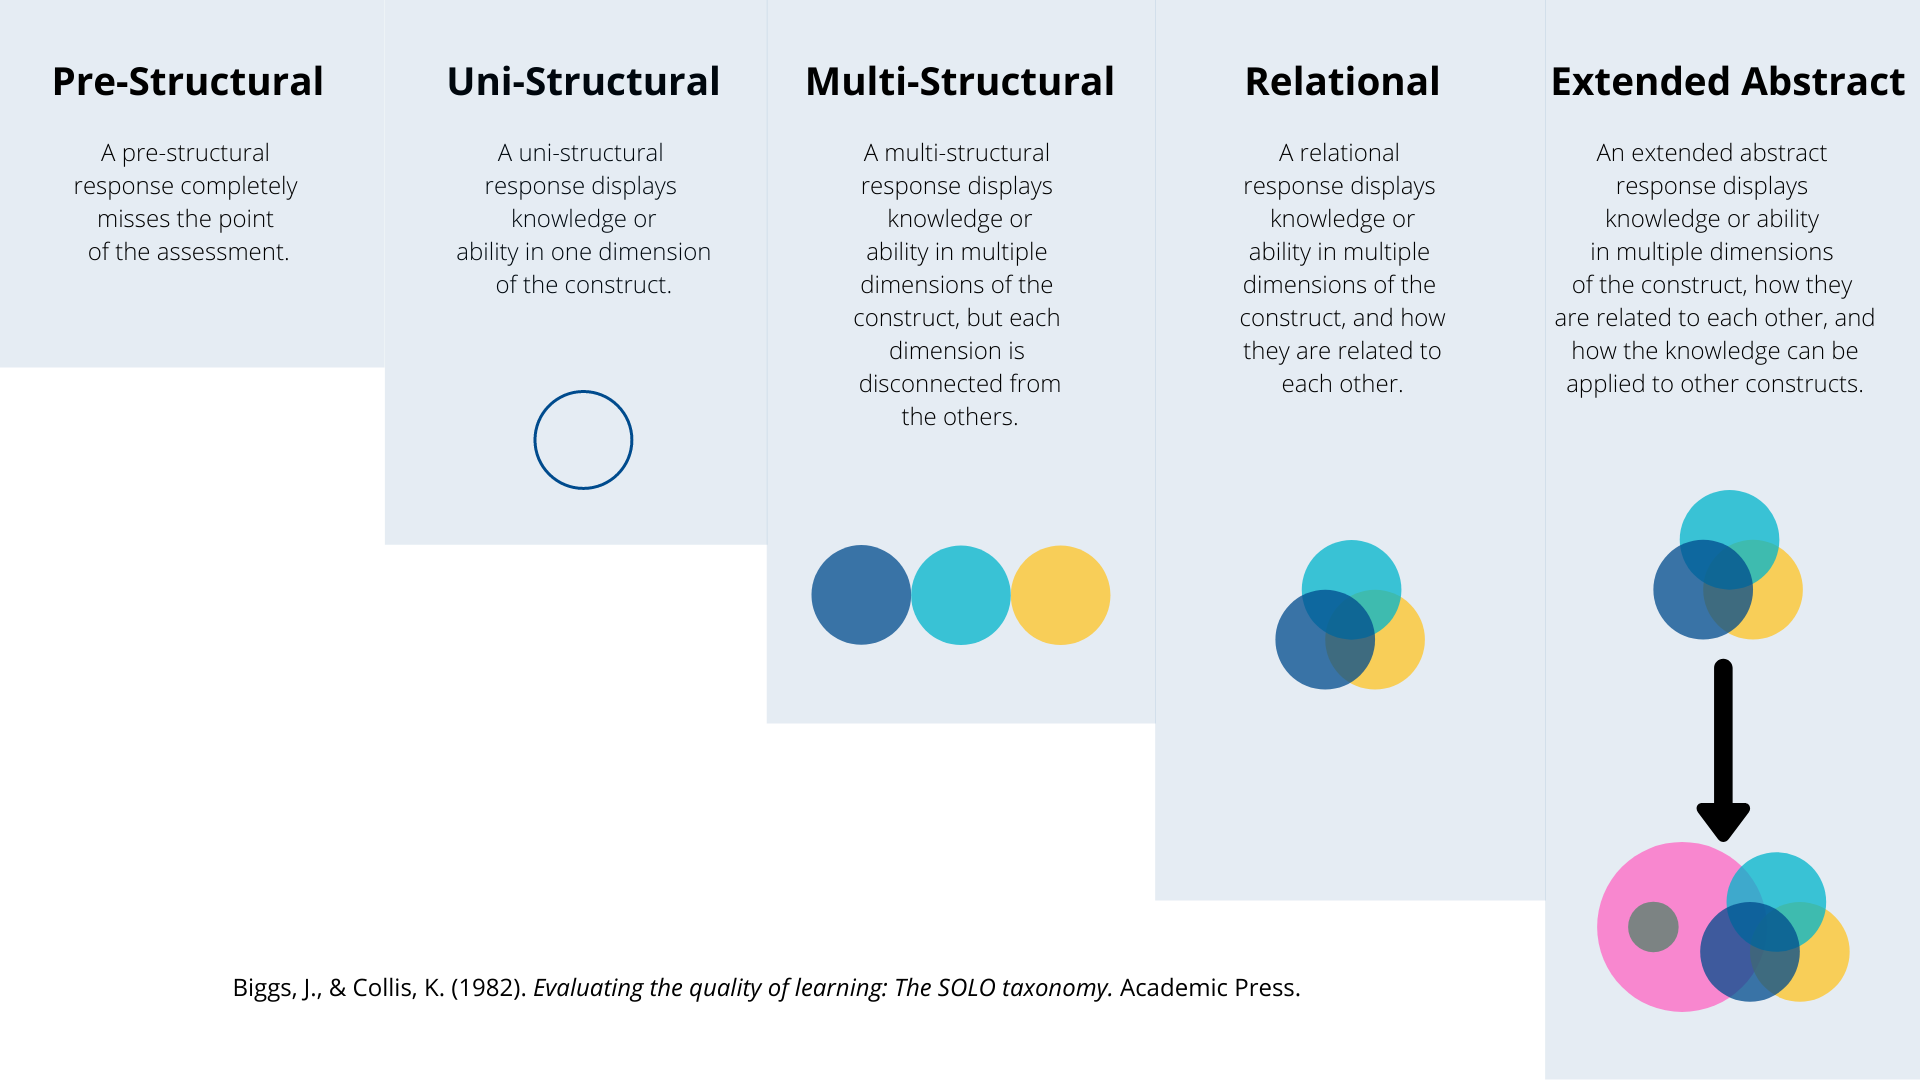
\includegraphics{assets/SOLO-taxonomy.png}
\caption{SOLO Taxonomy (adapted from Biggs \& Collis, 1982)}
\end{figure}

\hypertarget{pre-structural}{%
\subsubsection*{Pre-Structural}\label{pre-structural}}
\addcontentsline{toc}{subsubsection}{Pre-Structural}

A pre-structural response completely \textbf{\emph{misses the point}} of the assessment.

\hypertarget{uni-structural}{%
\subsubsection*{Uni-Structural}\label{uni-structural}}
\addcontentsline{toc}{subsubsection}{Uni-Structural}

A uni-strucutral response displays knowledge or ability in \textbf{\emph{one dimension of the construct}}.

\hypertarget{multi-structural}{%
\subsubsection*{Multi-Structural}\label{multi-structural}}
\addcontentsline{toc}{subsubsection}{Multi-Structural}

A multi-structural response displays knowledge or ability in \textbf{\emph{multiple dimensions of the construct}}, but each dimension is \textbf{\emph{disconnected}} from the others.

\hypertarget{relational}{%
\subsubsection*{Relational}\label{relational}}
\addcontentsline{toc}{subsubsection}{Relational}

A relational response displays knowledge or ability in \textbf{\emph{multiple dimensions of the construct, and how they are related to each other}}.

\hypertarget{extended-abstract}{%
\subsubsection*{Extended Abstract}\label{extended-abstract}}
\addcontentsline{toc}{subsubsection}{Extended Abstract}

An extended abstract response displays knowledge or ability in \textbf{\emph{multiple dimensions of the construct, how thy are related to each other, and how that construct can be applied to help us understand different constructs}}.

If you are providing responses at a \texttt{pre-\ or\ uni-structural} level in a graduate course, you are going to have a bad time. \texttt{Multi-structural} responses will lead to grades in the `C' range. At minimum, your responses should be \texttt{unambiguously\ relational} for a grade in the `B' range and \texttt{extended\ abstract} for a grade in the `A' range.

The \href{https://www.twu.ca/about/policies-guidelines/university-standard-grading-system}{TWU Grading Scale}, available on the syllabus for this course, describes A-, A, or A+ work as

\begin{quote}
\textbf{Outstanding, excellent work}; exceptional performance with strong evidence of original thinking, good organization, meticulous concern for documented evidence, and obvious capacity to analyze, synthesize, evaluate, discern, justify, and elaborate; frequent evidence of both verbal eloquence and perceptive insight in written expression; excellent problem-solving ability in scientific or mathematical contexts with virtually no computational errors; demonstrated masterful grasp of subject matter and its implications. Gives evidence of an extensive and detailed knowledge base. (Note: The A+ grade is reserved for very rare students of exceptional intellectual prowess and accomplishment, especially in lower level courses.)
\end{quote}

For a grade in the B-, B, or B+ range, here is what you need to do:

\begin{quote}
\textbf{Good, competent work}; laudable performance with evidence of some original thinking, careful organization; satisfactory critical and analytical capacity; reasonably error-free expository written expression, with clear, focused thesis and well-supported, documented, relevant arguments; good problem-solving ability, with few computational or conceptual errors in scientific subjects; reasonably good grasp of subject matter but an occasional lack of depth of discernment; evidence of reasonable familiarity with course subject matter, both concepts and key issues. Exhibits a serious, responsible engagement with the course content.
\end{quote}

We are happy to have a conversation with you if you feel your work has been unfairly assessed and you can provide a justifiable rationale based on the product of your work in relation to the requirements of the assignment and the standards outlined above and in the University Calendar.

\hypertarget{learning-in-community}{%
\chapter{Learning in Community}\label{learning-in-community}}

\begin{feedback}
{Things To Do This Week}

You will be directed when to complete the following tasks.

\begin{itemize}
\tightlist
\item
  Meet in Zoom \href{https://www.timeanddate.com/worldclock/fixedtime.html?msg=LDRS663+Meeting\&iso=20230913T10\&p1=256\&ah=1}{{Wednesday, September 13 - 10:00 AM PDT }(Click to check your local time)} ✅
\item
  Create a blog site \href{https://create.twu.ca}{on the TWU WordPress Network}. \href{https://ma-lead.github.io/ldrs663/wordpress}{Click here for instructions.}\\
\item
  \textbf{Read} \href{https://www-sciencedirect-com.twu.idm.oclc.org/science/article/pii/S1096751600000166}{Critical inquiry in a text-based environment: Computer conferencing in higher education}\\
\item
  \textbf{Read} \href{http://www.irrodl.org/index.php/irrodl/article/view/149/230}{Getting the mix right again: An updated and theoretical rationale for interaction}\\
\item
  \textbf{Read} \href{https://link-springer-com.ezproxy.student.twu.ca/article/10.1007/s12528-011-9049-4}{Interaction and the online distance classroom: Do instructional methods effect the quality of interaction?}\\
\item
  \textbf{Publish} your arguments for or against the \emph{Interaction Equivalency Theorem} on your blog..\\
\item
  Please complete these tasks by {Saturday, September 16} before your regular bedtime. The reason for this short week is that we want to start our weeks on Mondays. Don't worry too much if you don't get this one done right on time.
\end{itemize}
\end{feedback}

\hypertarget{overview}{%
\section*{Overview}\label{overview}}
\addcontentsline{toc}{section}{Overview}

Welcome to LDRS 663 - \emph{Coaching for Transformational Blended Learning}! In this second unit, we will begin by considering the nature of learning communities through the lens of a model called the \emph{Community of Inquiry (CoI)} (\href{https://www.sciencedirect.com/science/article/pii/S1096751600000166?}{Garrison et al., 2000}; \href{http://www.aupress.ca/index.php/books/120229}{Vaughan et al., 2013}). The CoI model proposes that there are three overlapping components, or presences, to any learning environment; cognitive presence (constructing meaning), social presence (projecting a sense of yourself), and teaching presence (designing and facilitating the learning experience). The CoI model is grounded in a long history of social constructivism which is the idea that learning is fundamentally a social process (\href{https://en.wikisource.org/wiki/My_Pedagogic_Creed}{Dewey, 1897}; \href{https://twu.idm.oclc.org/login?url=http://search.ebscohost.com/login.aspx?direct=true\&db=cat05965a\&AN=alc.191437\&site=eds-live}{Vygotsky, 1978}). We will also consider various modes of interaction in learning environments and how these two models have informed the model of teaching and learning in TWU FAR Centres.

\hypertarget{topics}{%
\subsection*{Topics}\label{topics}}
\addcontentsline{toc}{subsection}{Topics}

This unit is divided into 3 topics:

\begin{enumerate}
\def\labelenumi{\arabic{enumi}.}
\tightlist
\item
  Introduction to the Community of Inquiry Model\\
\item
  Modes of Interaction\\
\item
  Interaction Equivalency Theorem
\end{enumerate}

\hypertarget{learning-outcomes}{%
\subsection*{Learning Outcomes}\label{learning-outcomes}}
\addcontentsline{toc}{subsection}{Learning Outcomes}

When you have completed this unit you should be able to:

\begin{itemize}
\tightlist
\item
  Analyze the characteristics of the Community of Inquiry model.
\item
  Evaluate different modes of interaction.
\item
  Criticize the Interaction Equivalency Theorem.
\end{itemize}

\hypertarget{resources-1}{%
\subsection*{Resources}\label{resources-1}}
\addcontentsline{toc}{subsection}{Resources}

Here are the resources you will need to complete this unit:

\begin{itemize}
\tightlist
\item
  \href{https://www-sciencedirect-com.twu.idm.oclc.org/science/article/pii/S1096751600000166}{Critical inquiry in a text-based environment: Computer conferencing in higher education}\\
\item
  \href{http://www.irrodl.org/index.php/irrodl/article/view/149/230}{Getting the mix right again: An updated and theoretical rationale for interaction}\\
\item
  \href{https://rdcu.be/cKSGf}{Interaction and the online distance classroom: Do instructional methods effect the quality of interaction?}
\end{itemize}

\begin{blank}
{✨ ProTip}

Ok\ldots it would seem that the TWU library has lost access to the database that contains the Kanuka article above (`Interaction and the online distance classroom\ldots{}'). Here is how I go about tracking down articles In this case, I've completed all of the checked items and am waiting to hear back from Dr.~Kanuka):

✅ I see if I have access through another library. As a PhD candidate at UVic, I have access to their library, and it turns out that this article is in their collection, but that doesn't help you.\\
✅ I use a Firefox extension called `Unpaywall', which searches for open-access versions of the same article as researchers are often able to post pre-print versions of their article on their own site. In this case, unpaywall just links to the PDF that I have access to through UVic.\\
✅ I contact the \href{https://libguides.twu.ca/help}{TWU library} for assistance, as librarians are among the most helpful people on the planet. In this case, I was provided an open link, but that link looks fishy as it isn't apparently tied to Kanuka's site, but rather an aggregation site. Often, I also request an inter-library loan, in which the TWU library would contact another library (maybe UVic) and request a copy through them.\\
✅ Search \href{https://scholar.google.com}{Google Scholar} as that will often pick up on preprints on the author's website.\\
✅ Search \href{https://www.researchgate.net/}{ResearchGate} for preprints.\\
✅ Contact the author of the paper. They often have permission to share preprints (see above) and are usually happy to share their work, especially with grad students.\\
❌ Here is where we start getting into academic grey areas\ldots so don't do this. It is against publishers policy to use tools like the hashtag \#ICanHazPDF on Twitter, where you post the title of the article you are looking for under that hashtag and another researcher might respond by DM'ing you a copy. You shouldn't do this, because it cuts into the \textbf{\emph{absurd}} profits of massive multi-national corporations who benefit from the free work of researchers all over the world. This is nothing like walking down a hallway and knocking on your colleague's door to ask if they have a copy of a paper, because that is super illegal too and this is digital\ldots or something.

And this whole mess of strategies could be avoided if everyone published under an open license and the research that is created, usually with government funding, was freely available to those who need it.

{An update on this link\ldots{}}

✅ I received a response from the author, who generously provided a PDF copy of the article. This is very common.\\
✅ Also, I discovered at the bottom of the page when I viewed the article signed into a different library, that there was an option to get a sharing link, so I copied that link and updated the URL above. This seems to provide a read-only link for people who don't have access through a library or other institution.
\end{blank}

\begin{figure}
\centering
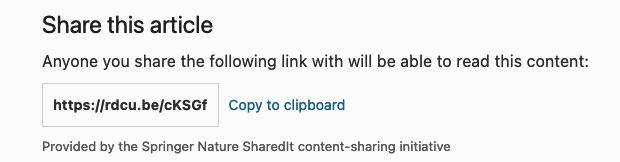
\includegraphics{assets/u2/share.png}
\caption{Share this article}
\end{figure}

\hypertarget{optional-resource}{%
\subsubsection*{Optional Resource}\label{optional-resource}}
\addcontentsline{toc}{subsubsection}{Optional Resource}

\begin{itemize}
\tightlist
\item
  Vaughan, N., Cleveland-Innes, M., \& Garrison, D. (2013). \emph{Teaching in blended learning environments: Creating and sustaining communities of inquiry.} Athabasca: AU Press. - This book is available for free at \href{http://www.aupress.ca/index.php/books/120229}{AUPress}.
\end{itemize}

\hypertarget{introduction-to-the-community-of-inquiry-model}{%
\section{Introduction to the Community of Inquiry Model}\label{introduction-to-the-community-of-inquiry-model}}

Before you dive into the content of this unit in LDRS 663, take a moment to recall some particularly memorable learning experiences that you have had. They don't have to be particularly profound in terms of \emph{what} you learned, but profound because of the fact that you still remember \emph{that} you learned something and \emph{how} you learned it. Pick one or two of those experiences and be prepared share them in our class meeting. Make sure to tell us about the context of your experience. Who was there? What did you do to learn? Why do you remember it?

\hypertarget{social-constructivism}{%
\subsection*{Social Constructivism}\label{social-constructivism}}
\addcontentsline{toc}{subsection}{Social Constructivism}

There is a very good chance that your recollection of a memorable learning experience as part of the previous learning activity included a description of some sort of social interaction. This isn't always the case, but the idea that learning is a social process has a long history in education. Many theorists credit John Dewey for bringing this idea to the forefront of educators' minds. In his 1897 treatise \emph{My Pedagogic Creed} he writes:

\begin{quote}
I believe that the school is primarily a social institution. Education being a social process, the school is simply that form of community life in which all those agencies are concentrated that will be most effective in bringing the child to share in the inherited resources of the race, and to use his own powers for social ends. (p.~7)
\end{quote}

The idea didn't originate with Dewey, though, as we know that in first-century Palestine there was a certain itinerant teacher whose lessons were profoundly impactful on a small group of young men and women who were called to live and learn in a deeply personal and social community.

Following Dewey, many others, such as Jean Piaget, Jerome Bruner, and Lev Vygotsky (see \href{https://twu.idm.oclc.org/login?url=http://search.ebscohost.com/login.aspx?direct=true\&db=cat05965a\&AN=alc.1254633\&site=eds-live}{Driscoll, 2005)} have written about what has now become known as the educational theory of \emph{social constructivism}, or, more concisely, constructivism. Driscoll (2005) describes constructivism as a theory that
\textgreater{} rests on the assumption that knowledge is constructed by learners as they attempt to make sense of their experiences. Learners, therefore are not empty vessels waiting to be filled, but rather active organisms seeking meaning. (p.387)

This process of seeking meaning is an iterative process whereby the learner experiences some sort of cognitive dissonance, or a disconnect between what they previously knew and some new piece of evidence or experience that disconfirms that knowledge. The learner then seeks to resolve that dissonance by either incorporating the new experience into an older schema, or by disregarding one or the other. Most often, the resulting knowledge is constructed from portions of both the new and old idea.

\hypertarget{community-of-inquiry}{%
\subsection*{Community of Inquiry}\label{community-of-inquiry}}
\addcontentsline{toc}{subsection}{Community of Inquiry}

This brings us to the idea of a `Community of Inquiry' (CoI), which was first described by Garrison, Anderson, and Archer in their 2000 article ``Critical Inquiry in a text-based environment''. Garrison, et al.~theorize that there are three critical components, or ``presences'' that compose an interactive, online learning environment: Cognitive presence, social presence, and teaching presence. The intersection of these three presences is the heart of an educational experience.

\begin{figure}
\centering
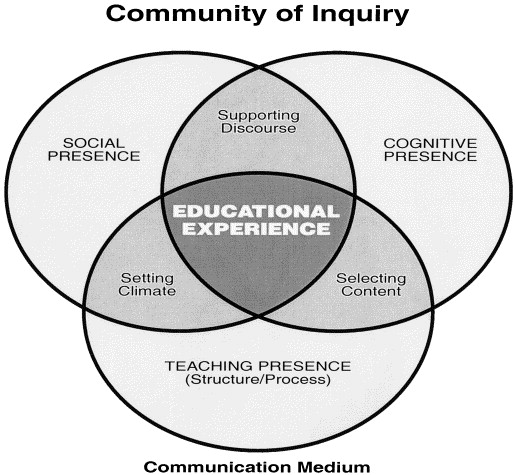
\includegraphics{assets/u2/CoI-Model.jpg}
\caption{Community of Inquiry Model (Garrison, et al., (2000)}
\end{figure}

\hypertarget{cognitive-presence}{%
\subsubsection*{Cognitive Presence}\label{cognitive-presence}}
\addcontentsline{toc}{subsubsection}{Cognitive Presence}

Cognitive presence, possibly the most foundational element, is the
\textgreater{} extent to which the participants in any particular configuration of a community of inquiry are able to construct meaning through sustained communication (p.~89).

Recall that this cognitive process is at the heart of constructivist learning environments. It seems obvious (be careful when people say that) that this construction of meaning through communication is the entire point of higher education. Your task as a student is to change your own mind, and that is a very tall order as our beliefs about many things are remarkably resilient. The way we engage in this task will have a significant bearing on the outcomes of the task.

If we approach communication with too much confidence in our own views, we can shut out competing ideas to our own detriment, so it is important to bring a cautious intelligence, or, as I once heard a student describe it, epistemic humility. We all know that we are wrong about some things. The trouble is we don't know what we are wrong about and how we have misunderstood.

Cognitive presence in a text-based environment (like an online course) carries with it some affordances, but also some disadvantages. It is a relatively common experience for people to type something in a text message or an email, only to have their intentions grossly misunderstood because there are fewer para-linguistic cues in text compared to verbal face-to-face communication. Recent developments in incorporating emojis have started to change this, but emojis are generally considered to be too informal for `serious scholarly work' or written professional communication. So, the relatively lean environment of text can lead to significant misunderstandings.

On the other hand, for learners like me who tend toward introversion, the asynchronous nature of text-based learning environments is a huge advantage. I couldn't count the number of times that I have wanted to contribute to an in-class discussion, but needed too much time to formulate a coherent response, and before I knew it, the conversation had moved on. My point was no longer relevant, having been resolved by those in the class who were more extroverted and ready with an answer. A text-based environment, however, gives me \emph{time to think, write, revise, and then post} my response.

\hypertarget{social-presence}{%
\subsubsection*{Social Presence}\label{social-presence}}
\addcontentsline{toc}{subsubsection}{Social Presence}

Garrison, et.al. describe social presence as
\textgreater the ability of participants in the Community of Inquiry to project their personal characteristics into the community, thereby presenting themselves to the other participants as ``real people.'' (p.~89)

In any community, and especially the TWU community, the ability to \emph{belong} and to be accepted as a whole and integrated person is critical to people feeling like they \emph{actually do belong}. It is for this reason that many experienced online educators encourage a more colloquial style of writing in online forums or blogs. Strict adherence to APA or other style guides virtually eliminates self-referential language such as personal pronouns. It is hard to project your personal characteristics as a real person when you can only refer to yourself in the third person.

By allowing a more personal style and the projection of self into the community, it is thought that students will build a sense of trust in the community and feel more empowered to participate in the difficult work of changing their minds. Social presence supports cognitive presence by allowing the learning environment to be safe and welcoming.

\hypertarget{teaching-presence}{%
\subsubsection*{Teaching Presence}\label{teaching-presence}}
\addcontentsline{toc}{subsubsection}{Teaching Presence}

This final element of the CoI model is the design and facilitation of the learning experience
\textgreater to support and enhance social and cognitive presence for the purpose of realizing educational outcomes. (p.~90).

Teaching presence can be a shared function between members of the community. Garrison, et al.~point out that the design of the experience is typically performed by the teacher, and the facilitation is more often shared. In a connected course like this one, there is a greater emphasis on shared facilitation in a community of learners compared to what might be experienced in a f2f (face to face) course. It is in this shared discourse in a safe environment that allows learners to engage in the difficult cognitive work of learning.

\hypertarget{learning-activity}{%
\subsection*{Learning Activity}\label{learning-activity}}
\addcontentsline{toc}{subsection}{Learning Activity}

\begin{reflect}
{Read, Annotate, and Reflect}

\textbf{Read} \href{https://www-sciencedirect-com.twu.idm.oclc.org/science/article/pii/S1096751600000166}{Critical inquiry in a text-based environment: Computer conferencing in higher education} (access through the TWU library).

If you haven't done so previously, sign up for and activate hypothes.is and while you are reading the article, leave some annotations that connect what you are reading to your own experience.

Use the tag `ldrs663' in any annotations you create so that we can all find each other.

\href{http://create.twu.ca/help/other-web-tools/hypothesis}{Click here for assistance getting set up with hypothes.is.}

As you read, consider a time where you experienced a learning environment where the three presences described in the CoI were apparent. Consider the following questions and optionally, write your responses in a new post on your blog.
- Were all three presences demonstrated?
- Which of the three were most obvious? Least?
- Which presence is most important for you?

Note that this is an ungraded activity, but is designed to help prepare you for the assessments in this course. Throughout the course you are encouraged to take notes in a journal of some sort. Refer to these notes as you complete your assessments.
\end{reflect}

\hypertarget{modes-of-interaction}{%
\section{Modes of Interaction}\label{modes-of-interaction}}

For this next topic we will look at what we mean by `interaction', a word which is thrown around a lot in educational technology, but\ldots{}

\href{https://youtu.be/G2y8Sx4B2Sk}{Watch}

Before we get into the the topic of interaction, please take a few minutes to answer the following questions about scenarios that may or may not be considered `interaction'.
(Note that you can check your answer right away, and then click the arrow for the next example.)

What do you think? Do you agree with the `correct' and `incorrect' responses on the quiz?

\hypertarget{interaction}{%
\subsection*{Interaction}\label{interaction}}
\addcontentsline{toc}{subsection}{Interaction}

Anderson (2003) argues that, despite the lack of clarity around definitions of interaction, there seems to be a general understanding that interaction of some sort is a requirement for learning. He settles on the definition from Wagner (1994, p.8)

\begin{quote}
reciprocal events that require at least two objects and two actions. Interactions occur when these objects and events mutually influence one another.
\end{quote}

He provides a model of interaction in learning environments that includes three main agents in the process: students, teachers, and content (Figure 1).

\begin{figure}
\centering
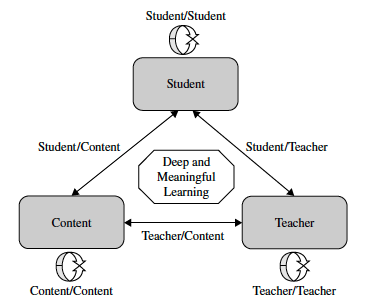
\includegraphics{assets/u2/Modes-Interaction-Anderson.png}
\caption{Figure 1. Anderson's Modes of Interaction (2003)}
\end{figure}

At each point of the triangle are the agents in an educative process. The arrows between them indicate the two-way communication described by Wagner, and the recursive arrows above or below the agents are secondary forms of interaction.

\hypertarget{other-models-of-interaction}{%
\subsection*{Other Models of Interaction}\label{other-models-of-interaction}}
\addcontentsline{toc}{subsection}{Other Models of Interaction}

Kanuka (2011) describes a modified model of interaction which presumes that all educational interactions occur in the context of some sort of content (Figure 2.).

\begin{figure}
\centering
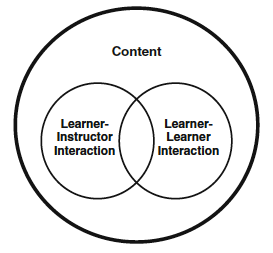
\includegraphics{assets/u2/Kanuka-Modes-of-Interaction.png}
\caption{Figure 2. Kanuka's Model of Interaction (2011)}
\end{figure}

In Anderson's model, content is an agent in the process, but in Kanuka's model, content of some sort is assumed to be the foundation of learning environments and that interactions between and among learners and instructors happens in the context of making sense of the content. The content itself does not have agency.

A combination of these two models was described by Madland (2014). Madland's model, shown in figure 3, is a return to Anderson's three-sided model except with the addition of peer interactions, and all interactions between agents occuring in the context of the content that is to be learned. Also added are the three sides of the model representing structured learning activities designed specifically to enhance the educative effects of the interactions.

\begin{figure}
\centering
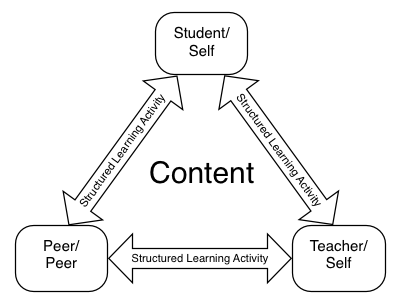
\includegraphics{assets/u2/Modes-of-Interaction-Madland.png}
\caption{Figure 3. Madland's Model of Interaction (2014)}
\end{figure}

It is not enough to simply expect interactions between learners and instructors to be goal-oriented towards learning outcomes. Educators must design specific activities (teaching presence) to create the conditions (social presence) for learning to occur (cognitive presence). An example of this can be seen in the seemingly ubiquitous `Group Project' assigned in so many undergraduate courses. Sometimes, groups are allowed to form themselves, other times, the instructor assigns groups, or there is some sort of random process to create groups. However they are formed, groups too often fall into a pattern of behaviour where one or two of the students do most of the work and the remaining group members engage in social loafing and benefit from their peers' work.

An alternative practice is to engage groups in a specific structured process of cooperation where everybody must do their work, or else the entire group suffers. An example is to have students work in peer review partners where students submit their assignments to their peer review partner who then provides feedback based on specific questions and categories of comments. When the original students receives their partner's feedback, they may choose how to integrate the suggestions into the final assignment that they submit to their instructor. Each student is then graded on the quality of their finished assignment, the quality of the feedback that they provided, and on the rationale for how they incorporated the peer review into their own work.

There are myriad structures that can be used to ensure that interactions are inclined towards producing student learning, and we will introduce you to some of those in unit 5.

\hypertarget{learning-activity-1}{%
\subsection*{Learning Activity}\label{learning-activity-1}}
\addcontentsline{toc}{subsection}{Learning Activity}

\begin{reflect}
Read the following article by Terry Anderson
- \href{http://www.irrodl.org/index.php/irrodl/article/view/149/230}{Getting the mix right again: An updated and theoretical rationale for interaction}

As you read, consider what interactions you have experiences in online or f2f courses.
\end{reflect}

\hypertarget{interaction-equivalency-theorem}{%
\section{Interaction Equivalency Theorem}\label{interaction-equivalency-theorem}}

For our last topic of this unit, we'll explore Anderson's (2003) \emph{Interaction Equivalency Theorem}, stated as

\begin{quote}
Deep and meaningful formal learning is supported as long as one of the three forms of interaction (student--teacher; student-student; student-content) is at a high level. The other two may be offered at minimal levels, or even eliminated, without degrading the educational experience.
High levels of more than one of these three modes will likely provide a more satisfying educational experience, though these experiences may not be as cost or time effective as less interactive learning sequences. (p.~4)
\end{quote}

At TWU, there has always been a significant emphasis placed on student-teacher interactions. This can be seen in small class sizes and opportunities for students to be involved in faculty-led research projects and travel studies. Distance education, however, has long suffered from a distinct lack of student-teacher and student-student interactions. For many years, distance education was delivered either through the post or through one-way media such as radio or TV, virtually eliminating interactions. This led to a pervasive view that distance education courses and programs were second-rate at best.

However, now that modern communication infrastructure has developed to the point that media-rich, synchronous, two-way communication is almost free, opportunities for distance learning environments to include high levels of student-student and student-teacher interaction are much more feasible.

One problem remains, though, and that is that student-teacher interaction is a scarce commodity. It is costly to hire enough faculty to enable one-on-one or small-group interaction between students and faculty. The distance educator's response to this challenge is to front-load the faculty input (high-level disciplinary expertise or cognitive presence) into the course materials and to de-couple `interaction' from both time and place.

In an asynchronous, text-based environment, students and teachers do not need to be present in the same place at the same time in order to enjoy rich interactions.

\hypertarget{unit-1-assessment}{%
\section*{Unit 1 Assessment}\label{unit-1-assessment}}
\addcontentsline{toc}{section}{Unit 1 Assessment}

\begin{wp}
{WordPress Post}

Please complete the assignment under `Post 1' below. This will be your first of \st{five} four draft posts during the course.

\href{https://ma-lead.github.io/ldrs663/assessments.html\#post-1}{Blog Post 1}
\end{wp}

\hypertarget{references}{%
\section*{References}\label{references}}
\addcontentsline{toc}{section}{References}

Anderson, T. (2003). Getting the mix right again: An updated and theoretical rationale for interaction. \emph{International Review of Research in Open and Distance Learning,} 4(2), 1--14.

Dewey, J. (1897). \emph{My pedagogic creed.} In M. S. Dworkin (Ed.), \emph{Dewey on education.} NewYork, NY: Teachers College Press.

Driscoll, M. P. (2005). \emph{Psychology of learning for instruction} (3rd ed.). Boston: Pearson Education.

Garrison, D. R., Anderson, T., \& Archer, W. (2000). Critical inquiry in a text-based environment: Computer conferencing in higher education. \emph{The Internet and Higher Education, 2}, 87--105. \url{https://doi.org/10.1016/S1096-7516(00)00016-6}

Kanuka, H. (2011). Interaction and the online distance classroom: Do instructional methods effect the quality of interaction? \emph{Journal of Computing in Higher Education,} 23(2), 143--156. \url{https://doi.org/10.1007/s12528-011-9049-4}

Madland, C. (2014). \emph{Structured student interactions in online distance learning: Exploring the study buddy activity} (Master's thesis). Athabasca University. Retrieved from \url{http://hdl.handle.net/10791/47}

\hypertarget{learning-facilitation}{%
\chapter{Learning Facilitation}\label{learning-facilitation}}

\begin{feedback}
{Things To Do This Week - actually, 2 weeks!}

\begin{itemize}
\tightlist
\item
  Meet in Zoom {Wednesday, September 20, 10:30 am PDT} \href{https://www.timeanddate.com/worldclock/fixedtime.html?msg=LDRS663+Meeting\&iso=20230920T1030\&p1=256\&ah=1}{Check your local time here}
\item
  Meet in Zoom {Wednesday, September 27, 10:30 am PDT} \href{https://www.timeanddate.com/worldclock/fixedtime.html?msg=LDRS663+Meeting\&iso=20230927T1030\&p1=256\&ah=1}{Check your local time here}
\item
  If you haven't already, sign up for a Learning Pod. Link is in Moodle.
\item
  \textbf{Read} \href{https://infed.org/mobi/facilitating-learning-and-change-in-groups-and-group-sessions/}{\textbf{Facilitating Learning and Change in Groups}}\\
\item
  \textbf{Read} \href{https://infed.org/mobi/what-is-a-group/}{\textbf{What is a Group?}}\\
\item
  \textbf{Read} \href{https://www.researchgate.net/publication/228957278_From_Comfort_Zone_to_Performance_Management}{\textbf{Comfort Zone to Performance Management}}

  \begin{itemize}
  \tightlist
  \item
    \href{assets/Performance_Management.pdf}{PDF Download}
  \end{itemize}
\item
  \textbf{Read} \href{https://www.iaf-world.org/site/professional/core-competencies}{\textbf{Core Competencies}}

  \begin{itemize}
  \tightlist
  \item
    \href{assets/core-comp.pdf}{PDF Download}
  \end{itemize}
\item
  \textbf{Watch} \href{https://player.vimeo.com/video/364868276}{Liberating Structures}\\
\item
  \textbf{Visit} \href{http://www.liberatingstructures.com/9-what-so-what-now-what-w/}{\textbf{What, So What, Now What? W³}}\\
\item
  \textbf{Publish} \href{https://ma-lead.github.io/ldrs663/assessments.html\#post-2}{Post \#2}
  ✅ Please complete these items by {Saturday, September 30 - by sundown}
\end{itemize}
\end{feedback}

\begin{blank}
\hypertarget{note}{%
\subsubsection*{✨ NOTE}\label{note}}
\addcontentsline{toc}{subsubsection}{✨ NOTE}

Your \href{https://far.twu.ca/ldrs/663-202109/assignments}{\textbf{Small Group Facilitation Session}} is due {\textbf{\emph{Saturday, September 30}}}. Please begin scheduling your facilitation sessions with your groups this week so you have enough time to complete the sessions and your reflections.
\end{blank}

\hypertarget{overview-1}{%
\subsection*{Overview}\label{overview-1}}
\addcontentsline{toc}{subsection}{Overview}

Facilitation in education refers to the process of helping learners to explore, learn and change. A facilitator is expert on process and group interactions. In education, facilitation is rooted in understanding the nature of the social learning process and how to guide its direction and quality. As a social species, we learn a great deal from each other in both formal and informal contexts. Our earliest learning experiences are profoundly social and intimate interactions between mother and child, and the social aspect of learning never ceases to be important. During this unit, we will examine a short history of social theories of learning from John Dewey and Lev Vygotsky, then, we will experiment with the theory and practices of facilitating learning in group settings.

\hypertarget{topics-1}{%
\subsection*{Topics}\label{topics-1}}
\addcontentsline{toc}{subsection}{Topics}

This unit is divided into the following topics:

\begin{enumerate}
\def\labelenumi{\arabic{enumi}.}
\tightlist
\item
  Social Theories of Learning
\item
  Cooperative Learning
\item
  Facilitating Transformational Learning in Group Settings
\item
  Navigating Group Dynamics
\item
  Core Facilitation Competencies
\item
  Strategies for Learning Facilitation
\end{enumerate}

\hypertarget{learning-outcomes-1}{%
\subsection*{Learning Outcomes}\label{learning-outcomes-1}}
\addcontentsline{toc}{subsection}{Learning Outcomes}

When you have completed this unit, you should be able to:

\begin{itemize}
\tightlist
\item
  Explain how to design learning environments to maximize learning
\item
  Plan appropriate group learning processes to support transformative learning.
\item
  Demonstrate how to facilitate a course of study.
\item
  Design cooperative activities to maximize student-student and student-content interactions
\item
  Apply knowledge of the Community of Inquiry model and liberating structures to the facilitation of cooperative learning activities
\item
  Identify and explain core competencies for facilitating learning.
\end{itemize}

\hypertarget{resources-2}{%
\subsection*{Resources}\label{resources-2}}
\addcontentsline{toc}{subsection}{Resources}

Online resources will be provided in the unit.

\hypertarget{social-theories-of-learning}{%
\section{Social Theories of Learning}\label{social-theories-of-learning}}

The idea that learning is a social process can be traced way back in time, but formal descriptions of social constructivism, as it has been called, are often traced to John Dewey, Jean Piaget, and Lev Vygotsky. Albert Bandura also contributed via social learning theory. \emph{What is social constructivism?}

Vygotsky (1978) argues that ``every function in the child's cultural development appears twice: first, on the social level, and later on the individual level; first \emph{between} people (\emph{interpsychologically}), and then inside the child (\emph{intrapsychologically}) (p.~57). That is, humans learn first through social observations and interactions, which they later internalize as their own thinking. The significance of Vygotsky's insight is that, ``instead of focusing on the study of psychological entities such as skills, concepts, information-processing units, reflexes, or mental functions, it assumes that we must begin with a unit of \emph{activity''} (Wertsch, 1985). This idea of \emph{activity,} or to be more precise the active participation of the learner, is central to our emerging understanding of learning as a process of socially constructing knowledge.

Central to this progress is language, which we first learn in the context of social interactions, then, we adopt as self-talk for self-direction and self-regulation, and ultimately internalized as our own inner speech (Vygotsky \& Kozulin, 1986, p.~228). Similarly, Bandura (1977) argues social role modeling is central to how most behaviors are learned, ``from observing others one forms an idea of how new behaviors are performed, and on later occasions this coded information serves as a guide for action''.

In sum, we may conclude that knowledge is \emph{constructed} first socially, then, personally, by learners as they encounter new information, compare it to old models that they may have, and develop new understandings of how the world works. It is not the case that new knowledge is simply copied intact from one mind to another, rather new information is integrated into old understandings, bringing about a hybrid of the two. This is essentially what we understand as a \emph{constructivist} model of learning.

\hypertarget{zone-of-proximal-development}{%
\subsection*{Zone of Proximal Development}\label{zone-of-proximal-development}}
\addcontentsline{toc}{subsection}{Zone of Proximal Development}

Social constructivism builds on the constructivist model, adding the idea that this process of integrating new understandings with old understandings is best understood as a \emph{social} process. Vygotsky (1978) introduced the idea that people with a greater capacity to understand the world and cope with its challenges act as supportive structures, which enable others to \emph{construct} and \emph{internalize} the knowledge these people have. This new construction occurs within what Vygotsky refers to as an individual's \textbf{\emph{zone of proximal development,}} which he differentiated from their \textbf{\emph{zone of actual development.}} The ZPD is the `sweet spot' in education where a student is optimally challenged to learn. If the task is too easy for the student, and they have already mastered it, then learning activities will not result in learning. Conversely, if a task is so difficult that the student cannot complete it, even with assistance, learning activities will not result in learning. In the middle are tasks that a student is able to complete, but only with the assistance of a more capable peer or expert. This is the Zone of Proximal Development:

\begin{figure}
\centering

\includegraphics{assets/u3/ZPD_Image.png}
\caption{Zone of Proximal Development}
\end{figure}

\hypertarget{scaffolding}{%
\subsection*{Scaffolding}\label{scaffolding}}
\addcontentsline{toc}{subsection}{Scaffolding}

A metaphor that has been used to describe one such supportive mechanism is \emph{scaffolding.} A scaffold is a way for educators to support the construction of new knowledge, beginning from a person's existing repertoire of knowledge and then preceding into new heights of understanding. The scaffold is the environment an educator creates, the support of learning facilitation, and the processes and language that are lent to the learner in the context of approaching an adaptive task and developing new abilities to meet it (Wilhelm, Baker, \& Dube, 2001). Furthermore, scaffolding implies not only a person's specific relation to the modeled behavior of others; it implies a person's relation to social communities, and ``it implies becoming a full participant, a member, a kind of person'' (Lave \& Wenger, 1996).

The task of facilitating learning with the ZPD in mind assumes that you, as the facilitator, know what knowledge and skills your students are starting with. It is likely that the competencies your students display fall along a bell curve. While most students will be learning within a similar ZPD, there will be outliers at both ends of the curve. One strategy can be to pair students whose skills and knowledge are below the curve with those above the curve. In doing this, students who are above the curve, who may not be challenged with the content or skill, have to engage in greater levels of cognitive complexity in order to concisely explain to their peer and help them to meet the objective. For example, Madland and Richards (2016) describes a cooperative peer review activity, where the authors asked a group of learners how they thought cooperative learning activities supported learning. In this study, the learners' responses indicated that the two most important factors were \emph{social cohesion} and \emph{developmentally appropriate challenges,} indicating that learners recognized the importance of the ZPD in learning.

\begin{reflect}
\hypertarget{learning-activity-2}{%
\subsubsection{Learning Activity}\label{learning-activity-2}}

\textbf{\emph{Questions to Consider}}\\
After reading the topic above, consider the following question:\\
- How does the idea of the zone of proximal development help you support learning?
\end{reflect}

\hypertarget{cooperative-learning}{%
\section{Cooperative Learning}\label{cooperative-learning}}

Cooperative learning is a set of learning facilitation strategies that are focused on encouraging educative social interactions between learners. It is important to not conflate \emph{cooperative learning} with \emph{group projects} as you might remember them from your previous experiences as a university student. Group projects are often assigned because faculty seem to have a sense that \emph{working together} is a good thing for students, along with a vague sense that modern jobs all require teamwork. Too often, they amount to repurposing an individual assignment (such as, a research paper) into the same task, but with multiple people handing in one item instead of three to four. When these tasks are not well structured, the process becomes problematic.

\begin{figure}
\centering
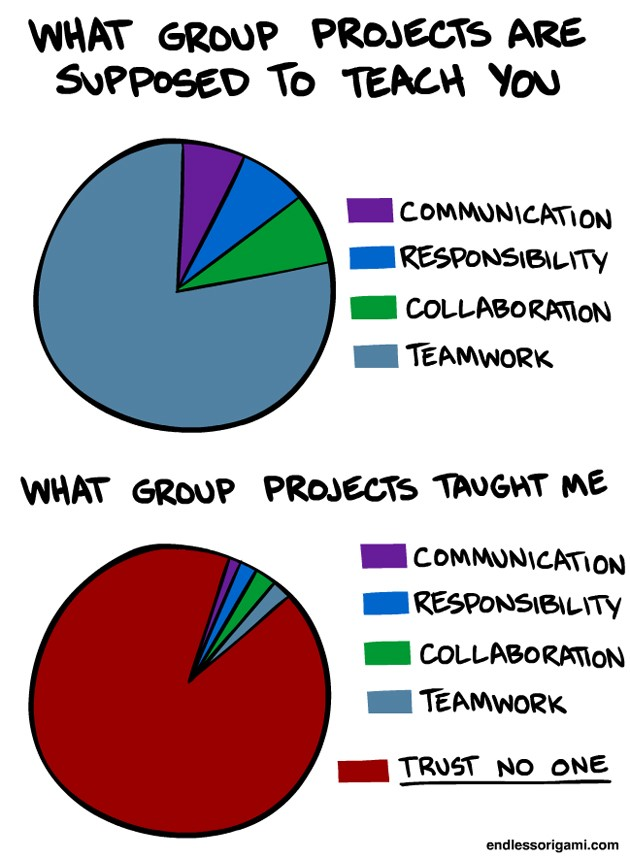
\includegraphics{assets/u3/U5_T2_Image.jpg}
\caption{Group Projects}
\end{figure}

We have all likely experienced less-than-ideal group projects where one or two people do most of the work, one member is seemingly absent altogether, and another's work is of poor quality. This is not the kind of learning activity that inspires highly engaged learners.

Contrary to this dysfunctional group learning model, cooperative learning is structured in a way that maximizes effort from all students and, ideally, leads to all group members attaining high-level learning outcomes. In order to ensure this, there are five characteristics of learning groups that must be present for cooperative learning to occur: \emph{``positive interdependence, individual accountability, promotive interactions, appropriate use of social skills, and group processing''} (Johnson \& Johnson, 2009, p.~366).

\hypertarget{more-about-cooperative-learning}{%
\subsubsection*{More about cooperative learning\ldots{}}\label{more-about-cooperative-learning}}
\addcontentsline{toc}{subsubsection}{More about cooperative learning\ldots{}}

\hypertarget{positive-interdependence}{%
\paragraph*{Positive Interdependence}\label{positive-interdependence}}
\addcontentsline{toc}{paragraph}{Positive Interdependence}

Positive interdependence, according to Johnson and Johnson is the idea that individuals in a learning environment are dependent upon each other for success. In other words, I cannot succeed unless you succeed and you cannot succeed unless I succeed. So, collectively, we are interdependent. Positive interdependence is the key that distinguishes cooperative learning from competitive learning, where students are graded on a curve and only the top 2-3\% of students can earn `A' grades.

\hypertarget{individual-and-group-accountability}{%
\paragraph*{Individual and Group Accountability}\label{individual-and-group-accountability}}
\addcontentsline{toc}{paragraph}{Individual and Group Accountability}

In cooperative learning environments, each individual in the group is held accountable for their contributions to the final product, and feedback is provided to both the individual and the group. This helps to ensure that students who need more assistance are identified and can be supported as needed, and it also prevents the `social loafing' that is common in typical `group projects.'

\hypertarget{promotive-interaction}{%
\paragraph*{Promotive Interaction}\label{promotive-interaction}}
\addcontentsline{toc}{paragraph}{Promotive Interaction}

Promotive interaction is the logistics of working and learning together as a cooperative group. The essence is that group members each need to work to promote the learning of each other member of the group. Since each person will be held accountable for their work and the entire group will only succeed if each member succeeds, there is a natural social pressure on more experienced members of the group to assist those with less experience or knowledge.

\hypertarget{interpersonal-skills}{%
\paragraph*{Interpersonal Skills}\label{interpersonal-skills}}
\addcontentsline{toc}{paragraph}{Interpersonal Skills}

Not only do members of the group need to learn the content of the lesson or project, but they must also learn the process of working well as a cooperative group. Sometimes, these processes need to be taught directly, other times (like in graduate studies) it is reasonable to presume that group members will already possess and be willing to utilize effective social skills.

\hypertarget{group-processing}{%
\paragraph*{Group Processing}\label{group-processing}}
\addcontentsline{toc}{paragraph}{Group Processing}

Finally, the group must be able to monitor their process with the goal of improving their work process and product. This metacognitive task is crucial to the long-term improvement and progress towards learning goals.

\begin{figure}
\centering
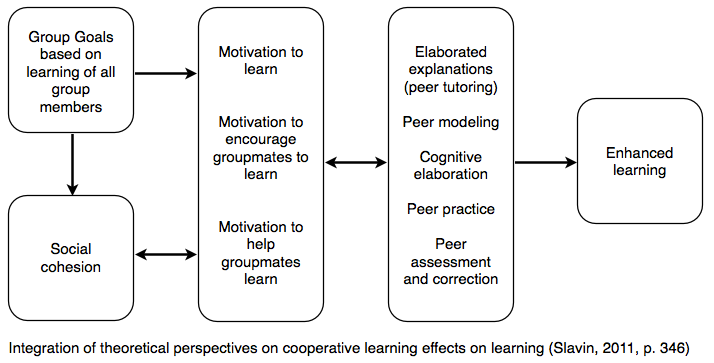
\includegraphics{assets/u3/Image3.png}
\caption{Cooperative Learning (Slavin, 2011)}
\end{figure}

\begin{reflect}
\hypertarget{learning-activity-3}{%
\subsubsection*{Learning Activity}\label{learning-activity-3}}
\addcontentsline{toc}{subsubsection}{Learning Activity}

\textbf{\emph{Questions to Consider}}\\
After reading through the content in Topic 2, please consider the following questions:\\
- How can coaching concepts be applied to helping learners learn?\\
- What key characteristics define effective coaching for learning?\\
- How can educators coach learners through the transition of making a change?
\end{reflect}

\hypertarget{facilitating-transformational-learning-in-group-environments}{%
\section{Facilitating Transformational Learning in Group Environments}\label{facilitating-transformational-learning-in-group-environments}}

In Unit One, we examined the CoI model and identified how teaching presence helps to support both the cognitive and social presences within the educational experience of a course of study. An important idea we emphasized was that teaching presence can be a shared function between members of the learning community and that facilitation of the learning process is often shared (Garrison, et al., 2010). Now, we are interested in examining what a division of the teaching presence might look like if we professionalize the function of learning facilitation within a distributed model of teaching presence.

Our prototype for exploring this model is TWU's own Facilitated Academic Resource (FAR) centre. The facilitation of courses in the TWU FAR Centre model is unique, as you know. From the perspective of a traditional, campus-based faculty member in Langley, a FAR Centre course is an \emph{online} course. The faculty member has worked in the role subject matter expert with an instructional designer to \emph{structure} a course which integrates everything required to create an online community of inquiry with allowances for all three presences: social, cognitive, and teaching. The courses are deployed through online technology and materials are accessed digitally in remote locations. Furthermore, students submit their work to the faculty member who then assesses their work and provides both formative and summative feedback as appropriate.

From the perspective of the remote student, however, the course is much more like a typical F2F course where they are meeting with a group of their fellow students in regularly scheduled learning labs in a central location and are guided through the learning materials by an experienced facilitator.

The rationale for this model is that international students often experience difficulties completing online courses from Western universities, so TWU is providing a F2F Academic Facilitator to support remote students in their individual and group studies through the courses. You, as the Academic Facilitation Specialist, are a critical component of this model. Your skills in coaching facilitating student learning through courses where you may not be a subject matter expert are going to be extremely important.

As such, you will need to start thinking about \emph{how} to facilitate your students' experience of a course of study's learning activities without the immediate F2F presence of a faculty member. In the activity below, you will read about the concept and practices of facilitating transformation learning.

\hypertarget{facilitating-group-learning-sessions}{%
\subsection*{Facilitating Group Learning Sessions}\label{facilitating-group-learning-sessions}}
\addcontentsline{toc}{subsection}{Facilitating Group Learning Sessions}

The work of facilitating the learning process within a group setting begins with an effective plan. Smith (2009) proposes a simple model: EFFECT. This model reminds the facilitator to think about the learning \textbf{environment,} the \textbf{focus} (or purpose) of the session, \textbf{feelings} the session is likely to evoke, \textbf{experiences} learners will explore, \textbf{changes} learners will make as a result of the session, and the \textbf{timings} allocated for all the learning experiences and activities. Next, it's important for the facilitator to plan out the structure of each learning session, which like a story, should have beginnings, middles, and endings. Each stage has a particular task. The beginning encourages learners to explore, the middle engages learners with the subject, and the ending enables learners to move on in their personal learning journey. Drawing upon Evans' (2007) guidelines for helping conversations, Smith (2009) advises facilitators to think about ``the exploration as the first quarter of the session; engaging with the subject and developing understanding as the middle half; and enabling action and development as the final quarter.''

\begin{reflect}
\hypertarget{learning-activity-4}{%
\subsubsection*{Learning Activity}\label{learning-activity-4}}
\addcontentsline{toc}{subsubsection}{Learning Activity}

Read the following article:

\href{https://infed.org/mobi/facilitating-learning-and-change-in-groups-and-group-sessions/}{\textbf{Facilitating Learning and Change in Groups}}

\emph{Questions to Consider}\\
After completing the reading above, consider the following questions:\\
- According to Roger Schwarz what is a facilitator's main task?\\
- According to Carl Rogers what are the core conditions for facilitating learning?\\
- What are the three foci of the facilitator role?\\
- What are the core values informing facilitation?\\
- How can the EFFECT model help you to plan a facilitated learning session?\\
- How does a facilitator effectively structure a facilitated learning session?
\end{reflect}

\hypertarget{navigating-group-dynamics}{%
\section{Navigating Group Dynamics}\label{navigating-group-dynamics}}

In this Unit we have examined how individual learning may be understood as a social process, however, it is also important for facilitators to understand that the group as a whole also learns and develops.

Forsyth (2017) defines a social group as \emph{``two or more individuals who are connected to one another by and within social relationship''} (p.~3). The number of group members, the presence of links between members, and the nature of those links all shape the group and the quality of learning it supports.

An essential requirement for learning in a group is a sufficient level of cohesion and trust between members. Some of the group characteristics that tend to cultivate trust within a group include:

\textbf{Similarity} - The more similar members are in terms of age, sex, education, skills, attitudes, values, and beliefs, the more likely the group will bond.

\textbf{Stability} - The longer a group stays together, the more cohesive it becomes.

\textbf{Size} - Smaller groups tend to have higher cohesion.

\textbf{Support} - Coaching and encouragement to support other members strengthens the group's identity.

\textbf{Satisfaction} - How pleased group members are with each other's performance, behaviour, and conformity to group norms increases cohesion.

\emph{One factor that tends to erode trust within a group is:}

\textbf{Social Loafing} - There is a tendency of individuals to put in less effort when working in a group context. As group size grows, this effect becomes larger.

\hypertarget{group-development}{%
\subsection*{Group Development}\label{group-development}}
\addcontentsline{toc}{subsection}{Group Development}

It is important for facilitators to understand that groups change over time. One of the most influential and helpful models of group development was articulated by Bruce W. Tuckman (1965). His research finding was that groups typically move through five critical stages of development:

\textbf{Forming:} Members get to know one another, exchange personal information, and establish new relationships.

\textbf{Storming:} Members open up to each other and confront each other's ideas and perspectives.

\textbf{Norming:} Members achieve a consensus about goals, definition of roles, and clear coordination of effort.

\textbf{Performing:} The group is able to function as a unit as they find ways to get the job done smoothly and effectively without inappropriate conflict or the need for external facilitation.

\textbf{Adjourning:} At some point the group ends.

\begin{blank}
\hypertarget{protip}{%
\subsubsection*{✨ ProTip}\label{protip}}
\addcontentsline{toc}{subsubsection}{✨ ProTip}

\textbf{\emph{Each stage of group development requires the facilitator to employ variations in their approach.}}
\end{blank}

\hypertarget{transforming-me-to-we}{%
\subsubsection*{Transforming (Me to We)}\label{transforming-me-to-we}}
\addcontentsline{toc}{subsubsection}{Transforming (Me to We)}

\begin{longtable}[]{@{}
  >{\centering\arraybackslash}p{(\columnwidth - 2\tabcolsep) * \real{0.6250}}
  >{\raggedright\arraybackslash}p{(\columnwidth - 2\tabcolsep) * \real{0.3750}}@{}}
\toprule\noalign{}
\begin{minipage}[b]{\linewidth}\centering
Development Phase
\end{minipage} & \begin{minipage}[b]{\linewidth}\raggedright
Facilitation Approach
\end{minipage} \\
\midrule\noalign{}
\endhead
\bottomrule\noalign{}
\endlastfoot
Forming (Unwilling and unable) & Clear goals, \textbf{directions}, fairness, firmness. \emph{(Why? Overcoming denial of the new reality.)} \\
Storming (Willing and unable) & As above, plus \textbf{encouraging participation}, calmness, recognition of concerns. \emph{(Why? Overcoming defence of the old reality.)} \\
Norming (Unwilling and able) & Encouraging, \textbf{confidence building}, clear goals, holding accountable) \emph{(Why? Helping discard the old reality.)} \\
Performing (Willing and able) & Clear goal setting, monitoring, sptrategic preparation, seeking innovative approaches, \textbf{empowering team members}. \emph{(Why? Helping make new adaptations.)} \\
Reforming (Disengaging) & \textbf{Establishing new goals}, solving confusion, managing risks. \emph{(Why? Challenging the new comfort zone.)} \\
\end{longtable}

\begin{reflect}
\hypertarget{learning-activity-5}{%
\subsubsection*{Learning Activity}\label{learning-activity-5}}
\addcontentsline{toc}{subsubsection}{Learning Activity}

Take a moment to read the following article:

\href{https://infed.org/mobi/what-is-a-group/}{\textbf{What is a Group?}}

\emph{Questions to Consider}\\
After reading the article above, consider the following questions:\\
- What are some of the key benefits and dangers of learning in group settings?\\
- What are some key dimensions of groups?\\
- What are the stages of group development?
\end{reflect}

\begin{reflect}
\hypertarget{learning-activity-6}{%
\subsubsection*{Learning Activity}\label{learning-activity-6}}
\addcontentsline{toc}{subsubsection}{Learning Activity}

Take a moment to read the following article:

\href{https://www.researchgate.net/publication/228957278_From_Comfort_Zone_to_Performance_Management}{\textbf{Comfort Zone to Performance Management}}

\emph{Questions to Consider}\\
After completing the reading above, consider the following questions:\\
- How is White's Optimal Performance Zone similar Vygotsky's ZPD?\\
- How does White's model help a facilitator determine how to adjust their facilitation strategies?\\
- What insight does White's model provide about how to sustain learning performance?
\end{reflect}

\hypertarget{core-facilitation-competencies}{%
\section{Core Facilitation Competencies}\label{core-facilitation-competencies}}

The professionalization of learning facilitation within educational settings is a promising, but new development. The core competencies are still emerging, as institutions begin to prototype this model. Below is a tentative list of competencies we have identified through in our preliminary experiments.

\begin{itemize}
\tightlist
\item
  Develop multi-session study plans for completing courses
\item
  Select clear study methods and learning activities
\item
  Prepare time and space to support group learning
\item
  Create and sustain a participatory transformative learning environment
\item
  Guide Group to meet each course learning outcome
\item
  Directing processes for sharing peer feedback (in self-directed learning)
\item
  Providing learners with formative feedback
\item
  Mediating exchange of coursework and feedback between students \& instructor
\end{itemize}

\begin{center}\rule{0.5\linewidth}{0.5pt}\end{center}

\begin{reflect}
\hypertarget{learning-activity-7}{%
\subsubsection{Learning Activity}\label{learning-activity-7}}

Take some time to read the following article:

\href{https://www.iaf-world.org/site/professional/core-competencies}{\textbf{Core Competencies}}

\textbf{\emph{Questions to Consider}}\\
After completing the reading above, consider the following questions:\\
- What general facilitation competencies apply to facilitating learning?\\
- What competencies do you feel are strength areas? What areas do you need to develop?\\
- How can facilitation skills help you support learner success in an educational setting?
\end{reflect}

\hypertarget{facilitation-strategies}{%
\section{Facilitation Strategies}\label{facilitation-strategies}}

Strategies for facilitating learning are as numerous and varied as the educators who create them. In the FAR model of professionally facilitated learning we are proposing in this course, each FAR course you may help facilitate in the future has a facilitator's guide that provides designs for each learning activity. While these designs provide you with the majority of the learning facilitation strategies required in a given course, the needs of learners are not always predictable and emergent strategies may be needed.

\hypertarget{liberating-structures}{%
\subsection*{Liberating Structures}\label{liberating-structures}}
\addcontentsline{toc}{subsection}{Liberating Structures}

It can often be challenging to devise new ways of interacting in F2F learning environments, but there are many resources available to facilitators both online and in print. One of those resources is a book and website called \emph{Liberating Structures} which describes a set of 33 structured activities that you can use in your learning labs to generate conversation without resorting to the same old tired `brainstorm.'

\begin{reflect}
\hypertarget{learning-activity-8}{%
\subsubsection{Learning Activity}\label{learning-activity-8}}

Watch the video below for a quick introduction to \emph{Liberating Structures:}

Next, visit the \emph{Liberating Structures} website and take a look at the following activity:

\href{http://www.liberatingstructures.com/9-what-so-what-now-what-w/}{\textbf{What, So What, Now What? W³}}

Now, consider how could you use this Liberating Structure to guide a group discussion that would help learners learn a Unit?
\end{reflect}

\hypertarget{unit-3-assessment}{%
\section*{Unit 3 Assessment}\label{unit-3-assessment}}
\addcontentsline{toc}{section}{Unit 3 Assessment}

\begin{wp}
\hypertarget{wordpress-post}{%
\subsubsection{WordPress Post}\label{wordpress-post}}

Please complete the assignment under `Post 2' below. This will be your third of five draft posts during the course.

\href{https://ma-lead.github.io/ldrs663/assessments.html\#post-2}{Blog Post 2}
\end{wp}

\hypertarget{checking-your-learning}{%
\subsection*{Checking Your Learning}\label{checking-your-learning}}
\addcontentsline{toc}{subsection}{Checking Your Learning}

Before you move on to the next unit, you may want to check to make sure that you are able to:

✅ Explain how to design learning environments to maximize learning.\\
✅ Plan appropriate group learning processes to support transformative learning.\\
✅ Demonstrate how to facilitate a course of study.\\
✅ Design cooperative activities to maximize student-student and student-content interactions.\\
✅ Apply knowledge of the Community of Inquiry model and liberating structures to the facilitation of cooperative learning activities.\\
✅ Identify and explain core competencies for facilitating learning.

\hypertarget{facilitation-notes}{%
\chapter*{Facilitation Notes}\label{facilitation-notes}}
\addcontentsline{toc}{chapter}{Facilitation Notes}

\hypertarget{facilitating-group-learning}{%
\subsubsection*{Facilitating Group Learning}\label{facilitating-group-learning}}
\addcontentsline{toc}{subsubsection}{Facilitating Group Learning}

\hypertarget{facilitation-session}{%
\subsubsection*{Facilitation Session}\label{facilitation-session}}
\addcontentsline{toc}{subsubsection}{Facilitation Session}

Working in small groups you will facilitate a short 10-15 min learning activity. In your learning pods each select a topic from LDRS 663 and guide your group through a review discussion of that topic. After your learning activity follow-up with a short What, So What, Now What? W3 review of your facilitation sessions to give each other feedback about your facilitation. You will record a video of your session and critically reflect on your actions as the learning facilitator.

Your reflection should be submitted as 1-2-page document.

\hypertarget{two-similar-but-different-teaching-presence-roles}{%
\subsubsection*{Two Similar, but Different ``Teaching Presence'' Roles}\label{two-similar-but-different-teaching-presence-roles}}
\addcontentsline{toc}{subsubsection}{Two Similar, but Different ``Teaching Presence'' Roles}

\begin{itemize}
\tightlist
\item
  Facilitator: Guiding the coordination of a group's collaboration and managing its learning process. The focus of this role is on directly helping the group to improve its functioning in achieving a set outcome.
\item
  Coach: Helping individual learners to take responsibility to grow as individuals and also as a learning community, increase their awareness, and establish their own individual and cooperative goals, norms, and learning processes. The focus of this role is on helping learners to learn how to learn, individually and also as a group.
\end{itemize}

\hypertarget{facilitation-competencies}{%
\subsubsection*{Facilitation Competencies}\label{facilitation-competencies}}
\addcontentsline{toc}{subsubsection}{Facilitation Competencies}

\begin{itemize}
\tightlist
\item
  Create cooperative working relationships with the group
\item
  Determining group needs and designing group sessions
\item
  Managing group processes
\item
  Selecting appropriate group learning methods and learning processes
\item
  Preparing time and space to support group learning
\item
  Creating and sustaining a supportive and participatory group learning environment
\item
  Demonstrating effective communication
\item
  Insuring inclusiveness
\item
  Managing conflict
\item
  Encouraging creativity
\item
  Guiding group to consensus and desired learning outcome
\end{itemize}

\hypertarget{facilitation-process}{%
\subsubsection*{Facilitation Process}\label{facilitation-process}}
\addcontentsline{toc}{subsubsection}{Facilitation Process}

\begin{figure}
\centering
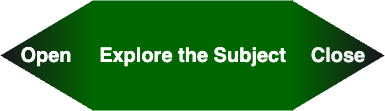
\includegraphics{assets/presentations/facilitation/fac-process.drawio.png}
\caption{Facilitation Process}
\end{figure}

\hypertarget{act-one}{%
\paragraph*{ACT ONE}\label{act-one}}
\addcontentsline{toc}{paragraph}{ACT ONE}

\begin{itemize}
\tightlist
\item
  Orient the group
\item
  Set the stage
\item
  Develop themes
\end{itemize}

\hypertarget{act-two}{%
\paragraph*{ACT TWO}\label{act-two}}
\addcontentsline{toc}{paragraph}{ACT TWO}

\begin{itemize}
\tightlist
\item
  Examine
\item
  Explore
\item
  Problem-solve
\end{itemize}

\hypertarget{act-three}{%
\paragraph*{ACT THREE}\label{act-three}}
\addcontentsline{toc}{paragraph}{ACT THREE}

\begin{itemize}
\tightlist
\item
  Plan
\item
  Decide
\item
  Conclude
\end{itemize}

\hypertarget{facilitating-the-process-of-prescribed-learning}{%
\subsubsection*{Facilitating the Process of Prescribed Learning}\label{facilitating-the-process-of-prescribed-learning}}
\addcontentsline{toc}{subsubsection}{Facilitating the Process of Prescribed Learning}

\[\text{Current Status}\Longrightarrow \Longrightarrow \Longrightarrow \Longrightarrow \text{Specific Goal}\]

\hypertarget{facilitating-the-process-of-inquiry-rich-learning}{%
\subsubsection*{Facilitating the Process of Inquiry-rich Learning}\label{facilitating-the-process-of-inquiry-rich-learning}}
\addcontentsline{toc}{subsubsection}{Facilitating the Process of Inquiry-rich Learning}

\[\text{Current Status} \curvearrowright \rightsquigarrow\nearrow\searrow\looparrowright\Updownarrow\rightrightarrows\text{Fuzzy Goal}\]

\hypertarget{managing-group-dynamics}{%
\subsubsection*{Managing Group Dynamics}\label{managing-group-dynamics}}
\addcontentsline{toc}{subsubsection}{Managing Group Dynamics}

\hypertarget{cohesion-factors-that-cultivate-predictable-trust}{%
\subsubsection*{Cohesion Factors that Cultivate (Predictable) Trust}\label{cohesion-factors-that-cultivate-predictable-trust}}
\addcontentsline{toc}{subsubsection}{Cohesion Factors that Cultivate (Predictable) Trust}

\begin{itemize}
\tightlist
\item
  Similarity. The more similar members are in terms of age, sex, education, skills, attitudes, values, and beliefs, the more likely the group will bond.
\item
  Stability. The longer a group stays together, the more cohesive it becomes.
\item
  Size. Smaller groups tend to have higher cohesion.
\item
  Support. Coaching and encouragement to support other members strengthens the group's identity.
\item
  Satisfaction. How pleased group members are with each other's performance, behaviour, and conformity to group norms increases cohesion.
\end{itemize}

\hypertarget{social-loafing}{%
\subsubsection*{Social Loafing}\label{social-loafing}}
\addcontentsline{toc}{subsubsection}{Social Loafing}

\begin{itemize}
\tightlist
\item
  There is a tendency of individuals to put in less effort when working in a group context.
\item
  As group size grows, this effect becomes larger.
\end{itemize}

\hypertarget{how-do-learning-groups-develop-over-time}{%
\subsubsection*{How do learning groups develop over time?}\label{how-do-learning-groups-develop-over-time}}
\addcontentsline{toc}{subsubsection}{How do learning groups develop over time?}

\begin{figure}
\centering
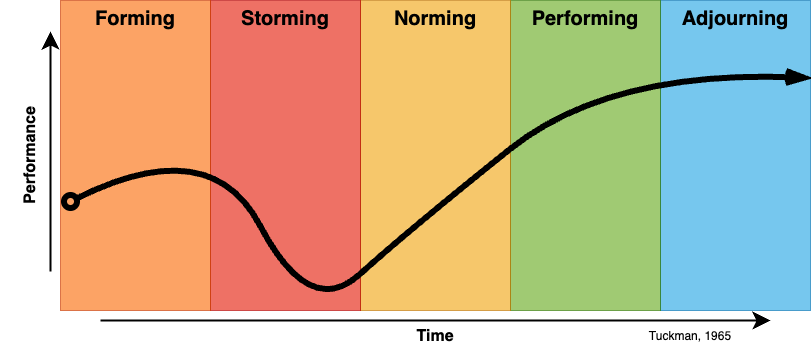
\includegraphics{assets/presentations/facilitation/tuckman.drawio.png}
\caption{Tuckman's Stages of Group Performance}
\end{figure}

\begin{itemize}
\tightlist
\item
  Forming: Learning group members get to know one another, exchange personal information, and establish new relationships.
\item
  Storming: Learning group members open up to each other and confront each other's ideas and perspectives.
\item
  Norming: Learning group members achieve a consensus about goals, definition of roles, and clear coordination of effort.
\item
  Performing: The learning group is able to function as a unit as they find ways to get the job done smoothly and effectively without inappropriate conflict or the need for external supervision.
\item
  Adjourning: admittedly a strained rhyme, but the idea, which is not in Tuckman's original model, is that the group will eventually disband, and it is important to finish well, gather data on the process, and carry forward lessons learned.
\end{itemize}

\begin{reflect}
\textbf{\emph{The life of learning groups is dynamic and cyclical.}}
\end{reflect}

\begin{figure}
\centering
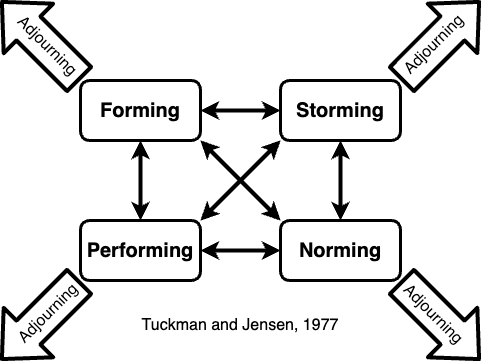
\includegraphics{assets/presentations/facilitation/tuckman-jensen.drawio.png}
\caption{Tuckman and Jensen's Stages of Group Performance}
\end{figure}

\hypertarget{tpr-life-cycle-model-white-2009}{%
\subsubsection*{TPR Life-cycle Model (White, 2009)}\label{tpr-life-cycle-model-white-2009}}
\addcontentsline{toc}{subsubsection}{TPR Life-cycle Model (White, 2009)}

\begin{longtable}[]{@{}ll@{}}
\toprule\noalign{}
Tuckman Model & TPR Model \\
\midrule\noalign{}
\endhead
\bottomrule\noalign{}
\endlastfoot
Forming & Transforming \\
Storming & - \\
Norming & - \\
Performing & Performing \\
Adjourning & Reforming \\
\end{longtable}

\begin{longtable}[]{@{}
  >{\centering\arraybackslash}p{(\columnwidth - 2\tabcolsep) * \real{0.6250}}
  >{\raggedright\arraybackslash}p{(\columnwidth - 2\tabcolsep) * \real{0.3750}}@{}}
\toprule\noalign{}
\begin{minipage}[b]{\linewidth}\centering
Developmental Phase (White, 2009)
\end{minipage} & \begin{minipage}[b]{\linewidth}\raggedright
Coaching and Facilitation Guidelines
\end{minipage} \\
\midrule\noalign{}
\endhead
\bottomrule\noalign{}
\endlastfoot
\textbf{Transforming} (Me to We) & \\
\emph{Forming} (Unwilling/unable) & Clear goals, \textbf{directions}, fairness, firmness (Why: overcoming denial of the new reality) \\
\emph{Storming} (Willing/unable) & As above, plus \textbf{encouraging participation}, calmness, recognition of concerns (Why: overcoming defence of the old reality) \\
\emph{Norming} (Unwilling/able) & Encouraging, \textbf{confidence building}, clear goals, holding accountable (Why: helping discard the old reality) \\
\textbf{Performing} (Willing/able) & Clear goal setting, monitoring, strategic preparation, seeking innovative approaches, \textbf{empowering team members} (Why: helping make new adaptations) \\
\textbf{Reforming} (Disengaging) & \textbf{Establishing new goals}, solving confusion, managing risks (Why: challenging the new comfort zone) \\
\end{longtable}

\hypertarget{learning-group-experience-punctuated-equilibrium}{%
\subsubsection*{Learning Group Experience Punctuated Equilibrium}\label{learning-group-experience-punctuated-equilibrium}}
\addcontentsline{toc}{subsubsection}{Learning Group Experience Punctuated Equilibrium}

\begin{figure}
\centering
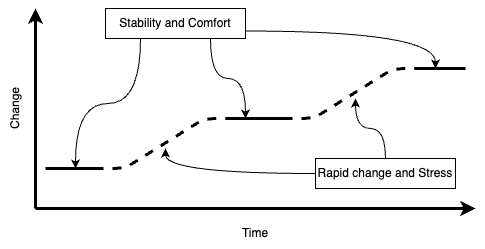
\includegraphics{assets/presentations/facilitation/pe.drawio.png}
\caption{Learning Group Experience Punctuated Equilibrium}
\end{figure}

\hypertarget{managing-the-group-learning-process}{%
\subsubsection*{Managing the group learning process}\label{managing-the-group-learning-process}}
\addcontentsline{toc}{subsubsection}{Managing the group learning process}

Working with Creative Tension in Teams

\begin{enumerate}
\def\labelenumi{\arabic{enumi}.}
\tightlist
\item
  be clear about the results the team wants to create (vision as important as group dynamics reality);
\item
  understand the underlying structural dynamics that influence the team's ability to create;
\item
  work on changing those underlying structures in order to bring the current reality in line with the desired outcome.
\end{enumerate}

\hypertarget{zone-of-proximal-development-1}{%
\subsubsection*{Zone of Proximal Development}\label{zone-of-proximal-development-1}}
\addcontentsline{toc}{subsubsection}{Zone of Proximal Development}

\begin{figure}
\centering
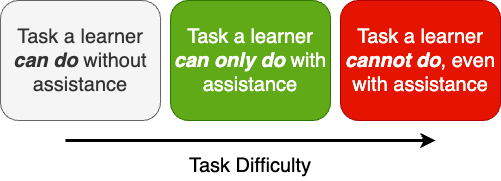
\includegraphics{assets/presentations/facilitation/zpd.drawio.png}
\caption{Zone of Proximal Development}
\end{figure}

\begin{figure}
\centering
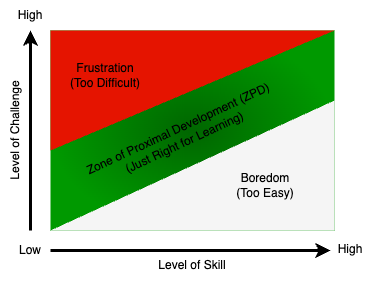
\includegraphics{assets/presentations/facilitation/zpd2.drawio.png}
\caption{Zone of Proximal Development}
\end{figure}

\hypertarget{scaffolding-1}{%
\subsubsection*{Scaffolding}\label{scaffolding-1}}
\addcontentsline{toc}{subsubsection}{Scaffolding}

\hypertarget{coaching-for-learning}{%
\chapter{Coaching for Learning}\label{coaching-for-learning}}

\hypertarget{overview-2}{%
\section*{Overview}\label{overview-2}}
\addcontentsline{toc}{section}{Overview}

An enduring principle of educational practice is learners learn in different ways and at different rates. Effective educators recognize the uniqueness of each individual learner. They understand each learner arrives at a new learning situation with different lived experiences, existing knowledge, cognitive processing strengths and weaknesses, learning preferences, values, and goals. At the same time, effective educators also recognize some aspects of the learning process are common to most, if not all, learners. For instance, most educators believe learning is an ongoing, reflective process. We tend to broadly believe human are constantly taking in new information, integrating it into what we already know, and developing ideas based on this merging of past and present. In the midst of educator's diverse and sometimes contradictory ideas about learning, there seems to be a great deal of mystery, and countless myths about how the learning process actually works. Unit 4 will introduce some important questions about learning, such as:

❓ How can we as educators ensure our students are truly achieving the outcomes we intend?\\
❓ What practises should educators use in order to create an effective learning environment?\\
❓ What role do learners play in generating and sustaining this environment?\\
❓ How can we maximize the likelihood of transformational learning?

\hypertarget{topics-2}{%
\subsection*{Topics}\label{topics-2}}
\addcontentsline{toc}{subsection}{Topics}

This unit is divided into the following topics:

\begin{enumerate}
\def\labelenumi{\arabic{enumi}.}
\tightlist
\item
  Theories of Learning (or \emph{What do we Really Know About How People Learn})
\item
  The Practice of Coaching
\item
  Core Coaching Competencies
\end{enumerate}

\hypertarget{learning-outcomes-2}{%
\subsection*{Learning Outcomes}\label{learning-outcomes-2}}
\addcontentsline{toc}{subsection}{Learning Outcomes}

When you have completed this unit, you should be able to:

\begin{itemize}
\tightlist
\item
  Describe theories about how people learn.
\item
  Explain how to design learning environments to maximize learning.
\item
  Explain the coaching for learning model.
\item
  Identify essential coaching for learning competencies.
\end{itemize}

\hypertarget{resources-3}{%
\subsection*{Resources}\label{resources-3}}
\addcontentsline{toc}{subsection}{Resources}

Online resources will be provided in the unit.

\href{https://ma-lead.github.io/ldrs663/coaching-notes.html}{Coaching Notes}

\hypertarget{topic-1-1}{%
\section*{Topic 1}\label{topic-1-1}}
\addcontentsline{toc}{section}{Topic 1}

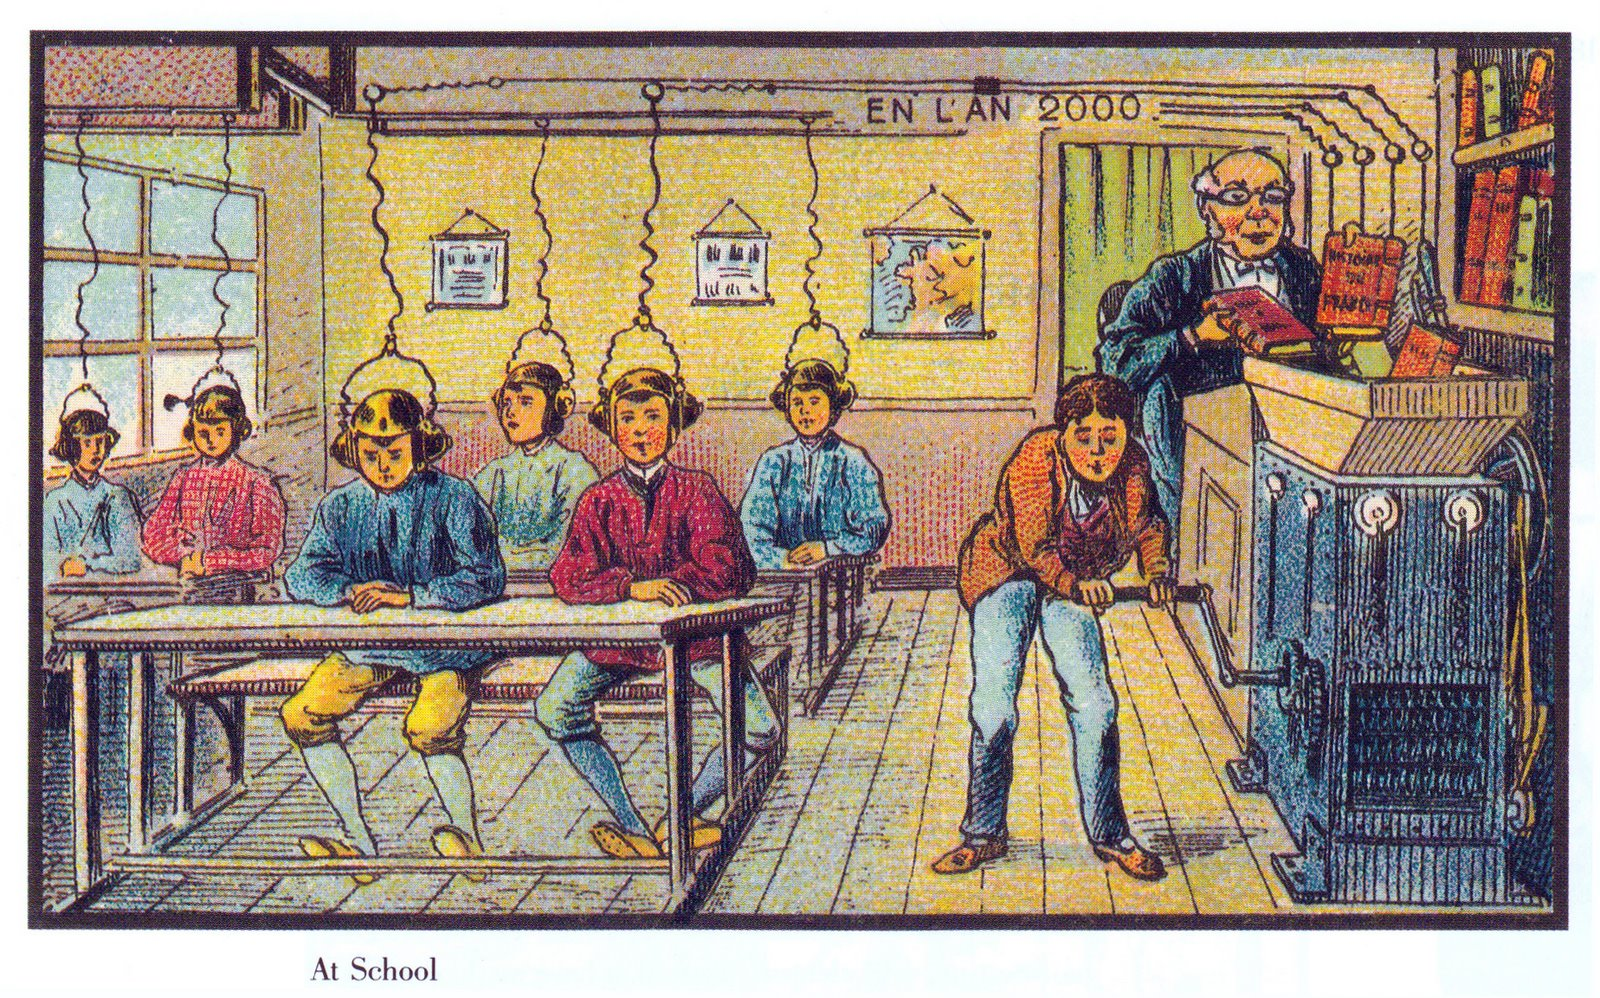
\includegraphics{assets/u4/France_in_XXI_Century._School.jpg}
\emph{This image is in the Public Domain.}

The image you see here was created in the early 20th century in France as a part of a series of images predicting what life would be like in 2000. You can see the full collection \href{https://publicdomainreview.org/collections/france-in-the-year-2000-1899-1910/}{\textbf{here}}.

As you can see, the artist envisioned a process whereby information was fed into a machine of some sort and just automagically downloaded into student minds. Kind of like this scene from the movie the \emph{Matrix}:

These are both examples of how the modern condition of thought (Unit 2), has shaped our thinking about learning. Many modern era educators viewed people as learning ``machines'' who could be ``programmed'' with instructions, just like we program computers. The legacy of this thinking still lingers and the educational model of instructors instructing students through instructions is still prevalent.

In these modern visions, learning is something done \emph{to} students, not something done \emph{by} students. The learner is completely passive in the process. The dreams of grade-schoolers to be able to rest a book on their head and learn by osmosis are just as far-fetched as the prognostications from the early 20th century, from the \emph{Matrix,} and from the claims of many edtech companies today. However, we need to recognize that learning is hard work. Consider Erasmus's (1965) comment in his dialogue \emph{The Art of Learning}, ``For my part, I know no other art of learning than hard work, devotion, and perseverance'' (p.~461). This statement remains as true today, as it was in 1529.

Take a few minutes to watch this video from Destin Sandlin, creator of the YouTube channel \emph{Smarter Every Day}. The video has a long introduction, but it is entertaining and sets up the problem of learning very well:

Destin talks about some important ideas related to pedagogy (the study of how children learn) that are also applicable to andragogy (the study of how adults learn). One of those ideas is that \emph{knowledge != understanding} (and now you know that the `!' negates the `=' in that statement). A little later in this unit, when we talk about deep and surface approaches to learning, we will come back to this idea.

\begin{reflect}
\hypertarget{reflect}{%
\subsubsection*{Reflect}\label{reflect}}
\addcontentsline{toc}{subsubsection}{Reflect}

As a way to consolidate your own learning around this concept, take a few minutes to think about a time when you have had knowledge, but not understanding, and how that affected you in some way. You don't have to write anything down, just connect the idea to an experience that you have had.
\end{reflect}

In the video, Destin also talks about cognitive bias and the tremendously powerful effect that our own biases have on what and how well we learn. The challenge that he faced in learning to ride the backwards brain bike wasn't so much the physical skills involved, but \emph{unlearning} his previous `ride a bike' algorithm. When he encountered new information that didn't match his previous experience, it was extremely difficult to overcome his previous experience and bias. It took him 8 months of dedicated effort to do it. At the end, he discovered that he hadn't \emph{overcome} his bias, he had only transferred it to a new bias, albeit one that was easier to overcome.

This process is also true for people learning new ideas. None of us come to a learning context without preconceived ideas regarding the nature of the topic to be studied, and often, those ideas are incorrect. They are misconceptions. Biases. Then, when new information comes along, our brain actively sabotages us by telling us that we already know this and we don't need to listen, while simultaneously convincing us even more of the truth of our misconceptions.

Below is another video, this time from \emph{Veritasium,} in which Derek Muller shows why misconceptions (biases) can be so difficult to overcome:

Despite the difficulty, it is important to note that we \emph{can} overcome these biases and misconceptions. In fact, we can overcome some bizarre inputs, as \href{https://www.theguardian.com/education/2012/nov/12/improbable-research-seeing-upside-down}{researchers have discovered and was briefly reported in The Guardian}.

Here is a slightly less scientifically rigorous portrayal of what happens when our vision is artificially flipped: (The video is 12 minutes, but you don't need to watch it all).

The point of these experiments, at least for our purposes, is that human brains (and likely other animals as well) demonstrate the characteristic of \emph{plasticity}. The connections in our brain that allow ideas to form and be adjusted can be broken and then reconnected in different configurations.

\textbf{\emph{This is learning. Learning is hard work.}}

One implication of this is that it is naïve for educators to assume that a single exposure to an idea will somehow cause learning. In fact, the opposite is true. It takes repeated exposure, practice, error-correction, and adjustment for learning to become consolidated.

\begin{reflect}
\hypertarget{read-and-reflect}{%
\subsubsection*{Read and Reflect}\label{read-and-reflect}}
\addcontentsline{toc}{subsubsection}{Read and Reflect}

Read Chapters 1-3 of How people learn II: Learners, Context and Cultures, \href{https://www.nap.edu/catalog/24783}{available for free download here}.

Note: We will not be using this entire book, so don't feel obliged to purchase a copy for yourself.
Click `Read Online' As you read, please use hypothes.is to both record your thoughts and connections in the article, but also interact with past annotations. These chapters are already heavily annotated, presumably by other students.

\textbf{\emph{Questions to Consider\ldots{}}}

After completing the reading above, consider the following questions:

\begin{itemize}
\tightlist
\item
  \emph{What are the basic types of learning?}
\item
  \emph{How does the human brain respond to learning?}
\end{itemize}
\end{reflect}

\begin{reflect}
\hypertarget{read-and-reflect-1}{%
\subsubsection*{Read and Reflect}\label{read-and-reflect-1}}
\addcontentsline{toc}{subsubsection}{Read and Reflect}

Below is a resource that summarizes existing research from cognitive science related to how students learn. This research has practical implications for teaching and learning that will be of benefit as we move forward with the content of this unit. Follow the link below:

\begin{itemize}
\tightlist
\item
  \href{https://deansforimpact.org/wp-content/uploads/2016/12/The_Science_of_Learning.pdf}{\textbf{The Science of Learning}}
\end{itemize}

\textbf{\emph{Questions to Consider\ldots{}}}

After completing the reading above, consider the following questions:

\begin{itemize}
\tightlist
\item
  \emph{How do students understand new ideas?}
\item
  \emph{How do students learn and retain new information?}
\item
  \emph{How do students solve problems?}
\item
  \emph{How does learning transfer to new situations in or outside of the classroom?}
\item
  \emph{What motivates students to learn?}
\item
  \emph{What are common misconceptions about how students think and learn?}
\end{itemize}
\end{reflect}

\hypertarget{topic-2-1}{%
\section*{Topic 2}\label{topic-2-1}}
\addcontentsline{toc}{section}{Topic 2}

\textbf{\emph{What is Coaching?}} Coaching is something that you do to help improve someone in some way. Gallway (1997) defines coaching as ``a way of being, listening, asking, and speaking that draws out and augments characteristics and potential that are already present in a person.'' His conceptualization of the method is analogous to Michelangelo's approach to sculpture. Michelangelo believed that ``every block of stone has a statue inside it and it's the task of the sculptor to discover it.'' Similarly, Gallway (1997) writes:

\begin{quote}
\emph{Coaches know that an oak tree already exists within an acorn. They have seen the one grow into the other, over time and under the right conditions, and are committed to providing those conditions to the best of their abilities. Successful coaches continually learn how best to ``farm'' the potential they are given to nurture.}
\end{quote}

\textbf{\emph{How do Educators Coach Learners for Learning?}} The beginning point of an effective coaching for learning practice as an educator is the coaching relationship. It's critical, according to Gallway (1997), for coaches to ``{[}create{]} a safe and challenging environment in which learning can take place.'' In the educator's role as coach, this relationship is a shared learning space where the educator enters the learners' internal dialogue with their learning experiences. Coaching work involves two aims,

\begin{itemize}
\tightlist
\item
  helping each learner become aware of their own potential, and,\\
\item
  helping learners remove any interference in realizing this potential.
\end{itemize}

In terms of coaching for learning we know that it is a natural aspect of our nature as human beings to learn. That is, it's something we simply do naturally. But, one thing that makes learning difficult is that our past learning gradually starts to interfere with our present and future learning.

Increasing learners' awareness of their own internal resistance to new learning is the primary theme of coaching for learning. Common obstacles to learning, according to Gallway (1997), include the learner's assumption that they already know what is being taught, the fear of being judged, doubt, and trying too hard to appear learned. In broader terms, Scharmer (2016) has identified the learners' internal \textbf{\emph{voice of judgement}} (VoJ), \textbf{\emph{voice of cynicism}} (VoC), and \textbf{\emph{voice of fear}} (VoF) as universal factors interfering with learning. The role of effective coaching is to help learners overcome these obstacles by opening their mind, emotions, and will to new possibilities. This work involves coaching learners through the transition of change---that is,
- letting go of what was,
- moving through the transition, and
- embracing a new beginning.

The secondary theme of coaching for learning is increasing learners' awareness of how they may best realize their potential capacity to learn anything which they set out to learn. This involves coaching learners in the learning process and helping them make it more effective and efficient. This practice builds on the notion of transforming the learners' natural learning process into a disciplined set of study skills. A helpful approach that educators can use to coach for learning potential is the GROW coaching model. This model is based on the coaching concepts pioneered by Gallway (1997) and developed at the McKinsey consulting firm in the 1980s and first published in 1992 by John Whitmore in his book \emph{Coaching for Performance}. The model is widely used in leadership and life coaching contexts. For educators concerned with coaching for learning, we can apply this model in the following way:

\begin{bonus}
\textbf{Goal Setting.} Helping learners clarify \textbf{what} they need and more importantly want to learn? \textbf{Why} they need and/or truly want to learn it? And \textbf{when} they need to, or genuinely want, to learn it? The coach, here, also helps learners see how their personal goals can align with prescribed learning outcomes.

\textbf{Reality Checking.} Helping learners identify what they already know? What they can already do? What they have already done? What's moving them towards their goal? And what's getting in the way?

\textbf{Option Exploring.} Helping learners identify the various options they have to move them toward their goals. Brainstorming what else they can do to achieve their goals? Assessing what are the benefits and weaknesses of the various options that they have identified?

\textbf{Will be Doing.} Helping learners choose which options to act on. Determining when to act on an option. Assessing how committed they are to taking action a given option? Committing to acting on an option.
\end{bonus}

\begin{reflect}
\hypertarget{read-and-reflect-2}{%
\subsubsection*{Read and Reflect}\label{read-and-reflect-2}}
\addcontentsline{toc}{subsubsection}{Read and Reflect}

Take a few moments to read the article below written by Tim Gallwey. Gallwey works with companies to help them find better ways to implement change. In the article below, he discusses the importance of creating a learning culture - specifically, he discusses why coaches need to understand the learning process and the obstacles a learner experiences:

\begin{itemize}
\tightlist
\item
  \href{https://thesystemsthinker.com/the-inner-game-of-work-building-capability-in-the-workplace/}{\textbf{The Inner Game of Work}}
\end{itemize}

\textbf{\emph{Questions to Consider\ldots{}}}

After completing the activity above, consider the following questions:

\begin{itemize}
\tightlist
\item
  \emph{How can coaching concepts be applied to helping learners learn?}
\item
  \emph{What key characteristics define effective coaching for learning?}
\item
  \emph{How can educators coach learners through the transition of making a change?}
\end{itemize}
\end{reflect}

\hypertarget{topic-3}{%
\section*{Topic 3}\label{topic-3}}
\addcontentsline{toc}{section}{Topic 3}

Effective coaching is grounded in an emerging set of coaching competencies. These competencies represent a set of integrated knowledge, skills, aptitudes and attributes that coalesce into behaviors that define, in more detail, what is needed to successfully perform the task of helping learners learn. The following are six essential behaviors the developing educator as coach must demonstrate.

\hypertarget{practicing-professional-ethics-standards}{%
\subsection*{\texorpdfstring{\textbf{Practicing Professional Ethics \& Standards}}{Practicing Professional Ethics \& Standards}}\label{practicing-professional-ethics-standards}}
\addcontentsline{toc}{subsection}{\textbf{Practicing Professional Ethics \& Standards}}

The basis of this competency is a personal commitment to demonstrating and maintaining the highest level of ethical behavior. Emerging professional coaching standards include,\\
✅ making the roles, responsibilities, and rights of everyone involved in the coaching relationship clear,\\
✅ clearly communicating how information will be communicated between everyone involved in the coaching relationship,\\
✅ maintain confidentiality of personal information and communications,\\
✅ having a clear understanding of the conditions where information will not be kept confidential, and\\
✅ be aware of and respond sensitively to potential power or status differences.

\hypertarget{cultivating-trust-safety}{%
\subsection*{Cultivating Trust \& Safety}\label{cultivating-trust-safety}}
\addcontentsline{toc}{subsection}{Cultivating Trust \& Safety}

Seeks to understand the learner and their unique learning context, demonstrates respect for the learner's identity, values and perspective, showing empathy and concern for their well-being, acknowledges the learner unique abilities, interests, and feelings, demonstrating openness and vulnerability, and supporting the unique needs of the learner's personality.

\hypertarget{holding-spacepresence}{%
\subsection*{Holding Space/Presence}\label{holding-spacepresence}}
\addcontentsline{toc}{subsection}{Holding Space/Presence}

Being focused on the moment and giving attention to what is occurring in your conversation with the learner. Initially, this might feel like simply holding yourself back from talking too much as the coach and giving the learner space (that is, your silence) to reflect and process things. One way to conceptualize this competency as ``creating a ``space to listen into.'' This involves\\
✅ creating comfortable distance in physical space,\\
✅ creating a non-judgmental emotional space, and\\
✅ creating a quiet auditory space. Holding space, or being present, is an essential way the educator as coach can demonstrate to the learner that the learner's contribution is valued and their learning is important. It's also important for the coach to hold space for themselves to reflect and process what is happening.

\hypertarget{active-listening}{%
\subsection*{Active Listening}\label{active-listening}}
\addcontentsline{toc}{subsection}{Active Listening}

The intent of these particular skills is to help the coach truly understand the learner and their context, and to help the learner feel like they have been understood and supported. Typical skills include, paying attention, holding judgement, reflecting, clarifying, summarizing, and sharing.

\hypertarget{evoking-awareness}{%
\subsection*{Evoking Awareness}\label{evoking-awareness}}
\addcontentsline{toc}{subsection}{Evoking Awareness}

Asks questions to clarify the learners' experiences, way of thinking, feelings, values, needs, wants, and beliefs. Asking questions to help learners explore beyond their current thinking. Invites learners to share more about their present learning experiences. Notices what is working to enhance the learners progress. Challenges learners to increase their awareness and insight. Helps learners identify their potential for growth, internal/external obstacles, and options to move forward. Shares observations, insights, and encouragements to assist the learner in their learning.

\hypertarget{cultivating-growth}{%
\subsection*{Cultivating Growth}\label{cultivating-growth}}
\addcontentsline{toc}{subsection}{Cultivating Growth}

Asks questions that helps learners\\
✅ surface their interests,\\
✅ clarify and prioritize their goals,\\
✅ assess their learning experiences,\\
✅ explore options for continued learning, and\\
✅ design learning plans and commit to achieving their learning goals.

\begin{reflect}
\hypertarget{read-and-reflect-3}{%
\subsubsection*{Read and Reflect}\label{read-and-reflect-3}}
\addcontentsline{toc}{subsubsection}{Read and Reflect}

For this activity, you will be reading through the Core Competencies of the International Coaching Federation. The International Coaching Federation is dedicated to advancing the coaching profession by setting high, ethical standards. Read more below:

\begin{itemize}
\tightlist
\item
  \href{https://coachfederation.org/core-competencies}{\textbf{Core Competencies}}
\end{itemize}

\textbf{\emph{Questions to Consider\ldots{}}}

After completing the activity above, consider the following questions:

\begin{itemize}
\tightlist
\item
  \emph{What general coaching competencies apply to coaching for learning?}
\item
  \emph{What competencies do you feel are strength areas? What areas do you need to develop?}
\item
  \emph{How can a coaching approach help you support learner success in an educational setting?}
\end{itemize}
\end{reflect}

\hypertarget{unit-4-assessment}{%
\section*{Unit 4 Assessment}\label{unit-4-assessment}}
\addcontentsline{toc}{section}{Unit 4 Assessment}

\begin{wp}
\hypertarget{wordpress-post-1}{%
\subsubsection*{WordPress Post}\label{wordpress-post-1}}
\addcontentsline{toc}{subsubsection}{WordPress Post}

Please complete the assignment under `Post 3' below. This will be your third of four draft posts during the course.

\href{https://ma-lead.github.io/ldrs663/assessments.html\#post-3}{Blog Post 3}

In addition, please begin planning your \href{https://ma-lead.github.io/ldrs663/assessments.html\#peer-coaching-session-15}{Peer Coaching Session}.
\end{wp}

\begin{feedback}
\hypertarget{things-to-do-this-week}{%
\subsubsection*{Things To Do This Week}\label{things-to-do-this-week}}
\addcontentsline{toc}{subsubsection}{Things To Do This Week}

✅ Meet in Zoom {Wednesday, October 4 - 10:30 AM PDT}\href{https://www.timeanddate.com/worldclock/fixedtime.html?msg=LDRS663+Meeting\&iso=20231004T1030\&p1=1109\&ah=1}{Check your local time here}
✅ Meet in Zoom {Wednesday, October 11 - 10:30 AM PDT}\href{https://www.timeanddate.com/worldclock/fixedtime.html?msg=LDRS663+Meeting\&iso=20231011T1030\&p1=1109\&ah=1}{Check your local time here}\\
✅ \textbf{Read} and \textbf{Reflect} Chapters 1-3 of How people learn II: Learners, Context and Cultures, \href{https://www.nap.edu/catalog/24783}{available for free download here}.\\
✅ \textbf{Read} and \textbf{Reflect} \href{https://deansforimpact.org/wp-content/uploads/2016/12/The_Science_of_Learning.pdf}{\textbf{The Science of Learning}}\\
✅ \textbf{Read} and \textbf{Reflect} \href{https://thesystemsthinker.com/the-inner-game-of-work-building-capability-in-the-workplace/}{\textbf{The Inner Game of Work}}\\
✅ \textbf{Read} and \textbf{Reflect} \href{https://coachfederation.org/core-competencies}{\textbf{Core Competencies}}\\
✅ \textbf{Publish} your \href{https://ma-lead.github.io/ldrs663/assessments.html\#post-3}{Unit 3 Post} using the category \texttt{ldrs663}.\\
✅ \textbf{Meet} with your Learning Pod to complete the \href{https://ma-lead.github.io/ldrs663/assessments.html\#peer-coaching-session}{Peer Coaching Session}.
✅ Please complete these items by {Saturday, October 14 - by sundown}, or let me know if you will need a bit more time.
\end{feedback}

\hypertarget{coaching-notes}{%
\chapter*{Coaching Notes}\label{coaching-notes}}
\addcontentsline{toc}{chapter}{Coaching Notes}

\hypertarget{what-is-coaching}{%
\subsubsection*{\texorpdfstring{What is \textbf{coaching}?}{What is coaching?}}\label{what-is-coaching}}
\addcontentsline{toc}{subsubsection}{What is \textbf{coaching}?}

\begin{quote}
Coaching is a way of being, listening, asking, and speaking that draws out and augments characteristics and potential that are already present in a person. \textasciitilde Gallwey, 1997
\end{quote}

\hypertarget{michaelangelos-principle}{%
\subsubsection*{Michaelangelo's Principle}\label{michaelangelos-principle}}
\addcontentsline{toc}{subsubsection}{Michaelangelo's Principle}

\begin{quote}
Every block of stone has a statue inside it and it is the task of the sculptor to discover it.''
\end{quote}

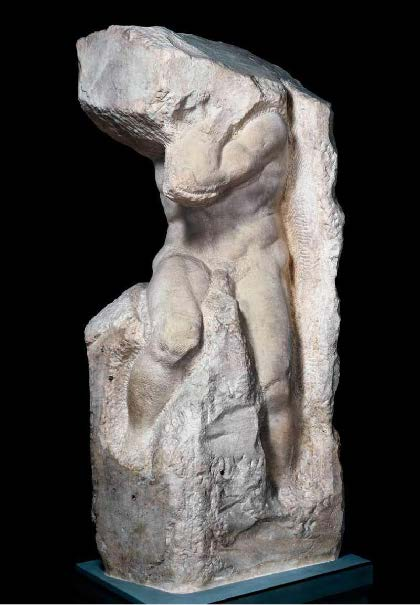
\includegraphics{assets/presentations/coaching/mike.jpg}

\hypertarget{developing-learning-capability}{%
\subsubsection*{Developing Learning Capability}\label{developing-learning-capability}}
\addcontentsline{toc}{subsubsection}{Developing Learning Capability}

\begin{itemize}
\tightlist
\item
  Learning, coaching, and building a learning culture are critical to the multi-access education model.
\item
  Growing learners' learning capability is equivalent to increasing an institution's teaching presence.
\item
  We don't really need to learn how to learn; we need to remove our resistance to learning and coaching.
\end{itemize}

\hypertarget{aims-of-coaching-for-learning}{%
\subsubsection*{Aims of coaching for Learning}\label{aims-of-coaching-for-learning}}
\addcontentsline{toc}{subsubsection}{Aims of coaching for Learning}

\begin{itemize}
\tightlist
\item
  Increase capacity for learning performance:

  \begin{itemize}
  \tightlist
  \item
    by actualizing potential;
  \item
    or, by decreasing interference;
  \item
    or, by a combination of both.
  \end{itemize}
\end{itemize}

\hypertarget{learning-performance-potential---interference}{%
\subsubsection*{Learning Performance = Potential - Interference}\label{learning-performance-potential---interference}}
\addcontentsline{toc}{subsubsection}{Learning Performance = Potential - Interference}

\textasciitilde Gallwey, 1997

\hypertarget{core-coaching-competencies}{%
\subsubsection*{Core Coaching Competencies}\label{core-coaching-competencies}}
\addcontentsline{toc}{subsubsection}{Core Coaching Competencies}

\begin{itemize}
\tightlist
\item
  Practicing Professional Ethics \& Standards
\item
  Cultivating Trust \& Safety
\item
  Holding Space/ Presence
\item
  Active Listening
\item
  Asking Questions
\item
  Creating Awareness
\item
  Setting (SMART) Goals
\item
  Designing Action Plans
\item
  Checking for Results
\end{itemize}

\hypertarget{listening}{%
\subsubsection*{Listening}\label{listening}}
\addcontentsline{toc}{subsubsection}{Listening}

The reality is that

\begin{quote}
``to {[}truly{]} listen is very hard, because it asks of us so much interior stability that we no longer need to prove ourselves by speeches, arguments, statements or declarations. True listeners no longer have an inner need to make their presence known. They are free to receive, welcome, to accept''.
\textasciitilde Henri Nouwen
\end{quote}

\hypertarget{levels-of-listening}{%
\subsubsection*{Levels of Listening}\label{levels-of-listening}}
\addcontentsline{toc}{subsubsection}{Levels of Listening}

\begin{itemize}
\tightlist
\item
  Avoidance Listening = \textbf{Listening Over}
\item
  Defensive Listening = \textbf{Listening At}
\item
  Problem-Solving Listening = \textbf{Listening To}
\item
  Listening to Learn = \textbf{Listening Into}
  \textasciitilde Goulston \& Ullmen (2013)
\end{itemize}

\begin{reflect}
Why is ``listening into'' the inner world of the learner's lived-experience so difficult?
\end{reflect}

\hypertarget{reason-we-listen-autobiographically}{%
\subsubsection*{Reason: We listen autobiographically}\label{reason-we-listen-autobiographically}}
\addcontentsline{toc}{subsubsection}{Reason: We listen autobiographically}

\begin{itemize}
\item
  We listen with the intent to reply, not to understand what the other person is trying to say.
\item
  We listen to our own self-talk as we prepare what we are going to say, ask, etc.
\item
  We filter everything we hear through our life experiences, our own frame of reference.
\item
  We check what we hear against our own autobiography and see how it measures up.
\item
  We decide what the other person means before he/
  she finishes communicating, saying things like:

  \begin{itemize}
  \tightlist
  \item
    ``I know just how you feel.''
  \item
    ``I felt the same way.''
  \item
    ``I had that same thing happen to me.''
  \item
    ``Let me tell you what I did in a similar situation.''
  \end{itemize}
\end{itemize}

\hypertarget{other-common-barriers-to-effective-listening}{%
\subsubsection*{Other Common Barriers to Effective Listening}\label{other-common-barriers-to-effective-listening}}
\addcontentsline{toc}{subsubsection}{Other Common Barriers to Effective Listening}

\begin{itemize}
\tightlist
\item
  We see silence as agreement
\item
  We feel the pressure of time (we don't have time)
\item
  We are impatient/disinterested
\item
  We lack of know-how
\item
  We simply don't pay close attention
\end{itemize}

\hypertarget{we-need-to-learn-to-listen-into-learners-worlds-consciously}{%
\subsubsection*{We Need to Learn to ``Listen Into'' Learner's Worlds Consciously}\label{we-need-to-learn-to-listen-into-learners-worlds-consciously}}
\addcontentsline{toc}{subsubsection}{We Need to Learn to ``Listen Into'' Learner's Worlds Consciously}

\hypertarget{julian-treasure-2011-provides-us-with-critical-insights-into-how-we-can-listen-consciously.}{%
\subsubsection*{Julian Treasure (2011) provides us with critical insights into how we can listen consciously.}\label{julian-treasure-2011-provides-us-with-critical-insights-into-how-we-can-listen-consciously.}}
\addcontentsline{toc}{subsubsection}{Julian Treasure (2011) provides us with critical insights into how we can listen consciously.}

\begin{figure}
\centering
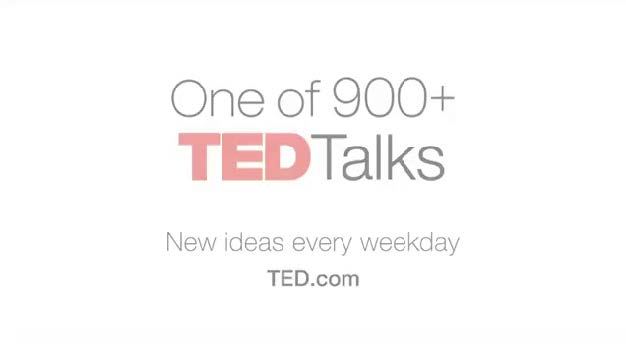
\includegraphics{assets/presentations/coaching/ted.jpg}
\caption{alt-text}
\end{figure}

\hypertarget{how-can-we-listen-consciously-to-our-learners-inner-worlds-to-truly-understand-them}{%
\subsubsection*{How can we listen consciously to our learners' inner world's to truly understand them?}\label{how-can-we-listen-consciously-to-our-learners-inner-worlds-to-truly-understand-them}}
\addcontentsline{toc}{subsubsection}{How can we listen consciously to our learners' inner world's to truly understand them?}

\hypertarget{our-listening-positions-need-to-match-the-situation}{%
\subsubsection*{Our Listening Positions Need to Match the Situation}\label{our-listening-positions-need-to-match-the-situation}}
\addcontentsline{toc}{subsubsection}{Our Listening Positions Need to Match the Situation}

\begin{itemize}
\tightlist
\item
  Active vs.~Passive
\item
  Reductive vs.~Expansive
\item
  Critical vs.~Empathetic
\end{itemize}

\hypertarget{coaching-for-learning-requires-active-listening}{%
\subsubsection*{Coaching for learning requires Active Listening}\label{coaching-for-learning-requires-active-listening}}
\addcontentsline{toc}{subsubsection}{Coaching for learning requires Active Listening}

\begin{figure}
\centering
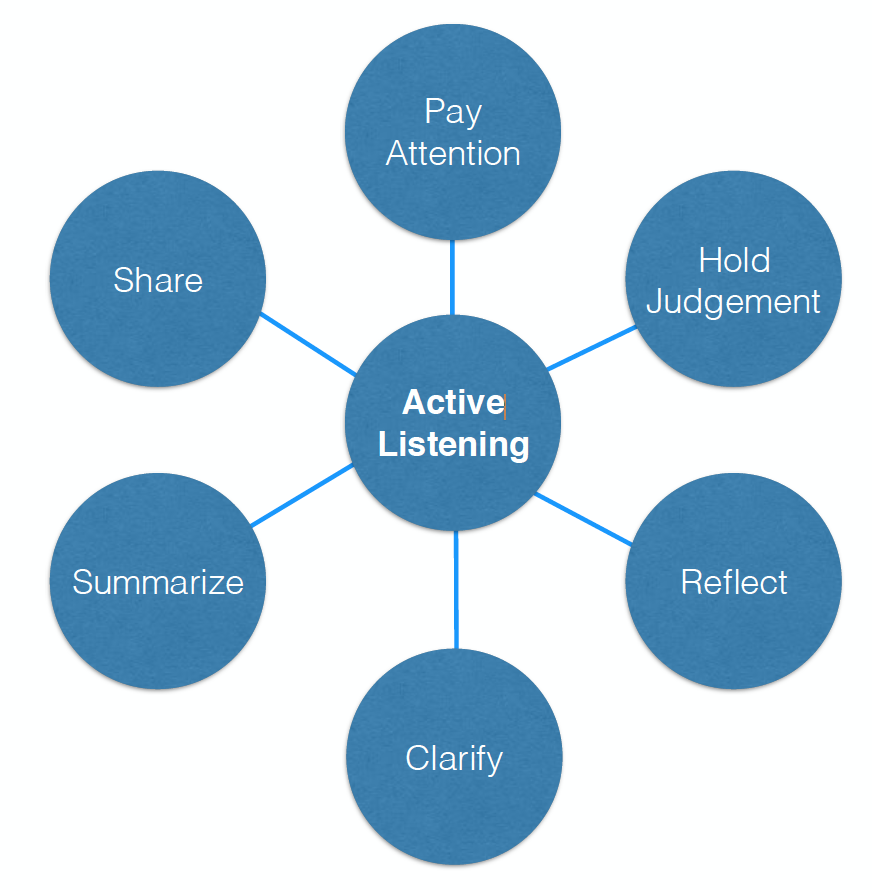
\includegraphics{assets/presentations/coaching/active.png}
\caption{alt-text}
\end{figure}

\hypertarget{pay-attention}{%
\subsubsection*{Pay Attention}\label{pay-attention}}
\addcontentsline{toc}{subsubsection}{Pay Attention}

\begin{enumerate}
\def\labelenumi{\arabic{enumi}.}
\tightlist
\item
  Be present; focus on the moment
\item
  Observe body language; your own and the learner's.
\item
  Pre-empt distractions.
\end{enumerate}

\hypertarget{hold-judgement}{%
\subsubsection*{Hold Judgement}\label{hold-judgement}}
\addcontentsline{toc}{subsubsection}{Hold Judgement}

\begin{enumerate}
\def\labelenumi{\arabic{enumi}.}
\tightlist
\item
  Practice empathy; seeking to make the learner ``feel'' felt and heard.
\item
  Try to understand learner's ``lens''.
\item
  Be patient.
\end{enumerate}

\begin{quote}
Silence is a source of great strength.
\textasciitilde Lao Tzu
\end{quote}

\hypertarget{reflect-1}{%
\subsubsection*{Reflect}\label{reflect-1}}
\addcontentsline{toc}{subsubsection}{Reflect}

\begin{enumerate}
\def\labelenumi{\arabic{enumi}.}
\tightlist
\item
  Paraphrase (``What I am hearing is\ldots{}'')
\item
  Name emotions you observe
\item
  Be a ``mirror''
\end{enumerate}

\begin{figure}
\centering
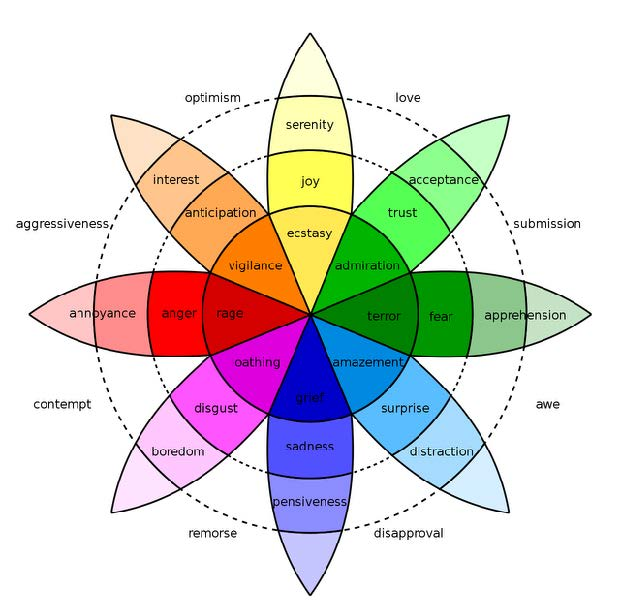
\includegraphics{assets/presentations/coaching/plutchik.jpg}
\caption{alt-text}
\end{figure}

\hypertarget{clarify}{%
\subsubsection*{Clarify}\label{clarify}}
\addcontentsline{toc}{subsubsection}{Clarify}

\begin{enumerate}
\def\labelenumi{\arabic{enumi}.}
\tightlist
\item
  Use open-ended questions (``What might you do next?).
\item
  Use clarifying questions (``Let me see, if I'm clear?'').
\item
  Use probing questions (``What tactics have you tried?'').
\end{enumerate}

\hypertarget{summarize}{%
\subsubsection*{Summarize}\label{summarize}}
\addcontentsline{toc}{subsubsection}{Summarize}

\begin{enumerate}
\def\labelenumi{\arabic{enumi}.}
\tightlist
\item
  Use ``So'' periodically (``So, what I have heard so far\ldots{}'').
\item
  Use ``So'' at the end (So, let me summarize what I have heard\ldots'').
\item
  Ask the other person to summarize.
\end{enumerate}

\hypertarget{share}{%
\subsubsection*{Share}\label{share}}
\addcontentsline{toc}{subsubsection}{Share}

\begin{enumerate}
\def\labelenumi{\arabic{enumi}.}
\tightlist
\item
  Be an active participant in the conversation.
\item
  Share thoughts, feelings, and experiences to deepen and/or check for understanding.
\item
  Ask the learner about your impact on him or her.
\end{enumerate}

\hypertarget{g.r.o.w.-coaching-model}{%
\subsubsection*{G.R.O.W. Coaching Model}\label{g.r.o.w.-coaching-model}}
\addcontentsline{toc}{subsubsection}{G.R.O.W. Coaching Model}

\hypertarget{goal-setting}{%
\section*{Goal Setting}\label{goal-setting}}
\addcontentsline{toc}{section}{Goal Setting}

\begin{itemize}
\tightlist
\item
  Setting short and long term learning goals.
\item
  Key questions to ask:

  \begin{itemize}
  \tightlist
  \item
    What can you do with my time that is important?
  \item
    What learning outcome do you want?
  \item
    How much time do you need to achieve that outcome?
  \item
    How does what you am doing now help you achieve the longer term learning outcomes I really want?
  \end{itemize}
\end{itemize}

\hypertarget{make-your-goals-s.m.a.r.t.}{%
\paragraph*{Make Your Goals S.M.A.R.T.}\label{make-your-goals-s.m.a.r.t.}}
\addcontentsline{toc}{paragraph}{Make Your Goals S.M.A.R.T.}

\hypertarget{specific}{%
\subparagraph*{Specific}\label{specific}}
\addcontentsline{toc}{subparagraph}{Specific}

\begin{itemize}
\tightlist
\item
  Your goal should be clear and specific.
\item
  Ask yourself:

  \begin{itemize}
  \tightlist
  \item
    What do I want to accomplish in this course?
  \item
    Why is this learning goal important to you?
  \item
    What is involved in achieving this goal?
  \end{itemize}
\end{itemize}

\hypertarget{measurable}{%
\subparagraph*{Measurable}\label{measurable}}
\addcontentsline{toc}{subparagraph}{Measurable}

\begin{itemize}
\tightlist
\item
  You should be able to track your progress.
\item
  Ask yourself:

  \begin{itemize}
  \tightlist
  \item
    How much time is involved?
  \item
    How will you know when it is accomplished?
  \end{itemize}
\end{itemize}

\hypertarget{attainable}{%
\subparagraph*{Attainable}\label{attainable}}
\addcontentsline{toc}{subparagraph}{Attainable}

\begin{itemize}
\tightlist
\item
  Your goal should be realistic and achievable.
\item
  Ask yourself:

  \begin{itemize}
  \tightlist
  \item
    How can you accomplish this goal?
  \item
    Do you have the resources to achieve it?
  \end{itemize}
\end{itemize}

\hypertarget{relevant}{%
\subparagraph*{Relevant}\label{relevant}}
\addcontentsline{toc}{subparagraph}{Relevant}

\begin{itemize}
\tightlist
\item
  Your goal should matter and align with your other
  goals.
\item
  Ask yourself:

  \begin{itemize}
  \tightlist
  \item
    Is the goal worthwhile?
  \item
    Is the time right?
  \item
    Does it help you achieve what you ultimately want?
  \end{itemize}
\end{itemize}

\hypertarget{time-bound}{%
\subparagraph*{Time-bound}\label{time-bound}}
\addcontentsline{toc}{subparagraph}{Time-bound}

\begin{itemize}
\tightlist
\item
  Your goal should have a deadline to focus on.
\item
  Ask yourself:

  \begin{itemize}
  \tightlist
  \item
    When?
  \item
    What can I do now?
  \end{itemize}
\end{itemize}

\hypertarget{reality-checking}{%
\section*{Reality Checking}\label{reality-checking}}
\addcontentsline{toc}{section}{Reality Checking}

\begin{itemize}
\tightlist
\item
  Understanding where you really are relative to what
  you really want.
\item
  Key questions to ask:

  \begin{itemize}
  \tightlist
  \item
    What is really going on?
  \item
    What have you done/tried?
  \item
    Have you noticed any patterns?
  \item
    How do you know this is accurate?
  \end{itemize}
\end{itemize}

\hypertarget{identifying-obstacles-to-achieving-goals}{%
\subsubsection*{Identifying Obstacles to Achieving Goals}\label{identifying-obstacles-to-achieving-goals}}
\addcontentsline{toc}{subsubsection}{Identifying Obstacles to Achieving Goals}

\begin{itemize}
\tightlist
\item
  Critical to identify if there's more than one obstacle.
\item
  Key questions to ask:

  \begin{itemize}
  \tightlist
  \item
    What is preventing you from achieving your goals?
  \item
    What else is preventing you?
  \item
    What do you have to change about yourself to achieve your goals?
  \item
    What is preventing you from changing?
  \end{itemize}
\end{itemize}

\hypertarget{common-obstacles-to-learning-goals}{%
\subsubsection*{Common Obstacles to Learning Goals}\label{common-obstacles-to-learning-goals}}
\addcontentsline{toc}{subsubsection}{Common Obstacles to Learning Goals}

\begin{itemize}
\tightlist
\item
  Assumption that ``I already know''
\item
  Assumption that learning means remediation
\item
  Fear of being judged
\item
  Doubt
\item
  Trying too hard to learn and to appear learned
  \textasciitilde Gallwey, 1997
\end{itemize}

\hypertarget{option-exploration}{%
\section*{Option Exploration}\label{option-exploration}}
\addcontentsline{toc}{section}{Option Exploration}

\begin{itemize}
\tightlist
\item
  Key questions to ask:

  \begin{itemize}
  \tightlist
  \item
    What alternatives do you have?
  \item
    Who can support you?
  \item
    What are the pros and cons of that option?
  \item
    What is the preferred option you want to act on?
  \end{itemize}
\end{itemize}

\hypertarget{reframing-questions}{%
\subsubsection*{Reframing Questions}\label{reframing-questions}}
\addcontentsline{toc}{subsubsection}{Reframing Questions}

\begin{itemize}
\tightlist
\item
  What are you not seeing?
\item
  What is a better position to take?
\item
  Is this problem the root problem or a symptom of it?
\item
  Why is this problem problematic?
\end{itemize}

\hypertarget{the-way-forward}{%
\section*{The Way Forward}\label{the-way-forward}}
\addcontentsline{toc}{section}{The Way Forward}

\begin{itemize}
\tightlist
\item
  Key questions to ask:

  \begin{itemize}
  \tightlist
  \item
    What commitments am I going to make?
  \item
    What are my next steps?
  \item
    In what timeframe?
  \item
    What do I think might get in the way?
  \item
    How will I track my progress?
  \item
    What support do I need? How will I get it?
  \end{itemize}
\end{itemize}

\hypertarget{creating-action-strategies}{%
\subsubsection*{Creating Action Strategies}\label{creating-action-strategies}}
\addcontentsline{toc}{subsubsection}{Creating Action Strategies}

\begin{itemize}
\tightlist
\item
  Set SMART Goal(s) (the job to be done)
\item
  Breakdown the Work (into a list of tasks)
\item
  Define the Critical Path (the order of tasks)
\item
  Schedule the Work (when you do what)
\end{itemize}

\hypertarget{building-the-web}{%
\chapter{Building the Web}\label{building-the-web}}

\hypertarget{overview-3}{%
\section*{Overview}\label{overview-3}}
\addcontentsline{toc}{section}{Overview}

This week, we will introduce you to some background thinking about educational technologies. There are countless companies vying for attention in the edtech field, and they are not all educationally beneficial. In fact, some are outright harmful. We believe that it is important for you to begin to think about how your data are used when you interact with edtech tools and that it is important for you to develop some skills and competencies in building your own domain on the web. With this knowledge, you will be more prepared to spot the nefarious actors and to take control of how you present yourself online.

\hypertarget{topics-3}{%
\section*{Topics}\label{topics-3}}
\addcontentsline{toc}{section}{Topics}

\begin{enumerate}
\def\labelenumi{\arabic{enumi}.}
\tightlist
\item
  Situating yourself online
\item
  Data and Privacy
\item
  Subverting surveilance capitalism
\end{enumerate}

\hypertarget{outcomes}{%
\section*{Outcomes}\label{outcomes}}
\addcontentsline{toc}{section}{Outcomes}

\begin{itemize}
\tightlist
\item
  you will be able to articulate the importance of data and your privacy rights\\
\item
  you will have gained confidence in presenting your whole self online\\
\item
  you will be able to create and manage a single WordPress blog.
\end{itemize}

\hypertarget{resources-4}{%
\section*{Resources}\label{resources-4}}
\addcontentsline{toc}{section}{Resources}

Online resources will be provided.

\hypertarget{visitors-and-residents}{%
\section{Visitors and Residents}\label{visitors-and-residents}}

It is likely that you have encountered and may believe that there is a distinction between digital `natives' and `immigrants'.

\begin{caution}
\textbf{Note}\\
\href{https://marcprensky.com/}{Marc Prensky}, who proposed this idea, is the one who thought it would be a good idea to refer to people as `natives'. We recognize that this term should not be used to talk about people.
\end{caution}

The essential argument is that \emph{kids these days} have changed in that they have this innate ability to use and learn technology because they have grown up using technology, and those of us whose formative years pre-date the advent of the internet are forever at a disadvantage compared to the \emph{kids}. You can read a bit more about the idea on Wikipedia, linked below. There is also a link in that article to Prensky's original article.

Digital native

Aside from the problematic framing of learners as kids, there are some distinct challenges with the idea of digital literacy being a fixed trait rather than a matter of comfort, familiarity, and a skill that can be practiced and learned. It is no secret that more young people are comfortable using social media apps like TikTok, Instagram, SnapChat, Weibo, WeChat, and the like, but that does not mean that those people are more able to learn technology than older people or that they have an innate ability to do so. Have you ever asked a 1st-year university student to use a spreadsheet to create a budget or a gradebook with embedded formulae? It is more likely than not, that you will encounter a distinct lack of skill in completing this task.

I'd like to introduce you to a different way to conceptualize your relationship with digital media, and that is that you may be a \emph{visitor} in some web spaces and a \emph{resident} in others. Places on the web where you might be a visitor are those places where you, quite literally, visit, but importantly, don't leave a public trace of your time there. You don't spend any time interacting with people, but rather, you take a rather utilitarian approach by visiting a site, doing a thing, and leaving.

Alternately, there are places and spaces on the web, where \emph{you} reside as a persona, where you interact, socialize, and leave traces of yourself online. For some, that may be Facebook, where you keep in touch with friends and family, or Twitter, or maybe it's a listserv you subscribed to back in the 90s, or your blog, or someone else's blog or social site. The important distinction is that these are places where you connect with other people; where you are socially \emph{present}.

At the same time, if we can imagine the visitor \textless--\textgreater{} resident continuum on a horizontal axis, there is also a personal \textless--\textgreater{} professional (or educational) continuum on a vertical axis, leading to 4 quadrants where you might situate your technology use.

The video below explains a process to help you think about where you reside on the web (7 mins).

\href{https://www.youtube.com/watch?v=sPOG3iThmRI}{Link to YouTube}

I've shared my VR Diagram below\ldots keep in mind that this diagram represents a set of tools that I have been using for a decade or more and that I have invested my career in educational technology. There is a lot here, but yours might look significantly different with only a few tools here and there. The main thing I would like to communicate with this idea of visitors and residents is for you to think about which technologies you use as a resident, and then to think about where your learners reside on the web. From there, we can begin to plan for tools we can use that afford us and our learners the opportunity to reside there.

\begin{figure}
\centering
\includegraphics{assets/u1/vr-diagram-2.png}
\caption{Visitor-Resident Diagram}
\end{figure}

It is certainly notable that I am very much a visitor in Moodle! This does not mean that I don't spend much time there, I spend a significant portion of every day working in Moodle, rather, the work that I do there leaves very little trace of my personality. You will (hopefully) see Moodle as much more of a place where you reside. But this foregrounds the question of whether Moodle is actually designed to promote residencies. Certainly the forums allow for users to project their persona into the system, as do a few of the other features, but the system itself is very heavily templated. There are profiles that can be edited, but users are limited to one very tiny image and virtually no opportunity to determine for themselves what they want to share. There is little room for customization, and every time a course ends, every single user must recreate their persona in a new course site (or five).

For many, or most, of you, Moodle is a perfectly reasonable place to reside and you are able to make learners feel at home there. We encourage that. And just like our physical homes, the quality of the community that lives there isn't determined by the features of the house itself, but by the people who share the space and how they structure their time and interactions.

If you don't already, I encourage you to subscribe to this excellent podcast called \emph{Teaching in Higher Ed} by \href{https://twitter.com/bonni208}{Bonni Stachowiak}, or, just take 47 minutes to listen to this episode in which Bonni interviews Dave White about the idea of visitors and residents.

Digital Visitors and Residents, with David White - Teaching in Higher Ed

One of the people I look up to as an educator published a blog post which I believe provides a fitting summary of this particular unit.

Technology is not Pedagogy

\hypertarget{learning-activity-9}{%
\subsection*{Learning Activity}\label{learning-activity-9}}
\addcontentsline{toc}{subsection}{Learning Activity}

\begin{wp}
\textbf{Visitor and Resident Diagram}

I hope this activity will help you think about how the tools we use shape and sometimes determine the nature of our interactions with learners. Do the tools you use fall on the visitor or the resident end of your continuum? What about the learners in your classes?

✔️ \textbf{Read} \href{https://firstmonday.org/ojs/index.php/fm/article/view/3171}{Visitors and Residents: A new typology for online engagement}\\
✔️ Complete your own \textbf{\emph{Visitor/Resident}} map and share and discuss it with your Learning Pod. You can use the \href{https://experimental.worldcat.org/vandrmapping/editMap}{tool that is provided here (DON'T forget to screenshot it, or you'll lose it!)}, or use a different tool like \href{https://canva.com}{Canva.com}.\\
✔️ Share your Visitor-Resident Diagram in a new post on your WordPress blog. Include a short reflection on what your diagram tells you about your web presence. Feel free to interact with others' diagrams!
\end{wp}

\hypertarget{fippa-privacy-and-consent-resources}{%
\section{FIPPA, Privacy, and Consent Resources}\label{fippa-privacy-and-consent-resources}}

It is second nature to most to take selfies and share them on Instagram, Snapchat, etc., but once you move into the role of an educator in either a public or private context, you must adhere to the laws set out by the \href{https://www.oipc.bc.ca/}{B.C. Office of Information and Privacy Commissioner}. Their office has put together guidelines for both public bodies and private bodies. TWU, as a private body is not held to the same standard as public bodies, but we should strive to meet the same standard. The guidelines for public bodies to better understand what the rules are is linked below and how to get consent is detailed on page 4 of the \href{https://esquimalt.public.sd61.bc.ca/wp-content/uploads/sites/34/2013/09/OIPC-Cloud-Computing-Guidelines-for-Public-Bodies.pdf}{BC Cloud Computing Guidelines (PDF)} and you can review the \href{http://www.bclaws.ca/Recon/document/ID/freeside/96165_00}{Freedom of Information and Protection of Privacy Act here.}. \href{https://www.twu.ca/about/university-privacy-policy}{TWU also has a privacy policy, available here.}

Each public body will have their own process (which may range from not allowing tools to pressure to integrate networked learning tools from outside of Canada), so it is important to understand your own setting and the law. You may find some administrators or staff breaking these rules or not aware of them. It is important for you to enter your field and uphold the law, regardless of the culture you enter. This does not mean that you do not engage online or outside of Canada. It means that if/when you do so, that you understand the steps, which are not much more complex than the consent you would get normally for going ``on the Internet,'' as is described in most settings, but you must name the date consent is effective and, if applicable, the date it expires. It is important that you work with your school district on the consent process. You can see an example of how K-12 school districts are addressing access to cloud tools outside of Canada \href{http://www.sd43.bc.ca/Resources/DigitalCitizenship/Pages/CloudTools.aspx}{here (Coquitlam)} and \href{https://www.sd61.bc.ca/programs/digital-learning/sd61-gafe/privacy-and-personal-information/}{here} plus \href{https://techforlearning.sd61.bc.ca/privacy/consent-process/}{here (Victoria)}. You must also name each tool individually. It cannot be ``blogging.'' You must name WordPress.com or Blogger, etc. If you use Flipgrid, you must name Flipgrid. Consent must also be informed, so effort must be taken to ensure that those signing consent understand the implications -- that their data may leave Canada, how it may be harvested, and to know about the U.S. Patriot Act. One archived resource by the Canadian Treasury Board provides significant detailed information about the \href{https://www.tbs-sct.gc.ca/pubs_pol/gospubs/TBM_128/usapa/faq-eng.asp}{Patriot Act here}. It is helpful to also review \href{https://www2.gov.bc.ca/assets/gov/education/kindergarten-to-grade-12/teach/teaching-tools/digital-literacy-framework.pdf}{section 4(b) of the B.C. Digital Literacy Framework which is applicable K12 contexts} but helpful for others.

Additional resources can be found here:

\href{https://digitaltattoo.ubc.ca/quizzes/privacy-and-surveillance}{Privacy, Ethics \& Security in Digital Spaces Developing Awareness of Privacy}

\href{https://www2.gov.bc.ca/gov/content/governments/services-for-government/information-management-technology/information-security/information-security-awareness}{Information Security Awareness} by the BC Government

\href{http://mediasmarts.ca/}{MediaSmarts: Canada's Centre for Digital and Media Literacy}

\hypertarget{fippa-privacy-and-consent-competencies}{%
\subsection*{FIPPA, Privacy, and Consent Competencies}\label{fippa-privacy-and-consent-competencies}}
\addcontentsline{toc}{subsection}{FIPPA, Privacy, and Consent Competencies}

Learners should ensure that they:

\begin{itemize}
\tightlist
\item
  Are aware of the OIPC, FIPPA, and the Cloud Computing Guidelines and follow them\\
\item
  Understand what constitutes personal information\\
\item
  Understand that privacy online is a personal choice and must be respected\\
\item
  Understand that when you assume an ``educator'' hat, you have a duty for those under your care, their parents and families, and your colleagues with regard to their privacy and protection of personal information\\
\item
  Are aware that the Canadian federal government states that the chances are remote that the US Patriot Act will access personal information of Canadians, but recognizes that it is our responsibility to protect privacy preferences and to ensure that consent obtained is informed consent. Some families may be involved with restraining orders and need to be private for their safety, but the reasons for privacy may be preference. Either way, it is not our business as to the reasons for privacy preferences, but it is our responsibility to uphold preferences.\\
\item
  Understand how media moves through networks into US cloud-based services (e.g., back-ups on iTunes, syncing with Dropbox, messages with personal information is sent on Gmail, Google Docs, blog RSS subscriptions, etc.)\\
\item
  Understand that these acts do not prohibit participation in networked tools outside of Canada and many public bodies are in need of staff and leaders who model networked literacy and positive citizenship online for their community\\
\item
  Understand what appropriate consent looks like for public bodies and is aware of what alternative steps are to support learners when consent is not obtained.
\end{itemize}

\begin{feedback}
\textbf{Things To Do This Week}

✔️ Meet in Zoom {Wednesday, October 18 - 10:30 AM PDT} \href{https://www.timeanddate.com/worldclock/fixedtime.html?msg=LDRS663+Meeting\&iso=20231018T1030\&p1=1109\&ah=1}{Check your local time here}\\
✔️ \textbf{Create} a Visitor/Resident diagram to visualize your online presence.\\
✔️ \textbf{Publish} your \href{https://ma-lead.github.io/ldrs663/assessments.html\#post-4}{Unit 4 Post} using the category \texttt{ldrs663}.\\
✔️ Please complete these items by {Saturday, October 14 - by sundown}, or let me know if you will need a bit more time.
\end{feedback}

\hypertarget{unit-4-assessment-1}{%
\subsection*{Unit 4 Assessment}\label{unit-4-assessment-1}}
\addcontentsline{toc}{subsection}{Unit 4 Assessment}

\href{https://ma-lead.github.io/ldrs663/assessments.html\#post-4}{Please see the details for Post 4}

\hypertarget{educational-experience-in-a-multi-access-world}{%
\chapter{Educational Experience in a Multi-Access World}\label{educational-experience-in-a-multi-access-world}}

This unit investigates the nature of educational experience, and how to guide it within the emerging learning settings where the teaching presence is now being distributed across multiple modalities and instructional roles. In this emerging model there is a systematic division of labour of the traditional teaching responsibilities. For instance, in one emerging model of multi-access education the teacher designs a course and assesses the students' learning. However, the work of facilitating and directing the social and cognitive processes for the purpose of realizing the learning outcomes is now the responsibility of learning coaches and facilitators.

\hypertarget{topics-4}{%
\subsection*{Topics}\label{topics-4}}
\addcontentsline{toc}{subsection}{Topics}

This unit is divided into the following topics:

\begin{enumerate}
\def\labelenumi{\arabic{enumi}.}
\tightlist
\item
  What is Educational Experience?
\item
  What Makes a Learning Experience Educational?
\item
  Study as the Site of Education
\item
  The Institutionalization of Teaching and Learning
\item
  Emerging Models of Open and Multi-Access Education
\item
  Multi-Access Learning Environments
\end{enumerate}

\hypertarget{learning-outcomes-3}{%
\subsection*{Learning Outcomes}\label{learning-outcomes-3}}
\addcontentsline{toc}{subsection}{Learning Outcomes}

When you have completed this unit, you should be able to:\\
- Describe the characteristics of educational experience.\\
- Analyse the characteristics that make a learning experience educational.\\
- Identify the ways institutional learning and teaching is changing.\\
- Understand the difference between pedagogy and modality.

\hypertarget{resources-5}{%
\subsection*{Resources}\label{resources-5}}
\addcontentsline{toc}{subsection}{Resources}

Online resources will be provided in the unit.

\hypertarget{topic-1---what-is-educational-experience}{%
\section*{Topic 1 - What is Educational Experience}\label{topic-1---what-is-educational-experience}}
\addcontentsline{toc}{section}{Topic 1 - What is Educational Experience}

In Unit 2 we were introduced to the idea that a learning environment can be understood as overlapping presences: \emph{cognitive presence, social presence,} and \emph{teaching presence.} In this unit, we explore what is experienced within this environment by examining the theoretical ground the CoI model is built upon.

The community of inquiry model is based on the broadly promoted idea within the contemporary field of education that people learn through experience---their own and the experience of others. What is experience? In the broadest sense, experience is a personal lived encountering, or undergoing, of some event. In this way, a person might say that they have experienced running, a recreational activity some people enjoy. Accordingly, this person might describe their experience as the physical sensations going on in their body and also their perceptions of what is going on in the world when they are running. Their experience in this case may be considered beyond the mere physical, and also include the emotional, cognitive, volitional, spiritual, or any of number of other characterizations of human nature. This experience denotes a form of knowing. In this sense, the person might say that they have experience in running, or that they are an experienced runner. Conceptions of experience as knowledge span a diverse spectrum of ways of knowing from empiricism to existentialism. Thinking about what it truly means to know through our experience, and how we gain experiential knowledge is fundamental to education.

The American pragmatist philosopher John Dewey (1916/2004) argues in \emph{Experience and Education} that our concept of experience is essential to education, because ``education is a development within, by, and for experience'' (Chap. 1). Experiential knowledge is frequently assumed to be procedural rather than propositional. In keeping with this line of thinking, Dewey (1915) states, ``no book or map is a substitute for personal experience; they cannot take the place of the actual journey'' (p.~255). Dewey's statement echoes the oft-quoted Chinese proverb by Xun Zi:

\begin{quote}
``Tell me and I will forget. Show me and I may remember. Involve me and I will understand.''
\end{quote}

However, this is a limited understanding of experience as Dewey (1915) goes on to clarify,

\begin{quote}
``learning by doing does not, of course, mean the substitution of manual occupations or handwork for text-book studying'' (p.~255).
\end{quote}

His point, here, is that the studying of texts is also an ``experiential learning'' activity. In short, experiential knowledge is both procedural and propositional in nature. What is important to our discussion in this course is simply the fact that, clearly, we learn through experience---our own and the experience of others, through direct observation and conversation, and indirectly through mediated forms, notably written texts. This raises a key question, what is experience that we may say we learn through it? Or simply, what is educative experience?

According to Dewey's theory of education and experience, one's learning experience arises from the interaction of two essential principles---continuity and interaction. Continuity refers to his idea that each experience one has will influence, in some way, one's future experiences. Building on continuity, interaction expresses the relationship between one's past experience and present learning situation.

\begin{blank}
\hypertarget{continuity-of-experience-in-deweys-1938-words}{%
\subsubsection{✨ Continuity of experience, in Dewey's (1938) words,}\label{continuity-of-experience-in-deweys-1938-words}}

\begin{quote}
\emph{``means that every experience both takes up something from those which have gone before and modifies in some way the quality of those which come after''}(p.~35).
\end{quote}
\end{blank}

Put different, every experience that a learner enacts or undergoes modifies that learner, and this modification (whether the learner likes it or not) affects the nature, quality and direction of the learner's subsequent experiences. In this way, then, we may come to speak of a person growing, developing, or transforming not merely physically, but intellectually, morally, and so forth. This idea of growth expressed within the principle of continuity also suggests direction, ends, or outcome.

For instance, we say learners ``grow'' to become experts (in something). Indeed, ``expert'' and ``experience'' are both derived from the same Latin verb (meaning ``to test, or to prove''). Thus, by expert, we mean one tested and/or proved by experience. For instance, as a facilitator of a university course, your prime directive is to guide learners though learning experiences that ultimately lead to the learning outcomes prescribed in the course syllabus. Put in Dewey's theoretical terms, we might say one thing you are trying to facilitate within the learning environment you create is the continuity of your students' learning experiences, such that their experiences result in their transformation in some way that demonstrates the course learning outcomes. This idea is critical to your role as facilitator.

While a learning experience is something internal to a person, shaping attitudes, desires, purposes, understandings, and knowledge, it also has an active side that ``changes in some degree the {[}world of persons and things within{]} \ldots{} which experiences are had'' (Dewey, 1938, p.~39). That is, as Dewey (1916/2004) writes elsewhere, ``when we experience something we act upon it, we do something with it; then we suffer or undergo the consequences'' (p.~133). Dewey suggests that one acts within a world and one's world acts upon them. The principle at play here is the interaction of experience.

\begin{quote}
``An experience is always what it is because of a transaction taking place between an individual and what, at the time, constitutes his environment.'' -- (Dewey, 1938, p.~43)
\end{quote}

Here, environment refers to ``whatever {[}external{]} conditions interact with personal needs, desires, purposes, and capabilities to create the experience which is had'' (Dewey, 1938, p.~44). As a facilitator you guide students' interaction with their learning environment, according to the course designer's intentions.

Taken together Dewey describes the interplay of his two principles of experience---continuity and interaction---as a learning situation. These two aspects of the learning experience, then, ``intersect and unite,'' as a learning process wherein ``as an individual passes from one situation to another, his world, his environment, expands or contracts'' (Dewey, 1938, p.~44). The value of one's experience, may be judged according to the positive or negative effect that it has on one's present and future.

Dewey describes the mechanics of the interplay of continuity and interaction as a trial and error learning process. He states, ``We simply do something, and when it fails, we do something else, and keep on trying till we hit upon something which works, and then we adopt that method as a rule of thumb measure in subsequent procedure'' (Dewey, 1916/2004, p.~139). Dewey's experimental view of learning has inspired inquiry-based, constructivist, discovery based, and similar pedagogical models of educational practice. Indeed, the theories of educational interaction introduced in unit one and others you will encounter in this course are rooted in Dewey's conceptualization of learning experience.

The course designer has crafted a course of study and associated active learning experiences in the facilitator's guide. The course designer's intent is to lead the student, with the help of your facilitation, through a continuity of interactions leading to positive growth in the learner, as defined by the learning outcomes. As facilitator your role is to help learners navigate this pathway of learning experiences and ensure the intended continuity of learning experiences and the intended learner interactions between the learners and these experiences is achieved.

\begin{blank}
\hypertarget{in-sum-deweys-theory-suggests-three-critical-practices-for-facilitating-learning}{%
\subsubsection{✨ In sum, Dewey's theory suggests three critical practices for facilitating learning:}\label{in-sum-deweys-theory-suggests-three-critical-practices-for-facilitating-learning}}

\begin{itemize}
\tightlist
\item
  the need to intentionally link new learning experiences with past ones in a logical and progressive way\\
\item
  the need to identify what the learner already knows\\
\item
  helping the learner make their learning meaningful (not merely as preparation for the future, but in the present)
\end{itemize}
\end{blank}

Every learner and group of learners is unique, each bringing different prior experiences to each new learning situation you will facilitate. So, part of your role is to help learners navigate gaps in continuity and make judgements about what active learning experiences are best suited to helping learners grow.

\begin{reflect}
\hypertarget{read-and-reflect-4}{%
\subsubsection{Read and Reflect}\label{read-and-reflect-4}}

The first Learning Activity for Unit 5 will focus on the work of John Dewey in his writing \emph{Experience and Education.} While the link below will take you to the entire text (\emph{which you are more then welcome to read!}), the focus for this section will be on Chapter 2 titled: \textbf{\emph{The Need of a Theory of Experience.}}

\begin{itemize}
\tightlist
\item
  \href{http://ruby.fgcu.edu/courses/ndemers/colloquium/experienceducationdewey.pdf}{\textbf{Experience and Education: Chapter 2}}
\end{itemize}

\hypertarget{questions-to-consider}{%
\subsubsection{\texorpdfstring{\textbf{\emph{Questions to Consider\ldots{}}}}{Questions to Consider\ldots{}}}\label{questions-to-consider}}

After completing the reading above, consider the following questions:

\begin{itemize}
\tightlist
\item
  \textbf{\emph{What is a learning experience?}}\\
\item
  \textbf{\emph{What two principles does Dewey identify that shape our learning experiences?}}\\
\item
  \textbf{\emph{How might you apply Dewey's model to facilitating a learning experience for others?}}
\end{itemize}
\end{reflect}

\hypertarget{topic-2-what-makes-a-learning-experience-educational}{%
\section*{Topic 2: What Makes a Learning Experience Educational?}\label{topic-2-what-makes-a-learning-experience-educational}}
\addcontentsline{toc}{section}{Topic 2: What Makes a Learning Experience Educational?}

As course facilitator you must choose from different activities. You will need to decide which ones will best help each student achieve the course learning outcomes. In some cases, this decision will be based on what activities are most appropriate for a certain group of students, or perhaps even for a particular student. And in other cases, the decision will be necessary because there is not enough time to complete all the activities that have been set out by the course instructor/designer. You will also find yourself in situations that are teachable moments where how you facilitate student learning will have a significant impact on the degree and quality of student transformation. The question this discussion raises is how do you decide what is the best experience to facilitate learning in a given situation? To make good judgements requires a careful understanding of what makes an experience worthwhile.

For many, the concept of education is equivalent with schooling. However, as the American author Mark Twain famously quipped, ``don't let school interfere with your education.'' Twain, who was not educated beyond elementary school, was cynical towards the school system, believing that ``education'' is different from ``schooling.'' Indeed, he suggested, ``Education consists mainly of what we have unlearned.'' In other words, education involves the growth and transformation of a whole person. While a school may be a place we learn to read, write, and do arithmetic; to be educated, and hence, to have received an education suggests one becomes something.

In \emph{Ethics and Education,} educational philosopher R. S. Peters (1966) argues that the term ``education'' has ``normative implications.'' That is, it suggests a worthwhile outcome is to be achieved:

\begin{quote}
It implies that something worth while is being or has been intentionally transmitted in a morally acceptable manner. It would be a logical contradiction to say that a man (sic) has been educated but that he had in no way changed for the better, or that in educating this son (sic) a man (sic) was attempting nothing that was worth while. This is a purely conceptual point. Such a connection between `education' and what is valuable does not imply any particular commitment to content. It is a further question what the particular standards are in virtue of which activities are thought to be of value and what grounds there might be for claiming that these are the correct ones. All that is implied is a commitment to what is thought valuable. (p.~25)
\end{quote}

Peters' (1966) assertion that the term education is more than merely a synonym for learning is surely correct, albeit uninformative. For learning is something that human beings simpley do regardless of whether it is of moral value or not. People naturally learn all sorts of things, including negative attitudes, defensive social skills, and various forms of misinformation, which are counterproductive to one's identity, purpose, values and goals, or role in society. Thus, while an accurate definition, Barrow and Woods (2006) argue that Peters' definition leaves two interesting and vitally important questions unanswered, ``What are the worthwhile things which are to be transmitted?'' and ``How do we tell whether a manner of transmission is morally accepted or not?'' (p.~30).

The ``what'' and ``how'' questions of education take us a step closer to understanding what it means to be educated. Broadly speaking, Peters' assertion that education involves something of value being learned in a particular way implies that to become educated involves a transformation or a change. That is, to become educated means one becomes something. Consider, our common use of ``to educate'' in our everyday speech. When we say we must educate someone about something, such as, ``We must educate the public'' about such-and-such, ``the clear implication of this familiar way of speaking is that certain information is to be imparted, this information is to be understood and, in virtue of the understanding, what people do, or do not do, is to change'' (Barrow and Woods, 2006, p.~35). Thus, clearly education means not only coming to \emph{know} such-and-such, but \emph{how} to do various sort of things.

Topic 2.1: The Pre-Modern Condition - Click here to expand

Educational ideas about what things of worth should be learned and how they should be learned emerge from our theories of knowledge. That is, how one seeks to lead others to know presumes knowledge of what knowledge is and how one comes to have knowledge. Moreover, knowledge is (often, if not always) value laden, making ethical claims on how people ought to live. So, it might also be said that people's educational ideas about knowledge are informed by their ethical propositions. Lastly, knowledge (typically) is directed at something, which further requires a metaphysical consideration of what there is. Or, in other words, a consideration of the ways in which the known (anything that is) relates to knowledge (what is represented or thought to be). This tri-part conception of knowledge is one we inherited in the West from the ancient Greeks.

Indeed, this way of understanding knowledge and education persisted through Roman times, the Middle Ages, the Renaissance, and remnants remain to this day. The early meaning of the word ``education,'' reflected this pre-modern condition of thought. The word arrives in the English language in the mid 16th century from the Latin term educatio, from the verb educare, with the stem educo, meaning 1) to draw out, lead out, or 2) to bring up, raise, rear, educate. The first thing that you might find interesting about this etymology is that the theory and practice of education and leadership have always been related to each other. That is, education from its earliest conception education involved leading others. What may not, at first, be apparent is the original meaning of the idea of ``drawing'' out, or ``leading'' out, that finds its formative source in antiquity.

In Meno, Plato gives this formative, if not the first, written account of the ancients' educational notion of ``leading out.'' Plato described how Socrates engaged in dialogue with Meno's slave, where he demonstrated to Meno that his slave is capable of learning a geometrical truth, because ``his soul \ldots{} always possessed this knowledge.'' Put in the context of Plato's broader dialogue, the text Meno begins with the character Meno asking Socrates if virtue can be taught? Socrates responds by asking Meno to define what is virtue? Then, using what has come to be known as the Socratic method---that is, asking Meno question after question to help him critically understand his thinking by exposing flaws in his logic and reasoning, followed by encouraging him to refine his theories, and ultimately helping him arrive at a tenable conclusion---Socrates brings Meno to the question: What is knowledge? The answer, which Socrates uses Meno's slave to demonstrate, is that one is not taught, but rather only recollects knowledge from past lives. That is, knowledge is innate---one possesses a priori knowledge---and we learn by remembering what we already know, but didn't yet know that we knew it. Put simply, education involves ``drawing forth'' knowledge from within the person.

It is important to note that the ancients did not view this form of knowledge from within that one could draw out as a ``subjective'' form of knowledge, as we might now interpret this idea. Rather, it was an ``objective and universal'' truth that existed within one's soul.

This idea persisted, and by late antiquity Augustine, in his dialogue On the Teacher, still presents a similar concept of education when he writes, ``Concerning universals of which we can have knowledge, we do not listen to anyone speaking and making sounds outside ourselves.'' However, as a Christian he reframes this old idea slightly, suggesting that ``We listen to Truth which presides over our minds within us.'' For Augustine, this Truth within each person is Christ who he considers to be the real Teacher. This real Truth within is like light that allows people to discern things; in so much as we are able. This reframed idea was common through the Middle Ages, the Renaissance, and in the context of Christian education various forms of this revised idea are still present today.

This idea of ``drawing forth'' knowledge remains an important concept for use, as in part, it forms a foundation to how we understand the roles of coaching learners and facilitating learning experiences.

Topic 2.2: The Modern Condition - Click here to expand

Following, the classical tri-part conception of what one ought to know and how one comes to know, typical of ancient through the Middle Ages thought, a new modern condition of thought emerged. In the mid-17th century, the seeds of the Enlightenment (and more broadly speaking, the Modern Era) were planted by Descartes' Discourse on Method, published in 1637, and by Isaac Newton's Principia Mathematica in 1687. These two conceptual insights mark redactions of two longstanding Western thought traditions and together generate a new education paradigm. Ways of thinking inspired by Plato's ideal Forms and Aristotle's normative ideals were supplanted (respectively) by Descartes' method of rightly conducting reason (philosophic positivism) and Newton's system of mathematical physics (scientific method). Consequently, (and irrespective of any deductive or inductive distinction) the pre-modern ``organic'' paradigm of intellectual coherence shifted into a modern ``mechanical'' one. This new paradigm of learning introduced a now commonplace ``constructivist'' model of knowledge, which is at once, still modern and is presently shifting into something that is ``beyond'' that definition.

Regarding the modern condition, Doll (1993) writes, ``the metaphor of mind shifted from being an abstract quality of the soul to being a `thing' in the body'' (p.~113). Descartes made a fundamental distinction between the materiality of body and the non-materiality of the mind --- res extensa (the physical world) and res cogitans (the thinking being). The epistemological significance of this division was a shift from realism to idealism. Put differently, it was a shift from ``object'' knowledge that exists independent of the subject's mind (objectivism) towards ``object'' knowledge that exists only within the subject's mind (subjectivism). While not altogether a new idea Descartes' mind-body split was unique in that he articulated a bidirectional relationship between these two realms. That is, while the mind was understood to be the body's rational controller, so to, the body was seen to influence the mind's otherwise rational control. The historical fallout for education was the development, in modern times, of two competing views of mind---behaviorism and cognitivism---in addition to the privileged place of ``Positivism'' over all other forms of knowing the world and coping with its challenges.

Newton's contribution to the modern condition of thought was his view of Nature and its order---that is, its ``uniformity'' and ``simple symmetry; and buried within that symmetry \ldots{} a set of necessary, linear, causative relations accessible to exact mathematical description'' (Doll, 1993, p.~34). Under Newton's purview, the world, and its ``events, activities, experiences,'' became ``quantified'' (p.~35) and its future events became predictable. Taken together, Descartes and Newton signaled a conceptual shift in what we understand knowledge to be, and how we might best acquire it. The answer to what is worthwhile in education changed---that is, our conception of education became scientific.

Responding to the first of the two essential education question we raised above---What knowledge is of most worth?---Herbert Spencer (1896) writes, ``the uniform reply is---Science'' (p.~93). After systematically considering a broad and diverse array of worthwhile human knowledge Spencer makes the following summary and conclusion:

For direct self-preservation, or the maintenance of life and health, the all important knowledge is---Science. For that indirect self-preservation which we call gaining a livelihood, the knowledge of greatest value is---Science. For the due discharge of parental functions, the proper guidance is to be found only in---Science. For that interpretation of national life, past and present, without which the citizen cannot rightly regulate his conduct, the indispensable key is---Science. Alike for the most perfect production and highest enjoyment of art in all its forms, the needful preparation is still---Science. And for purpose of discipline---intellectual, moral, religious---the most efficient study is, once more---Science. (pp.~93-94).

While today Science in education is commonplace, in Spencer's day his complaint was that science, which he considered ``of such transcendent value'' actually ``received the least attention'' (p.~95) within education. Nevertheless, scientific and Positivist thinking did, in fact, widely permeate modern thought. In Descartes method of right reason, and Newton's scientific method we looked to build a secure understanding of our world. As a result of these methods of thought new ideas, such as, Hegel's description of history as dialectical process, or Marx's description of economic development in social-cultural terms, or Spencer description of progressive social development as a process of social evolution began to shape our thinking and our education. A collective vision emerged to bringing the world into one moment of time, culture, economy, and political system. However, the viability of this project came to be seen as an ever more impossible goal.

In modern times, the old idea of teaching as a helping act leading a student to discover the Truth through their own act of study, transformed in a directive act of instructing the learning. That is, teachers become instructors, and students became learners. The hope of scientific education was twofold. First, we thought that if we could understand how people learn, then, we could understand how to instruct them in their learning. Metaphorically, we saw people as learning ``machines'' who could be ``programmed'' with instructions, just like we program computers. Second, we believed science could give us secure, reliable Truth, which we could then program our minds to hold. The problem is that people are not machines, and scientific knowledge is not secure.

Topic 2.3: The Post-Modern Condition - Click here to expand

Simply put, while science was an incredibly powerful way of understanding the natural world, it was less successful at describing or more importantly predicted the social world. Jean-François Lyotard described this dissolution with the limits of science to know the world, the post-modern condition. Lyotard's primary interest is the high-status knowledge produced by the social institutions of highly developed (Western) societies. In his seminal work The Postmodern Condition: A Report on Knowledge (Lyotard, 1984) he notes that a primary characteristic of this type of knowledge production is a modern notion that aspires to fit all forms of knowledge into a general unifying narrative. Lyotard designates any knowledge (in particular scientific) as modern that ``legitimates itself with reference to a metadiscourse of this kind making an explicit appeal to some grand narrative, such as the dialectics of Spirit, the hermeneutics of meaning, the emancipation of rational or working subject, or the creation of wealth'' (1984, p.~xxiii).

Lyotard's contention with scientific knowledge is that it makes unifying appeals to grand metadiscourses. And, that in so doing it limits our sensitivity to the totality of true knowledge rather than serving to encompass it. That is, these grand narratives hold the appearance of making the complex easier to understand, but in actuality they desensitizes us to the world's true complexity and the language games inherent in the narratives themselves. Consequently, he defines the ``postmodern as incredulity toward metanarratives'' (1984, p.~xxiv). This is not to say that narratives are not an important knowledge form, but rather that ``helpful'' narratives tend to be local in nature (local sense-making to achieve local aims) and cannot be simply linked together into a general unifying scheme. Thus, we might summarize that the ``postmodern condition is characterised by the co-existence of a multiplicity of heterogeneous discourses---a state of affairs assessed differently by different parties'' (Cilliers, 1998, p.~114). For our discussion of education, this means that this is not one truly unified theory of education, or knowledge, or teaching, or even human learning.

As Lyotard illustrates, ``instead of trying to analyse complex phenomena in terms of single or essential principles,'' postmodern approaches to thinking ``acknowledge that it is not possible to tell a single and exclusive story about something that is really complex'' (Cilliers, 1998, p viii). Consequently, the richness, complexity and diversity of the emerging postmodern perspectives has served to diminished the power of traditional modern discourses, which sought ``to deliver a universal identity, sense of direction and historically assured destination'' (Fry, 1999, p.~64). Likewise, as a ``critical reappraisal of modern modes of thought'' (Waters in Doll, 1993, p.~5) it's fair to say that on the whole the postmodern condition has served to engender a greater flexibility of thinking within many domains, including education. However, it must also be noted that the diversity and contradictions of modernity that postmodern thinking brings to light were ever present in modernity itself, only they were repressed by our initial idealism or hidden from view prior to being institutionalized.

As educators today, we have inherited a mix of classical, modern, and now post-modern ideas about education, knowledge, teaching, and learning. In short, educators, including adult educators, draw upon a diverse plurality of ideas about their practice. Moreover, learners, including adult learners have been shaped by different educational approaches. These thinking frameworks lie beneath all our discussions.

\begin{reflect}
\hypertarget{questions-to-consider-1}{%
\subsubsection*{Questions to consider\ldots{}}\label{questions-to-consider-1}}
\addcontentsline{toc}{subsubsection}{Questions to consider\ldots{}}

After completing the reading above, consider the following questions:

\begin{itemize}
\tightlist
\item
  \textbf{\emph{What makes a learning experience educational?}}\\
\item
  \textbf{\emph{What conception of knowledge (pre-modern, modern, or post-modern) characterizes Dewey's conception of experiential knowledge outlined in Experience and Education, Ch. 2?}}\\
\item
  \textbf{\emph{Why is it important for educators to understand how they conceptualize knowledge?}}
\end{itemize}
\end{reflect}

\hypertarget{topic-3-study-as-the-site-of-education}{%
\section*{Topic 3: Study as the Site of Education}\label{topic-3-study-as-the-site-of-education}}
\addcontentsline{toc}{section}{Topic 3: Study as the Site of Education}

Learning ultimately occurs within the cognitive presence of individual learners, through their personal interactions with their self and the content. Historically, this educational experience has been widely understood as the practice known as study. McClintock (1971/2000) argues, ``whether we like it or not, many \ldots{} educators considered education to consist of neither teaching nor learning; instead, they found the diverse forms of study to be the driving force in education'' (p.~167). While instruction in all of its various forms may play a role, the learner is always the one who does the work of learning. Citing Montaigne's (1877) essay ``Of the Education of Children'' McClintock (1971/2000) notes, ``teaching and learning might impart knowledge, whereas study led to understanding, whereby things known were made one's own and became a part of one's judgment, and `education, labor, and study aim only at forming that'\,'' (p.~162). Here, we see how Dewey's notion of the importance of learners adding their own meaning and application to what they learn connects to a thread of thought with a long history. We also see the educational idea of the normative or ethical element of whole personal transformation.

\hypertarget{what-is-study}{%
\subsection*{What is study?}\label{what-is-study}}
\addcontentsline{toc}{subsection}{What is study?}

The term comes into English as a shortening of the Old French noun \emph{estudie,} and its verb form \emph{estudier,} both based on the Latin term \emph{studium.} This is also the root of the Latin word student. Cicero provides us with a formative use of the term in De Inventione:

\begin{quote}
*Studium est autem animi assidua et vehementer ad aliquam rem applicata magna cum voluntate occupatio, ut philosophiae, poeticae, geometricae, litterarum'' {[}``Study is the assiduous and vehement occupation of the mind applied to anything with great eagerness (voluntate), as the study of philosophy, geometry, letters.''* (as translated in O'Malley, 1881, p.~269){]} (1.36).
\end{quote}

Cicero's notion of study turns on the idea that it is an ``occupation'' of the mind, specifically, mental work that has to be done, or matters of the mind that have to be attended to. Moreover, study, here, is a careful application of this mental attention to a subject of inquiry. Indeed, study is an act of considerable labour as Erasmus (1965) writes in his dialogue \emph{The Art of Learning}, ``For my part, I know no other art of learning than hard work, devotion, and perseverance'' (p.~461). As educators tasked with coaching others for learning and facilitating learning experiences it is important to be clear that ultimately it is the student who must do the actual work of learning. Indeed, regardless of how much help we as educators can provide students with their learning, learning is often difficult work. Therefore, a significant role that you play is to help by encouraging students to do this challenging task.

Cicero's definition also suggests study is a zealous act of pleasure. He argues study is not merely the laboured devotion of time and attention to acquiring knowledge on a given subject, but rather a passionate pursuit of knowledge. Commenting on Cicero's definition, O'Malley (1881) writes,

\begin{quote}
\emph{Whatever we strongly love we desire to possess, and if we see any probability of our efforts being crowned with success, we strain every nerve to make it our own. So intense is the pleasure of the votaries of knowledge as she unfolds and offers them her treasures, that labour ceases to be labour, or, if you will, becomes a labour of love, and receives a name which indicates its agreeable nature.} (p.~269)
\end{quote}

Pleasure, here, is not limited only to a life of leisurely study, as was historically most commonly enjoyed by those who were, or were amongst, the elites, but rather is at its heart an act of utility to win self-control through self-formation. That is, study is historically the domain of what we now refer to as transformational learning. This transformational act of study may take many forms. As McClintock (1971/2000) puts it,

\begin{quote}
``the ways of study are as diverse as the ways of men (sic), for both result, not from conformity to outward precept, but from the aspiration to assert inward control over the moving conjunction between one's self and one's circumstances'' (para. 13).
\end{quote}

While the highest goal of study---such as, Plato's pursuit of the ``Good,'' or Aristotle's human ``flourishing''---may be the same, or similar, ``the path, the course of study, that leads to the goal will differ for each: thus the study appropriate for the quite cleric will not suit the proud prince, the worldly merchant, or the study artisan'' (para. 14). Study emerges from the particular and unique lifeworld or lived-experience of those individuals who study---that is, the subjective human interests of students. As educators coaching for transformational learning, part of our role is to help students identify and clarify what interests them. What is more, we can help students connect their interests with their course of study and help them find joy in learning.

\hypertarget{how-does-one-study}{%
\subsection*{How does one study?}\label{how-does-one-study}}
\addcontentsline{toc}{subsection}{How does one study?}

For McClintock (1971/2000), ``study itself is neither a single path nor the final goal; it is the motivating power by which men (sic) form and impose their character upon their role in life'' (para. 14). That is, study is an act of transformation and growth. Pinar (2006) helpfully adds that McClintock's the use of ``the verb `impose' is too voluntarist and essentialist'' because transformational learning or ``reinvention of ourselves is limited, and occurs, yes, through acts of `will,' but, as well, through waiting, withdrawing, dissimulation'' (p.~112). Historically, transformational learning was seen as the outcome of study---that is, learning was the result of study. Similarly, the historic idea of teaching was simply helping a student to study. Underlying this historic view of study as education was the recognition of human individuality, autonomy, and creativity. On this point, McClintock (1971) writes:

\begin{quote}
\emph{To those who thus recognized each person's autonomy of judgment, education could only incidentally be a process of teaching and learning; more essentially, it had to be a zig-zag process of trial and error, of studious, self-directed effort by which an inchoate, infantile power of judgment slowly gave itself form, character, perhaps even a transcendent purpose. This effort was study in its most general sense.} (p.~168)
\end{quote}

Building upon the idea of study as self-formation is the student's subjective habit of making sense of the world and finding their own way in it. It is a movement of thought characterized by Pinar's (1975b, 2004) conception of \emph{currere,} a running within the learner's own lived-experiences. Understood as \emph{currere,} study is a subjective act of structuring an objective world, upon which the learner imposes their own idiosyncratic subjectivity, which this world, then, embodies as their world of thought (Grumet, 1975). It is an attentive and open dialogue with the world of the learners lived-experience made possible by human language, which makes study discursive. As the dialogue with the learner's lived-experience study is a reflective act where the learner both reflects in and on their experience (Schön, 1983). Through study, the learner prepares for future action by using their experience of the past. They reflect on present action, building upon what they already know. And, they consider what they don't know, or what they think they know but don't really, to estimate emerging opportunities, and predict future action by imagining the impossible and determining new capabilities. Study, writes Pinar (2015), ``provides that knowledge from which we exercise judgment, as we reflect not only on the possible consequences of that step we're about to take next, but the effects of steps that we have taken before'' (p.~192). As an educator who is coaching students in their own study, your role is to help them develop their own judgement as they reflect in and on the learning experiences set out in their course of study. More importantly, you are helping navigate a dialogue with themselves about who they are becoming.

As educators coaching students for transformational learning our overarching aim is to help students make sense of how to reflect in and on the converging and emerging of their past, present, and future. How does this work? Pinar (2015) characterizes this self-transformational that is study as follows:

\begin{quote}
\emph{The unforeseeable future, the not fully accessible present, as well as the persistence of the past, converge to contribute to the gravity of study, even when it is conducted playfully. Study acknowledges the mystery saturating everyday life, thereby decentering the self as it redirects our attention to reality in which we live. Steadied through study we can reactivate the past in the present, unsettling our sense of what is at stake in the situation we face today and tomorrow. Studying the past permits us to anticipate the future. Not only temporality structures study, so does space, as the boundaries of one's world blur into the world, which we know extends well beyond our capacity to apprehend it.} (p.~192)
\end{quote}

Bound by a space and a time, study is a particularity, not a generality. Study is embodied in individual lives, it is a place and situation ``saturated by meaning, with culture and history as these are personified in specific people with whom we live as neighbors, fellow citizens, and humanity'' (Pinar, 2015, p.~192). The act of study as defined by McClintock and Pinar is not something, which is limited to a formal program of study. Rather, McClintock and Pinar remind us all of culture, and nature, can be educational. Going back to antiquity, Hutchins (1968, p.~133) notes that ``education was not a segregated activity,'' but rather as was the situation in Greece, ``the Athenian was educated by culture, by paideia'' (p.~33). The critical insight to emerge, here, is that ``study is the site of education'' (Pinar, 2006, p.~112). The nature of study is a very personal, often difficult, potentially joyous, dialogue of self-transformation. As educators, our ultimate role is to help others in their personal acts of study and self-transformation.

\begin{reflect}
\hypertarget{questions-to-consider-2}{%
\subsubsection*{Questions to Consider\ldots{}}\label{questions-to-consider-2}}
\addcontentsline{toc}{subsubsection}{Questions to Consider\ldots{}}

After completing the reading above, consider the following questions:

\begin{itemize}
\tightlist
\item
  \textbf{\emph{How would you describe your own experiences of transformational learning?}}
\item
  \textbf{\emph{What is transformational learning and how does it relate to the act of study?}}
\end{itemize}
\end{reflect}

\hypertarget{topic-4-institutionalization-of-teaching-and-learning}{%
\section*{Topic 4: Institutionalization of Teaching and Learning}\label{topic-4-institutionalization-of-teaching-and-learning}}
\addcontentsline{toc}{section}{Topic 4: Institutionalization of Teaching and Learning}

In his essay \emph{``Towards a place for study in a world of instruction''} McClintock (1971/2000) observes how the modern era's institutionalization of study progressively led to a fundamental shift in practice:

\begin{quote}
\emph{Rarely does one hear that study is the raison d'etre of an educational institution; teaching and learning is now what it is all about, and with this change, has come a change in the meaning of the venerable word ``learning.'' Once it described what a man acquired as a result of serious study, but now it signifies what one receives as a result of good teaching. The psychology of learning is an important topic in educational research, not because it will help students improve their habits of study, but because it enables instructors to devise better strategies of teaching.} (p.~179).
\end{quote}

The institutionalization of study begins as the story of how education begins through family relations. Grumet (1988) argues, \emph{``what is most fundamental to our lives as men and women sharing a moment on this planet is the process of reproducing ourselves'' (p.~8)}. The critical insight, here, is that as human beings we reproduce ourselves biologically, ideologically and critically. While familial learning practices have histories beyond memory or record, we may infer from accounts of foraging societies that ``the youth {[}were{]} trained to practice the arts which their parents {[}knew{]}, to continue their friendships and alliances, and to cherish their resentments'' (Williams, p.~19). Studies of juveniles in hunting and gathering societies, as well as in lower primates social groups, suggest there was ``little teaching (that is, direct and deliberate tuition) of the younger members by mature individuals'' (Herzog, 1984, p.~74).

Rather, learning in the distant past was a socialization process, predominately in the form of ``play'' with ``peers and slightly older playmates'' involving ``imitative activities'' of ``competent behavior'' being observed within the context of the local ``social and physical environment'' during a ``period of freedom from responsibility and of the need for self-support'' that was ``unusually long'' compared to other species (Herzog, 1984, pp.~75-74). This process of learning through indirect (social role-modelling) and direct teaching in family relations continues today in the pre-school years of children.

Western institutions of study first appear within the context of ancient Greek society. The Greek system was based on both informal familial and community schooling, along with formal schooling in the form of private tutors or schools for those of economic means. The existence of formal schooling in early antiquity, however, does not mean it was commonplace. Indeed, the primary institutional form of education was the family and community. In ancient Athens, as noted in the previously:

\begin{quote}
\emph{{[}E{]}ducation was not a segregated activity, conducted for certain hours, in certain places, at a certain time of life. It was the aim of the society. The city educated the man.} (Hutchins, 1968, p.~133)
\end{quote}

The ancient person was educated first by family and then, by culture (that is, \emph{paideia}). One's familial and cultural relations largely defined the ancient life-world of study. However, as these ancient societies---notably, Greek city-states---rationalized, becoming states and nations defined by laws and rules, institutional systems of study emerged to support the reproduction of increasingly complex forms of social order.

Plato (2003) cast a formative vision of this institutionalized world of study:

\begin{quote}
\emph{By maintaining a sound system of education and upbringing you produce citizens of good character; and citizens of sound character, with the advantage of a good education, produce in turn children better than themselves and better able to produce still better children in turn, as can be seen with animals.} (p.~125)
\end{quote}

While Plato's idea had little affect in his own time, clearly, the shadow that his idea has cast upon the future is significant. Indeed, we might argue that Plato planted an ancient seed that became our modern idea of progress cast, here, within the context of formalized education. Closely related to his idea of progress, and progress in a society's institutionalization of study is Plato's notion of the ``good.'' The good is a central element of Plato's theory of knowledge, his vision of a just society and individual, and the purpose of his system of education (that is, his institutional view of study). Plato's pithy definition of the good comes near the end of the \emph{Republic} when he compares the concept with that of evil by stating, ``I call anything that harms or destroys a thing evil, and anything that preserves and benefits it good'' (Plato, 2003, p.~355). His definition appears to be straightforward and clear, but it raises questions about what precisely does he have in mind by ``anything that preserves and benefits'' a thing? In social terms, his ``Good'' relates to the preservation and benefit of the whole community. For the individual, it relates to the preservation and benefit of a person's mind/soul as a whole.

For Plato, development of the good is made possible through study. Specifically, it is the individual's upward progress of the mind from the lower world of shadows and opinions towards the upper world of light and knowledge. Beyond what we can know lies the ``Good,'' which is distinct from knowledge, and yet it is through knowledge that one can come closest to the ``Good.'' While Plato's epistemology is clearly more complicated, the important insight for our current discussion is that Plato established the subsequently persistent idea that study is directional, and that it is oriented toward seeking \emph{ends.} That is, study is an educative experience that results in a person becoming \emph{educated.} The way we began to formalize how someone could become educated was through the idea of a ``course'' of study.

\hypertarget{the-course-of-study}{%
\subsection*{The Course of Study}\label{the-course-of-study}}
\addcontentsline{toc}{subsection}{The Course of Study}

Within educational institutions a \emph{course} of study, or simply a course, is generally referred to the curriculum. Interestingly, these two education terms, course and curriculum, are closely related. As Egan (1978) explains, the initial Latin meaning of the word curriculum ``was `a running,' `a race,' `a course,' with secondary meanings of a `race-course,' `a career.'\,'' (p.~66). What is curriculum? Put simply, it is ``what is to be taught and how'' (Alexander, 2001, p.~549). Framed broadly, ``curriculum communicates what we choose to remember about our past, what we believe about the present, what we hope for the future'' (Pinar, 2004, p.~20). Dewey provides us with a helpful analogy about the curriculum as both a map and a journey. That is, his map image describes \emph{curriculum as a plan} and his journey image described \emph{curriculum as a lived experience.} Dewey's main point is to caution us against mistaking the map for the journey; however, he also recognized the crucial role the map plays in this journey.

Explaining the important role of the map Dewey (1902) writes:

\begin{quote}
\emph{Well, we may first tell what the map is not. The map is not a substitute for a personal experience. The map does not take the place of an actual journey. The logically formulated material of a science or branch of learning, of a study, is no substitute for the having of individual experiences. The mathematical formula for a falling body does not take the place of personal contact and immediate individual experience with the falling thing. But the map, a summary, an arranged and orderly view of previous experiences, serves as a guide to future experience; it gives direction; it facilitates control; it economizes effort, preventing useless wandering, and pointing out the paths which lead most quickly and most certainly to a desired result. Through the map every new traveler may get for his own journey the benefits of the results of others' explorations without the waste of energy and loss of time involved in their wanderings--wanderings which he himself would be obliged to repeat were it not for just the assistance of the objective and generalized record of their performances. That which we call a science or study puts the net product of past experience in the form which makes it most available for the future. It represents a capitalization which may at once be turned to interest. It economizes the workings of the mind in every way. Memory is less taxed because the facts are grouped together about some common principle, instead of being connected solely with the varying incidents of their original discovery. Observation is assisted; we know what to look for and where to look. It is the difference between looking for a needle in a haystack, and searching for a given paper in a well-arranged cabinet. Reasoning is directed, because there is a certain general path or line laid out along which ideas naturally march, instead of moving from one chance association to another.} (p.~284)
\end{quote}

The learning design and its associated documents that we create as educators constitute a map of the terrain to be covered within a course of study (that is, a learning program). Nevertheless, it is important to recognize it is not an exhaustive view of the territory, but simply sets directive guidance for the teachers' and students' journey through this terrain. In short, \emph{curricular documents, like a syllabus, simply serves as the guide to the learning experience.} As educators, we shouldn't be bound to it. In our role of coaching and facilitating transformational learning our role is to acts as guides in the curricular journey that students are undertaking and they work to complete a particular course of study.

\hypertarget{topic-5-emerging-models-of-open-and-multi-access-education}{%
\section*{Topic 5: Emerging Models of Open and Multi-Access Education}\label{topic-5-emerging-models-of-open-and-multi-access-education}}
\addcontentsline{toc}{section}{Topic 5: Emerging Models of Open and Multi-Access Education}

Online learning, blended learning, flipped classroom, face-to-face, hybrid course, multi-access\ldots{} you may have heard some of these terms tossed around, especially recently with the shifting focus to online. Before we unpack and examine these modalities of learning, consider how learning in Higher Education has changed. \emph{What are the shifts that have happened in the last 20, 10, 5 years? How has technology shaped the way teachers teach and the way students learn?}

\begin{reflect}
\hypertarget{read-and-reflect-5}{%
\subsubsection*{Read and Reflect}\label{read-and-reflect-5}}
\addcontentsline{toc}{subsubsection}{Read and Reflect}

After taking a moment to consider the questions above, read Chapter 1 of our core text, \emph{Teaching in a Digital Age} by Tony Bates. It can be found by clicking on the following link:

\textbf{\emph{Note:}} \emph{Particularly focus on sections 1.6-1.8.}

\href{https://pressbooks.bccampus.ca/teachinginadigitalagev3m/part/chapter-1-fundamental-change-in-education/}{Teaching in a Digital Age}

\hypertarget{questions-to-consider-3}{%
\subsubsection*{\texorpdfstring{\textbf{\emph{Questions to Consider\ldots{}}}}{Questions to Consider\ldots{}}}\label{questions-to-consider-3}}
\addcontentsline{toc}{subsubsection}{\textbf{\emph{Questions to Consider\ldots{}}}}

After completing the reading above, consider the following questions:

\begin{itemize}
\tightlist
\item
  \textbf{\emph{What changes have you seen in Online Learning?}}\\
\item
  \textbf{\emph{What changes to you foresee in the next few years?}}
\end{itemize}
\end{reflect}

\hypertarget{topic-6---multi-access-learning-environments}{%
\section*{Topic 6 - Multi-Access Learning Environments}\label{topic-6---multi-access-learning-environments}}
\addcontentsline{toc}{section}{Topic 6 - Multi-Access Learning Environments}

One trend that is gaining traction is \textbf{Multi-Access Learning.}

Read the following excerpt from \emph{Realigning Higher Education for the 21st-Century Learner through Multi-Access Learning} by Irvine, Code \& Richards (2013):

\begin{quote}
Multi-access learning is an opportunity to meet both student needs for access to learning experiences and faculty needs for graduate student recruitment (Irvine, 2009; Irvine \& Code, 2011, 2012; Irvine \& Richards, 2013). Irvine defines multi-access learning as a \emph{framework for enabling students in both face-to-face and online contexts to personalize learning experiences while engaging as a part of the same course.} Multi-access learning is different than blended learning because it places the \textbf{student at the center} of the learning experience as opposed to the instructor or the institution.
\end{quote}

\begin{quote}
Further, ``blended learning'' is a problematic term due to its multiple interpretations in the literature and in daily practice, leaving one to ask, ``Who controls the blend?'' When and where the face-to-face sessions occur and when and how the online synchronous or asynchronous sessions occur are often controlled in blended learning settings. At the core, the institution or instructor is in control of the blend, no matter the configuration.
\end{quote}

\begin{quote}
\textbf{Multi-access learning, however, has the learner at the center, with the ability to choose how he/she wants to access the course.} The core principle of the multi-access framework is one of enabling student choice in terms of the combination of course delivery methods through which the learning environment is accessed; that is, each individual learner decides how he/she wishes to take the course (e.g., face-to-face or online) and can then participate with other students and the instructor -- each of whom have their own modality preferences -- at the same time'' (Irvine, Code \& Richards, 2013).
\end{quote}

\emph{Source: Tiers of the multi-access framework (Irvine, Code \& Richards, 2013).}

With the uncertainty brought on by COVID-19, multi-access learning has great potential for our education system. This modality not only brings more choice to students, but promotes a learner-centred course design and best practices in teaching and learning.

\hypertarget{read-more-about-the-4-tiers-of-multi-access-learning}{%
\subsubsection*{Read more about the 4 tiers of multi-access learning:}\label{read-more-about-the-4-tiers-of-multi-access-learning}}
\addcontentsline{toc}{subsubsection}{Read more about the 4 tiers of multi-access learning:}

Tier 1 - Click here to expand

The first tier of multi-access learning is what most of you have experienced (as learners and faculty) as the predominant modality of higher education, face-to-face (f2f). F2f learning environments are often assumed to be the preferred modality of learning because a f2f classroom allows for rich, multi-modal interactions and robust community-building. This is true to an extent, but only if class sizes are very small; large, lecture-based classrooms present significant challenges to building the kind of critical and safe community for engaged interaction.

Tier 2 - Click here to expand

The second tier of access allows learners who cannot travel to a central campus (like during a worldwide pandemic) to participate in a learning community syncronously via video conferencing. Remote and local learners may exchange items and artifacts and may share video feeds and use software such as Etherpad or screensharing through the web-conferencing tool to collaborate on documents for co-creation of content.

Tier 3 - Click here to expand

The third tier provides asynchronous access for remote learners who cannot join the scheduled class session due to any number of constraints (employment, child/elder care, time-zone, or even network bandwidth). Irvine, et al.~acknowledge that simply viewing a recording of a synchronous session, regardless of how collaborative and engaging that session may have been, is a much leaner experience for learners and may not be optimal. This highlights the need to provide learning materials in formats beyond video and audio, perhaps including text-based materials and asynchronous tools for co-creation of content such as GitHub.

Tier 4 - Click here to expand

The outermost tier of the model is for open participation from non-credit learners who are choosing to participate for their own interest and edification. It may seem anathema to some faculty to consider opening their course to the world, but the benefits can be significant, particularly in times like the spring of 2020.

\hypertarget{learning-activities}{%
\section*{Learning Activities}\label{learning-activities}}
\addcontentsline{toc}{section}{Learning Activities}

\begin{reflect}
\hypertarget{look-read-and-reflect}{%
\subsubsection*{Look, Read, and Reflect}\label{look-read-and-reflect}}
\addcontentsline{toc}{subsubsection}{Look, Read, and Reflect}

This Learning Activity begins by asking you to take a close look and consider the picture below this block.

\hypertarget{read}{%
\subsubsection{Read}\label{read}}

\href{https://jolt.merlot.org/vol9no2/irvine_0613.htm}{Realigning Higher Education for the 21st-Century Learner through Multi-Access Learning}

\hypertarget{questions-to-consider-4}{%
\subsubsection*{\texorpdfstring{\textbf{\emph{Questions to Consider\ldots{}}}}{Questions to Consider\ldots{}}}\label{questions-to-consider-4}}
\addcontentsline{toc}{subsubsection}{\textbf{\emph{Questions to Consider\ldots{}}}}

After taking some time to consider the picture, along with completing the reading above, consider the following questions:

\begin{itemize}
\tightlist
\item
  \textbf{\emph{What ideas surround multi-access learning, according to the image?}}
\item
  \textbf{\emph{What is your definition of multi-access learning?}}
\item
  \textbf{\emph{If you were asked to provide multi-access learning for your course, what initial questions would you have?}}
\end{itemize}
\end{reflect}

\begin{figure}
\centering
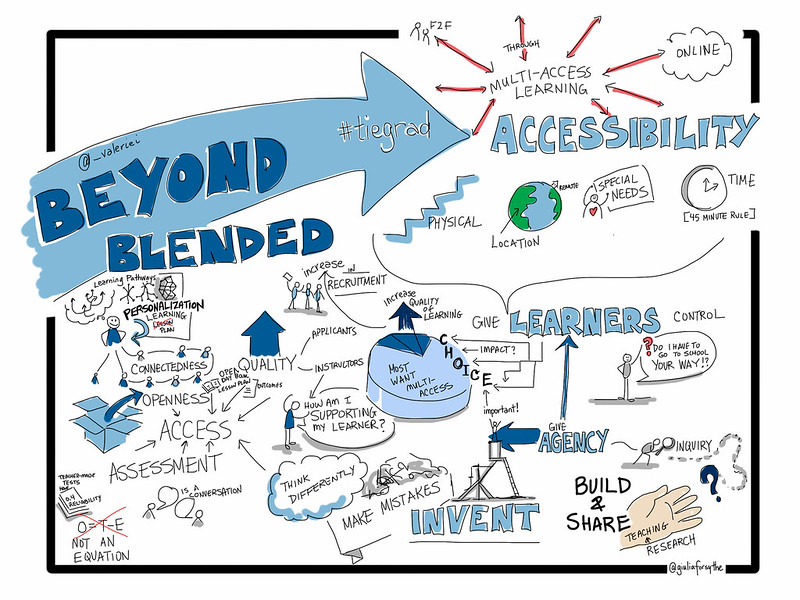
\includegraphics{assets/U5/U5LAImage.jpg}
\caption{Beyond Blended Visual notes by giuliaforsythe on Twitter}
\end{figure}

\hypertarget{unit-5-assessment}{%
\section*{Unit 5 Assessment}\label{unit-5-assessment}}
\addcontentsline{toc}{section}{Unit 5 Assessment}

\begin{feedback}
\hypertarget{things-to-do-this-week-1}{%
\subsubsection*{Things To Do This Week}\label{things-to-do-this-week-1}}
\addcontentsline{toc}{subsubsection}{Things To Do This Week}

✔️ Meet in Zoom {Wednesday, October 25 - 10:30 AM PDT} \href{https://www.timeanddate.com/worldclock/fixedtime.html?msg=LDRS663+Meeting\&iso=20231025T1030\&p1=1109\&ah=1}{Check your local time here}\\
✔️ \textbf{Read and Reflect} on the commentary in Unit 5.\\
✔️ \textbf{Publish} your \href{https://ma-lead.github.io/ldrs663/assessments.html\#showcase-post}{Showcase Post} using the category \texttt{ldrs663} and \texttt{showcase}.\\
✔️ Complete the \href{https://ma-lead.github.io/ldrs663/assessments.html\#facilitation-resource-project}{Facilitation Resource Project}.
✔️ Please complete these items by {Wednesday, November 8 - by sundown}, or let me know if you will need a bit more time.
\end{feedback}

\hypertarget{concluding-the-course}{%
\chapter{Concluding the Course}\label{concluding-the-course}}

Congratulations! We have taken a bit of a whirlwind tour through the main ideas of \emph{facilitating learning experiences} and \emph{coaching learners through challenges}. These two competencies form the backbone of the model of teaching and learning in the TWU GLOBAL FAR Centres and similar programs, and they are also highly transferable skills for anyone who is in a role that involves the acquisition of new cognitive skills.

These two related competencies are not `new' educational ideas, but are based in a long history of educational research showing the power of social constructivist pedagogies to transform thinking within a critical community of inquiry.

\hypertarget{blog-feeds}{%
\chapter*{Blog Feeds}\label{blog-feeds}}
\addcontentsline{toc}{chapter}{Blog Feeds}

\hypertarget{current-cohort}{%
\section*{Current Cohort}\label{current-cohort}}
\addcontentsline{toc}{section}{Current Cohort}

\hypertarget{past-cohorts}{%
\section*{Past Cohorts}\label{past-cohorts}}
\addcontentsline{toc}{section}{Past Cohorts}

Here is a list of posts from previous cohorts of this course. Keep in mind that we have changed the order of units several times over the years, so the post numbers and unit numbers will not likely align with the current cohort.

The purpose of providing these links is to allow you to see and evaluate the level of writing and reflection required during this course. You are welcome and encouraged to cite these posts by including the URL of the post on its own line in one of your posts.

\hypertarget{wordpress}{%
\chapter*{WordPress}\label{wordpress}}
\addcontentsline{toc}{chapter}{WordPress}

You are invited to document your learning in WordPress. This means that your work would be posted online on a public site. Keep in mind, though, that you are NOT required to post your work publicly. The steps below can help you decide how comfortable you are with sharing publicly.

Please review all 5 steps below to decide on your approach.

\hypertarget{decide-if-you-are-comfortable-posting-your-work-online.}{%
\subsection*{Decide if you are comfortable posting your work online.}\label{decide-if-you-are-comfortable-posting-your-work-online.}}
\addcontentsline{toc}{subsection}{Decide if you are comfortable posting your work online.}

If not, you can document your learning offline (with technology) by changing the privacy settings on your blog or using other offline tools. We would ask learners to consider using an online blogging tool with no identification/using a pseudonym, so as to develop network literacy, which is important in supporting learners, who are growing up in networked environments, but the preferences of learners will be respected and supported.

If you are comfortable being online, then proceed to step 2.

\hypertarget{would-you-like-to-use-your-real-name-or-use-a-pseudonym}{%
\subsection*{Would you like to use your real name or use a pseudonym?}\label{would-you-like-to-use-your-real-name-or-use-a-pseudonym}}
\addcontentsline{toc}{subsection}{Would you like to use your real name or use a pseudonym?}

You can claim your name online and own your presence by using your full name. With increasing catfishing and identity theft online, it can be helpful to have a presence that may compete with any fake profiles of you that are out there or to have a more dominant presence so posts or pictures of you by others may get drowned out. That said, you may wish to create an identity without your personal information (e.g., West coast teacher). The choice is yours.

With that decision made, proceed to step 3.

\hypertarget{decide-if-you-would-like-your-blog-to-be-hosted-outside-of-canada-or-inside-of-canada.}{%
\subsection*{Decide if you would like your blog to be hosted outside of Canada or inside of Canada.}\label{decide-if-you-would-like-your-blog-to-be-hosted-outside-of-canada-or-inside-of-canada.}}
\addcontentsline{toc}{subsection}{Decide if you would like your blog to be hosted outside of Canada or inside of Canada.}

We strongly recommend that you create a blog at \href{https://create.twu.ca}{create.twu.ca} which is built specifically for students and faculty at TWU, is hosted within Canada, and is completely free for you to use. You will not lose access to your site at create.twu.ca after you finish at TWU, but you are free to export it and publish it on your own space and on your own domain (e.g., \url{http://yourname.ca} or \url{http://westcoastteacher.ca}) with a web hosting company for a reasonable annual fee. Some of these companies host outside of Canada (e.g., Reclaim Hosting), while others host within Canada (e.g., Canadian Web Hosting).

With that decision made, proceed to step 4.

\hypertarget{you-also-have-to-decide-if-you-want-to-make-your-blog-public-or-private.}{%
\subsection*{You also have to decide if you want to make your blog public or private.}\label{you-also-have-to-decide-if-you-want-to-make-your-blog-public-or-private.}}
\addcontentsline{toc}{subsection}{You also have to decide if you want to make your blog public or private.}

You can set an entire blog to be private or simply selected posts can be set to private. You can set a password or invite people to gain access. We have provided instructions for adjusting your privacy settings on the tutorial page for opened.ca.

And last, but not least\ldots{}

\hypertarget{finally-you-have-to-think-about-where-you-and-your-content-will-end-up.}{%
\subsection*{Finally, you have to think about where you and your content will end up.}\label{finally-you-have-to-think-about-where-you-and-your-content-will-end-up.}}
\addcontentsline{toc}{subsection}{Finally, you have to think about where you and your content will end up.}

The wonderful thing about WordPress is that you can import that exported file into another WordPress instance (it sounds hard, but it isn't and we'll show you) or if you want to later set up your own domain and with your own WordPress installation. You may also import it into WordPress.com, but be aware that if you made posts with personal information knowing your site was hosted in Canada at the time and simply contained regular consent, without the specific consent for hosting outside of Canada, which requires you to name each tool, etc., you might not have consent to switch to WordPress.com. We often advise learners to post as if they will be on the cloud outside of Canada. To be honest, if you have a public blog, your friends and colleagues may be using U.S. cloud-hosted tools like Feedly to curate and read your blog posts or they may repost/quote your content on their U.S. blog. There are many educators who use U.S. software in their teaching and to support their learners. Just be sure to review how to get consent as per page four of the BC OIPC Cloud Computing Guidelines linked here.

\hypertarget{creating-a-blog}{%
\subsection*{Creating a Blog}\label{creating-a-blog}}
\addcontentsline{toc}{subsection}{Creating a Blog}

Once you have done all the reflections on these 5 steps, you can move forward with creating a blog. Please visit\href{https://create.twu.ca}{create.twu.ca}, click the green `Get Started' link and follow the instructions. Once you are done there, you can return here to continue with the next section to get your site set up.

\hypertarget{wordpress-setup}{%
\section{WordPress Setup}\label{wordpress-setup}}

\hypertarget{wordpress-resources}{%
\subsection*{WordPress Resources}\label{wordpress-resources}}
\addcontentsline{toc}{subsection}{WordPress Resources}

\begin{figure}
\centering
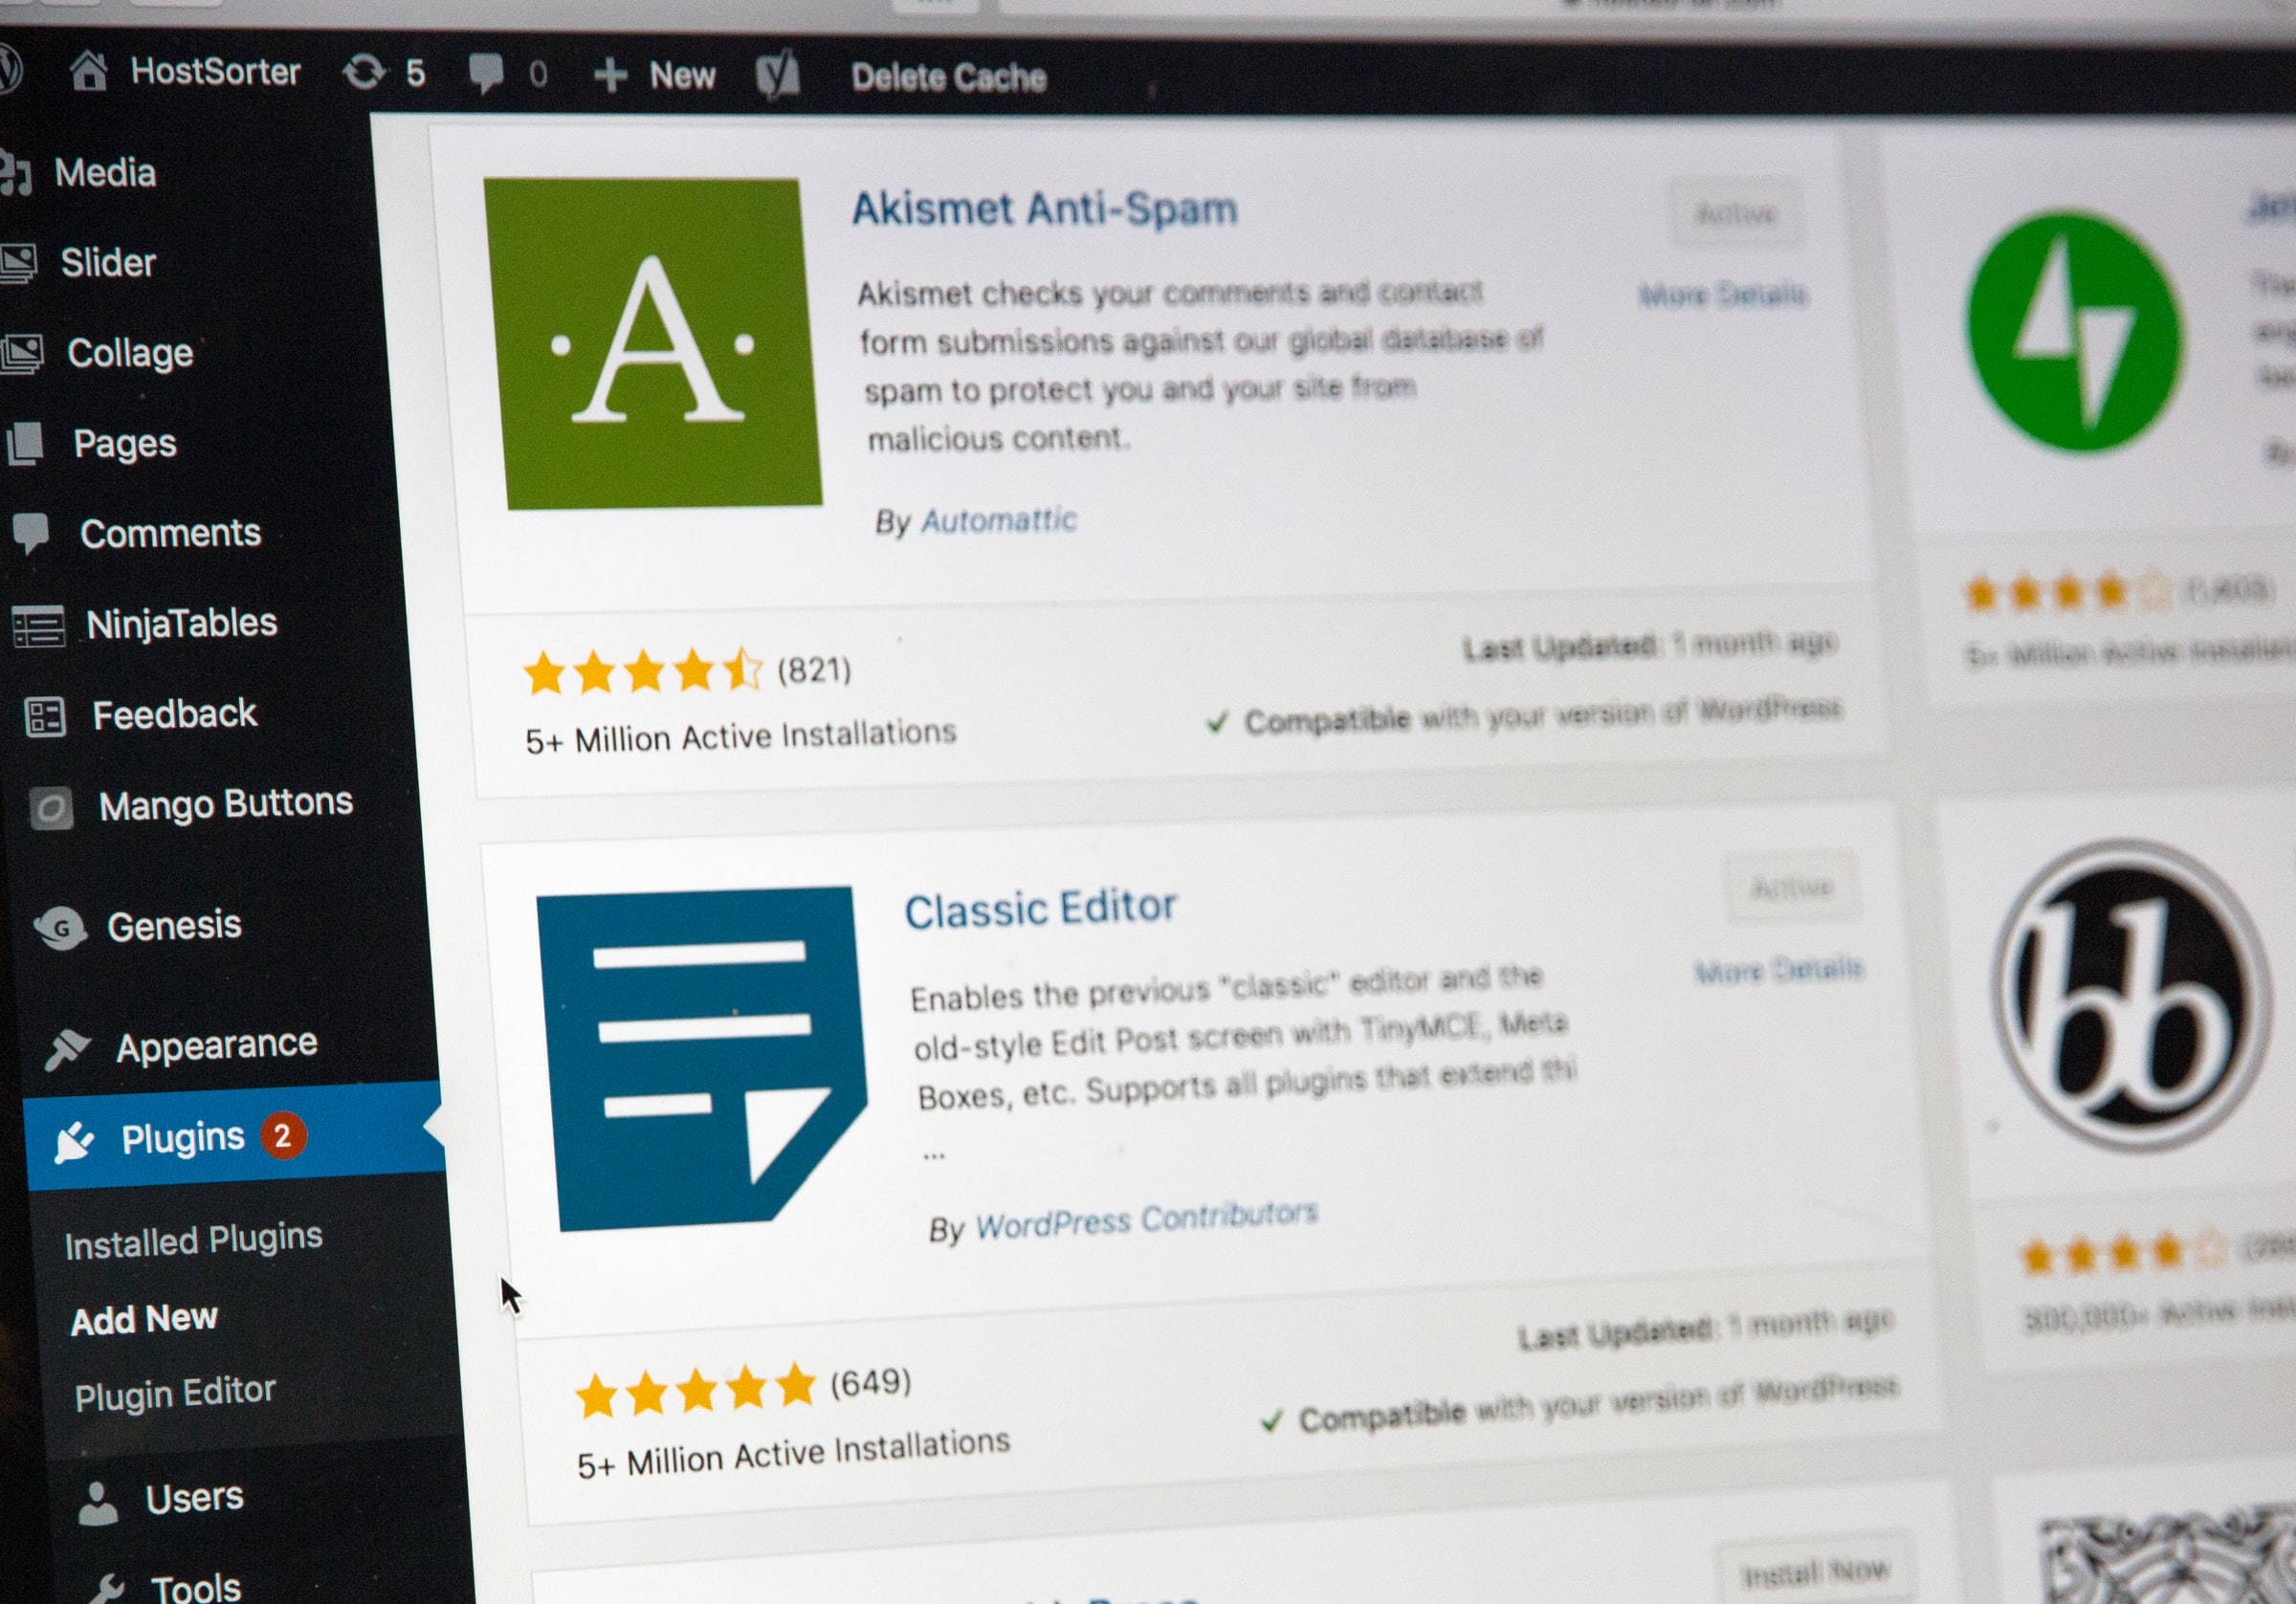
\includegraphics{assets/u1/stephen-phillips-hostreviews-co-uk-sSPzmL7fpWc-unsplash.jpg}
\caption{WordPress Dashboard (\href{https://unsplash.com/photos/sSPzmL7fpWc}{Image Credit})}
\end{figure}

We are here to help you create your site, so do not hesitate to ask for technical support. To get started on creating your site we suggest the following steps:

✔️ Log in if you have not already logged in; get familiar with the \href{http://sites.uci.edu/docs/start/dashboard/}{administration interface} and click \href{https://www.youtube.com/watch?v=-b569fs2t-Y}{here for more information on it}. The administration interface is also where the Dashboard in WordPress is located and \href{https://codex.wordpress.org/Dashboard_Screen}{you can get more info about it here.}\\
✔️ Remember: When you are in the site administration area of your site, you can get tips on what you are doing by clicking the ``Help'' menu on the top-right corner.\\
✔️ Review your settings, start by changing your Site Title under \texttt{Settings\textgreater{}General}. You need to hit the ``Save'' button to save your changes. \href{https://codex.wordpress.org/Settings_General_Screen}{More information about General Settings here.}\\
✔️ \href{http://www.wpbeginner.com/beginners-guide/how-to-add-a-new-post-in-wordpress-and-utilize-all-the-features/}{Add a new post}{]}. You can pick one of the existing categories by checking a box on the sidebar of the authoring interface. \href{http://www.wpbeginner.com/glossary/category/}{You can manage your categories here.} You will need to hit the blue ``Publish'' button on the right hand side before your post appears. \href{https://en.support.wordpress.com/pages/page-visibility/}{Information on managing the privacy settings on individual posts is here.}\\
✔️ Edit your about me page by introducing yourself and sharing a little about yourself.\\
✔️ You are welcome to change the images and upload your own. \href{https://www.youtube.com/watch?v=GtMOAaMFaPs}{Here is information about using images from Google.}

\hypertarget{wordpress-tutorials}{%
\section{WordPress Tutorials}\label{wordpress-tutorials}}

When you're ready to start customizing your blog and putting content in, check out some tutorials available to you:

✔️ \href{http://www.wpbeginner.com/start-here/}{Beginner's guide for WordPress by WPBeginner}\\
✔️ \href{https://learn.wordpress.com/}{Learn WordPress website by WordPress}\\
✔️ \href{http://digitaltattoo.ubc.ca/}{Digital Tattoo Project at UBC} -- learn digital literacy skills. Check out the menu sections and \href{http://digitaltattoo.ubc.ca/publish/}{consider looking at the publish section.}

If you are confused about anything it is always good to do an initial Google or YouTube search, or reach out to your learning pod or your instructor.

  \bibliography{book.bib}

\end{document}
